\section{บทที่ 8 การควบคุม การเขียนโปรแกรม และการบำรุงรักษาหุ่นยนต์อุตสาหกรรม}

\begin{tabularx}{\textwidth}{@{}L{0.24\textwidth}Y@{}}
\textbf{ชื่อบทภาษาอังกฤษ:} & Automation Systems and Industrial Robot Applications \\
\textbf{รายวิชา:} & หุ่นยนต์ในระบบงานอุตสาหกรรม (Industrial Robots) \\
\textbf{รหัสวิชา:} & 5574506 \\
\textbf{หน่วยกิต:} & 3(1-4-4) \\
\end{tabularx}


\subsection{1. แนวคิดสำคัญของบท}

หุ่นยนต์อุตสาหกรรมจะสร้างคุณค่าให้กระบวนการผลิตได้ต่อเมื่อผู้ใช้งานสามารถกำหนดตำแหน่งและทิศทางของเครื่องมือ วางแผนเส้นทาง เขียนลำดับการทำงาน เชื่อมต่อสัญญาณกับอุปกรณ์ภายนอก และตรวจสอบความปลอดภัยได้อย่างเป็นระบบ การเขียนโปรแกรมหุ่นยนต์จึงไม่ใช่เพียงการบันทึกจุดแล้วสั่งให้เคลื่อนที่ แต่เป็นการประสานความรู้ด้านระบบพิกัด จลนศาสตร์ การควบคุมการเคลื่อนที่ ลอจิก โปรแกรม PLC อุปกรณ์จับยึด และข้อกำหนดด้านความปลอดภัย

ในอีกด้านหนึ่ง หุ่นยนต์อุตสาหกรรมเป็นสินทรัพย์ที่มีอายุใช้งานยาวนาน โดยทั่วไปอาจถูกใช้งานต่อเนื่องเป็นเวลาหลายปีภายใต้สภาพโหลด รอบการทำงาน และสภาพแวดล้อมที่แตกต่างกัน การบำรุงรักษาเชิงป้องกัน (Preventive Maintenance: PM) การติดตามสภาพ (Condition Monitoring) การจัดเก็บประวัติ Alarm และการทวนสอบ Calibration จึงมีผลโดยตรงต่อความพร้อมใช้งาน ความแม่นยำ คุณภาพผลิตภัณฑ์ และความปลอดภัย

สาระสำคัญของบทประกอบด้วย 7 แกนหลัก ได้แก่

\begin{enumerate}
    \item การเลือกและใช้งานระบบพิกัดของหุ่นยนต์
    \item การสอนตำแหน่งด้วย Teach Pendant และการเขียนโปรแกรมแบบ Offline
    \item การเลือก Motion Command และการวางแผนเส้นทาง
    \item การสร้างโปรแกรม Motion, I/O และ Logic ที่ตรวจสอบได้
    \item การจัดทำแผน PM และบันทึกประวัติการบำรุงรักษา
    \item การวิเคราะห์ Alarm และแก้ไขปัญหาอย่างเป็นระบบ
    \item การควบคุมความเสี่ยงตามมาตรฐานความปลอดภัยของหุ่นยนต์และเครื่องจักร
\end{enumerate}

\par\noindent\rule{\textwidth}{0.4pt}\par

\subsection{2. ความรู้พื้นฐานก่อนเรียน}

ก่อนเรียนบทนี้ นักศึกษาควรมีความรู้หรือทักษะดังต่อไปนี้

\begin{itemize}
    \item โครงสร้างหุ่นยนต์อุตสาหกรรมแบบหลายแกน ข้อต่อ และแกนการเคลื่อนที่
    \item ความหมายของ Position, Orientation, Joint และ End Effector
    \item หลักการพื้นฐานของ Forward Kinematics และ Inverse Kinematics
    \item การทำงานของ Servo Motor, Encoder, Brake และ Robot Controller
    \item สัญญาณ Digital Input/Output และหลักการ Interlock
    \item หลักการใช้ Emergency Stop, Safety Gate และ Enabling Device
    \item พื้นฐานการอ่าน Wiring Diagram และการตรวจสอบ Connector
    \item การใช้หน่วย SI เช่น มิลลิเมตร องศา วินาที นิวตัน และกิโลกรัม
\end{itemize}

หากผู้เรียนยังไม่เคยใช้หุ่นยนต์จริง ควรเริ่มจากซอฟต์แวร์จำลองหรือโหมดฝึกอบรมของ Controller ก่อนเข้าสู่การ Jog และการทดสอบโปรแกรมบนหุ่นยนต์จริง

\par\noindent\rule{\textwidth}{0.4pt}\par

\subsection{3. คำสำคัญประจำบท}

\begin{table}[htbp]
    \centering
    \small
    \begin{tabularx}{\textwidth}{@{}L{0.22\textwidth}L{0.28\textwidth}Y@{}}
        \hline
        \textbf{คำศัพท์ภาษาไทย} & \textbf{คำศัพท์ภาษาอังกฤษ} & \textbf{ความหมายโดยย่อ} \\
        \hline
        ระบบพิกัดข้อต่อ & Joint Coordinate System & ระบบพิกัดที่อธิบายตำแหน่งด้วยค่ามุมหรือระยะของแต่ละ Joint \\
        ระบบพิกัดฐาน/โลก & Base/World Coordinate System & ระบบพิกัดคาร์ทีเซียนที่อ้างอิงกับฐานหรือกรอบอ้างอิงหลักของหุ่นยนต์ \\
        ระบบพิกัดเครื่องมือ & Tool Coordinate System & ระบบพิกัดที่ผูกกับเครื่องมือ โดยจุดกำเนิดมักอยู่ที่ TCP \\
        ระบบพิกัดผู้ใช้ & User/Work Object Coordinate System & ระบบพิกัดที่ผู้ใช้กำหนดให้สัมพันธ์กับ Fixture หรือชิ้นงาน \\
        จุดศูนย์กลางเครื่องมือ & Tool Center Point: TCP & จุดอ้างอิงของ End Effector ที่ใช้คำนวณตำแหน่งและเส้นทาง \\
        การสอนตำแหน่ง & Teaching & การนำหุ่นยนต์ไปยัง Pose ที่ต้องการและบันทึกเป็นจุดในโปรแกรม \\
        แผงสอน & Teach Pendant & อุปกรณ์ควบคุมสำหรับ Jog ตั้งค่า สอนตำแหน่ง และทดสอบโปรแกรม \\
        การนำแขนด้วยมือ & Lead-through/Hand Guiding & การนำหุ่นยนต์ไปตามท่าหรือเส้นทางด้วยแรงจากผู้ใช้ในโหมดที่รองรับ \\
        การเขียนโปรแกรมนอกสายการผลิต & Offline Programming: OLP & การสร้างและจำลองโปรแกรมบนคอมพิวเตอร์โดยไม่ครอบครองหุ่นยนต์จริง \\
        การเคลื่อนที่แบบจุดต่อจุด & Point-to-Point: PTP & การเคลื่อนที่ที่วางแผนใน Joint Space โดยไม่รับประกันเส้นทาง TCP \\
        การเคลื่อนที่เชิงเส้น & Linear Motion: LIN & การเคลื่อนที่ที่ควบคุมให้ TCP เคลื่อนเป็นเส้นตรงใน Cartesian Space \\
        การเคลื่อนที่เป็นวงโค้ง & Circular Motion: CIRC & การเคลื่อนที่ที่ให้ TCP ผ่านจุดกลางและจุดปลายเป็นส่วนโค้ง \\
        การกลมมุม & Blending/Zone/CNT & การไม่หยุดสนิทที่จุดผ่านเพื่อให้เส้นทางต่อเนื่องและลด Cycle Time \\
        ตำแหน่งละเอียด & Fine Point & จุดที่กำหนดให้หุ่นยนต์เข้าใกล้เป้าหมายตามเกณฑ์ก่อนทำคำสั่งถัดไป \\
        สัญญาณประสานงาน & Handshake Signal & ชุดสัญญาณ Request, Ready, Busy, Complete และ Fault ระหว่างอุปกรณ์ \\
        การทำ Mastering & Mastering & การกำหนดความสัมพันธ์ระหว่างค่าตำแหน่ง Encoder กับตำแหน่งอ้างอิงของแกน \\
        การสอบเทียบ & Calibration & การตรวจสอบและปรับความสัมพันธ์ระหว่างค่าที่ระบบรายงานกับตำแหน่งจริง \\
        การบำรุงรักษาเชิงป้องกัน & Preventive Maintenance: PM & การบำรุงรักษาตามเวลา ชั่วโมงทำงาน หรือรอบการทำงานก่อนเกิดความขัดข้อง \\
        การบำรุงรักษาตามสภาพ & Condition-based Maintenance & การบำรุงรักษาเมื่อข้อมูลสภาพบ่งชี้แนวโน้มเสื่อมสภาพ \\
        การแก้ไขปัญหา & Troubleshooting & กระบวนการระบุสาเหตุ ทดสอบสมมติฐาน แก้ไข และยืนยันผลอย่างเป็นระบบ \\
        การล็อกและติดป้าย & Lockout/Tagout: LOTO & การแยกแหล่งพลังงาน ล็อกอุปกรณ์ และติดป้ายก่อนงานซ่อมบำรุง \\
        ระยะป้องกัน & Safeguard Separation Distance & ระยะขั้นต่ำระหว่างอุปกรณ์ตรวจจับ/รั้วกับอันตรายตามเวลาหยุดและการเข้าถึง \\
        เขตเตือน & Warning Zone & เขตที่ระบบแจ้งเตือนหรือจำกัดพฤติกรรมก่อนถึงเขตอันตราย \\
        เขตป้องกัน & Protective Zone & เขตที่การบุกรุกต้องทำให้เกิด Protective Stop หรือมาตรการที่กำหนด \\
        ความพร้อมใช้งาน & Availability & สัดส่วนเวลาที่ระบบพร้อมทำงานเทียบกับเวลาที่วางแผนให้ทำงาน \\
        \hline
    \end{tabularx}
\end{table}

\par\noindent\rule{\textwidth}{0.4pt}\par

\subsection{4. ผลลัพธ์การเรียนรู้ประจำบท}

\begin{quote}
เมื่อเรียนจบบทนี้ นักศึกษาสามารถ...
\end{quote}

\begin{enumerate}
    \item \textbf{อธิบายและเลือกใช้} Joint, World/Base, Tool และ User/Work Object Coordinate System ให้เหมาะกับภารกิจได้
    \item \textbf{สอนตำแหน่งและทวนสอบ} TCP, User Frame และจุดทำงานด้วย Teach Pendant ในโหมดที่ปลอดภัยได้
    \item \textbf{เขียนและตรวจสอบ} โปรแกรมหุ่นยนต์เบื้องต้นที่ใช้ Motion, I/O, Logic, Subroutine และ Interlock ได้
    \item \textbf{วิเคราะห์และเลือก} PTP, Linear, Circular และ Blending ให้เหมาะกับความแม่นยำ คุณภาพเส้นทาง และ Cycle Time ได้
    \item \textbf{จัดทำและประเมิน} แผน Preventive Maintenance พร้อมแบบบันทึกและเกณฑ์ติดตามสภาพได้
    \item \textbf{วิเคราะห์ Alarm และดำเนินการ Troubleshooting} โดยไม่สร้างความเสี่ยงเพิ่มเติมแก่บุคลากรหรืออุปกรณ์ได้
    \item \textbf{ปฏิบัติตาม} หลัก Safeguarding, Reduced-speed Teaching และ LOTO ในการใช้งานและบำรุงรักษาหุ่นยนต์ได้
\end{enumerate}

\subsubsection{ตาราง 8.1 ความสอดคล้องระหว่างผลลัพธ์ เนื้อหา กิจกรรม และการประเมิน}

\begin{table}[htbp]
    \centering
    \small
    \begin{tabularx}{\textwidth}{@{}L{0.08\textwidth}L{0.24\textwidth}L{0.24\textwidth}L{0.18\textwidth}Y@{}}
        \hline
        \textbf{CLO} & \textbf{เนื้อหาที่เกี่ยวข้อง} & \textbf{กิจกรรมการเรียนรู้} & \textbf{วิธีประเมิน} & \textbf{หลักฐานการเรียนรู้} \\
        \hline
        CLO1 & ระบบพิกัดและการแปลงกรอบอ้างอิง & วิเคราะห์ภาพ Coordinate และเลือกกรอบอ้างอิง & แบบทดสอบสั้นและคำถามปากเปล่า & ตารางเลือก Coordinate พร้อมเหตุผล \\
        CLO2 & TCP Calibration, User Frame, Teaching & ใบงาน 8-1 สอนตำแหน่ง 5 จุด & สังเกตการปฏิบัติและตรวจจุด & Point List, ค่า Frame และ Checklist \\
        CLO3 & Motion, I/O, Logic, Handshake & เขียน Pick-and-Place และ Dry Run & ตรวจโปรแกรมและทดสอบใน T1 & ไฟล์โปรแกรมและผลทดสอบ \\
        CLO4 & PTP, LIN, CIRC, FINE, CNT/Zone & เปรียบเทียบเส้นทางและ Cycle Time & วิเคราะห์กรณีศึกษา & ตารางเลือก Motion และค่าปรับ \\
        CLO5 & PM Schedule, Record, Calibration & ใบงาน 8-2 ตรวจสภาพและวางแผน PM & ตรวจแบบฟอร์มและ Rubric & Daily Checklist และ PM Record \\
        CLO6 & Alarm, Root Cause, Verification & ใบงาน 8-3 จำลอง Alarm อย่างปลอดภัย & ประเมินขั้นตอนและรายงาน & Troubleshooting Report \\
        CLO7 & ISO 10218, ISO 13855, LOTO & Pre-job Briefing และ Safety Walkdown & Practical Safety Check & แบบประเมินความปลอดภัยและ LOTO Checklist \\
        \hline
    \end{tabularx}
\end{table}

\par\noindent\rule{\textwidth}{0.4pt}\par

\subsection{5. แผนผังเนื้อหาของบท}

\begin{verbatim}
ระบบพิกัดและ TCP
        |
การ Jog และการสอนตำแหน่ง
        |
Motion Command และ Path Planning
        |
โครงสร้างโปรแกรม Motion–I/O–Logic
        |
Simulation / Dry Run / Validation
        |
การใช้งานจริงและการเก็บข้อมูล
        |
Preventive Maintenance และ Calibration
        |
Troubleshooting และ Safe Recovery
        |
Safeguarding, Risk Assessment และ LOTO
\end{verbatim}

ลำดับดังกล่าวสะท้อนวงจรชีวิตของโปรแกรมหุ่นยนต์ ตั้งแต่การกำหนดกรอบอ้างอิง การสร้างเส้นทาง การทดสอบ การใช้งาน การบำรุงรักษา ไปจนถึงการกู้คืนระบบหลังเกิดความผิดปกติ

\par\noindent\rule{\textwidth}{0.4pt}\par

\subsection{6. บทนำ}

ในสายการผลิตสมัยใหม่ หุ่นยนต์อุตสาหกรรมมักทำงานร่วมกับ Conveyor, Vision System, PLC, Safety PLC, Gripper, Welding Power Source, Positioner และเครื่องจักรอื่น โปรแกรมหุ่นยนต์จึงต้องตอบคำถามสำคัญอย่างน้อย 5 ข้อ ได้แก่

\begin{enumerate}
    \item \textbf{หุ่นยนต์ต้องไปที่ใด} — กำหนดด้วย Position, Orientation และ Coordinate Frame
    \item \textbf{ต้องไปอย่างไร} — เลือก PTP, Linear, Circular, Speed, Acceleration และ Blending
    \item \textbf{ไปเมื่อใด} — กำหนดด้วย I/O, Interlock, Wait, Timer และ State ของกระบวนการ
    \item \textbf{เมื่อผิดปกติจะทำอย่างไร} — กำหนด Alarm Handling, Recovery Position และเงื่อนไข Restart
    \item \textbf{จะรักษาความปลอดภัยและความพร้อมใช้งานอย่างไร} — ใช้ Safeguarding, PM, Calibration, Backup และ LOTO
\end{enumerate}

ตัวอย่างเช่น งานหยิบชิ้นงานจาก Conveyor ไม่สามารถใช้เพียงคำสั่งเคลื่อนที่ไปยังจุด Pick ได้ โปรแกรมต้องตรวจว่ามีชิ้นงานจริง Gripper พร้อมทำงาน พื้นที่ปลายทางว่าง และระบบ Safety อยู่ในสถานะอนุญาต เมื่อตรวจครบแล้วจึงเคลื่อนที่ไปยังจุด Approach ลดความเร็วเข้าสู่จุด Pick สั่งจับ รอสัญญาณ Gripper Confirm ถอยออกตามแนวปลอดภัย และส่งสถานะ Complete ให้ PLC หากสัญญาณยืนยันไม่มาในเวลาที่กำหนด โปรแกรมต้องหยุดอย่างควบคุม แจ้ง Alarm และไม่เคลื่อนต่อโดยคาดเดาว่าจับชิ้นงานสำเร็จ

แนวคิดสำคัญจึงอยู่ที่การทำให้ \textbf{ตำแหน่ง เส้นทาง ลอจิก การบำรุงรักษา และความปลอดภัย} เป็นระบบเดียวกัน ไม่ใช่ส่วนแยกจากกัน

\par\noindent\rule{\textwidth}{0.4pt}\par

\subsection{7. เนื้อหาหลัก}

\subsection{7.1 ระบบพิกัดในหุ่นยนต์อุตสาหกรรม}

\subsubsection{7.1.1 เหตุผลที่ต้องมีหลายระบบพิกัด}

หุ่นยนต์ 6 แกนสามารถอธิบายท่าทางเดียวกันได้หลายรูปแบบ เช่น อธิบายด้วยมุม Joint ทั้งหก หรืออธิบายด้วยพิกัด $X,Y,Z$ และมุม Orientation ของ TCP เมื่อผู้ปฏิบัติงาน Jog หุ่นยนต์ สิ่งที่ต้องการควบคุมอาจเป็น “หมุนเฉพาะแกน 2” “เลื่อนไปทางแกน $Z$ ของฐาน” “เดินหัวเชื่อมไปข้างหน้าตามแกนของ Torch” หรือ “เลื่อนตามแนวขอบ Fixture” การมี Coordinate System หลายแบบทำให้คำสั่งสอดคล้องกับเจตนาของงาน

\subsubsection{7.1.2 Joint Coordinate System}

Joint Coordinate System กำหนดสถานะของหุ่นยนต์ด้วยเวกเตอร์ค่าข้อต่อ

\[
\mathbf{q} = [q_1,q_2,\ldots,q_n]^T
\]

สำหรับหุ่นยนต์หมุน 6 แกน มักเขียนเป็น

\[
\mathbf{q} = [\theta_1,\theta_2,\theta_3,\theta_4,\theta_5,\theta_6]^T
\]

โดย $\theta_i$ คือมุมของ Joint ที่ $i$ หน่วยองศาหรือเรเดียนตามระบบ Controller

\textbf{ลักษณะสำคัญ}

\begin{itemize}
    \item ปุ่ม Jog แต่ละปุ่มสั่งแกนใดแกนหนึ่งหรือหลายแกนตามโหมดของ Controller
    \item เหมาะสำหรับหลบสิ่งกีดขวาง แก้ท่าทางใกล้ Singularity และกลับสู่ท่าอ้างอิง
    \item เส้นทาง TCP ระหว่างจุดเริ่มและจุดปลายอาจเป็นเส้นโค้งที่คาดเดาได้ยาก
    \item การเคลื่อน Joint หนึ่งแกนอาจทำให้ TCP เคลื่อนที่เป็นระยะมาก โดยเฉพาะแกนใกล้ฐาน
\end{itemize}

\textbf{ข้อควรระวัง:} การ Jog ใน Joint Coordinate ต้องมองทั้งแขน ไม่ใช่มองเฉพาะ TCP เพราะส่วน Elbow, Wrist หรือสาย Dress Pack อาจเข้าใกล้โครงสร้างอื่นก่อนที่ TCP จะถึงสิ่งกีดขวาง

\subsubsection{7.1.3 World หรือ Base Coordinate System}

World/Base Coordinate System เป็นกรอบพิกัดคาร์ทีเซียนที่ผูกกับฐานหุ่นยนต์หรือกรอบหลักของเซลล์ ตำแหน่ง TCP เขียนได้เป็น

\[
\mathbf{x} = [x,y,z,\alpha,\beta,\gamma]^T
\]

โดย $x,y,z$ เป็นตำแหน่ง หน่วยมิลลิเมตรหรือเมตร และ $\alpha,\beta,\gamma$ เป็นตัวแทน Orientation ซึ่งรูปแบบจริงอาจเป็น Euler Angle, Roll–Pitch–Yaw, Quaternion หรือ Axis–Angle ตามผู้ผลิต

\textbf{เหมาะสำหรับ}

\begin{itemize}
    \item เคลื่อนที่ขึ้น–ลงหรือซ้าย–ขวาตามโครงสร้างเซลล์
    \item ตรวจสอบ Working Envelope และตำแหน่งสัมพันธ์กับรั้วหรือเครื่องจักร
    \item การประสานหลายอุปกรณ์เมื่อทุกอุปกรณ์อ้างอิงกรอบกลางเดียวกัน
\end{itemize}

\textbf{ข้อจำกัด:} หาก Fixture ถูกย้าย การแก้จุดทุกจุดใน World Frame อาจใช้เวลามาก จึงควรสร้าง User Frame ให้ผูกกับ Fixture

\subsubsection{7.1.4 Tool Coordinate System และ Tool Center Point}

Tool Coordinate System ผูกกับ End Effector จุดกำเนิดมักกำหนดที่ \textbf{Tool Center Point (TCP)} เช่น ปลายลวดเชื่อม จุดกึ่งกลางหัวพ่น หรือจุดกึ่งกลางระหว่างนิ้ว Gripper

การ Jog ใน Tool Coordinate มีประโยชน์อย่างมากเมื่อผู้ปฏิบัติงานต้องการ

\begin{itemize}
    \item เดินหัวเชื่อมตามแกนของ Torch
    \item เลื่อนหัวเจาะเข้า–ออกตามแนวแกนดอกสว่าน
    \item ถอย Gripper ออกจากชิ้นงานตามแนวปลอดภัย
    \item ปรับ Standoff Distance ของหัวพ่นหรือกล้อง
\end{itemize}

หาก TCP กำหนดผิด การเคลื่อนที่ Linear อาจทำให้จุดที่ต้องการใช้งานจริงไม่เดินตามเส้นตรง แม้ Controller จะคำนวณเส้นทางของ TCP ที่กำหนดไว้ได้ถูกต้องก็ตาม

\textbf{แนวทาง TCP Calibration ที่พบบ่อย}

\begin{enumerate}
    \item \textbf{Three-point/Four-point method:} นำปลายเครื่องมือแตะจุดอ้างอิงเดียวกันด้วย Orientation หลายค่าเพื่อหาตำแหน่ง TCP
    \item \textbf{Six-point method:} ใช้หลาย Pose เพื่อคำนวณทั้งตำแหน่งและ Orientation ของ Tool Frame
    \item \textbf{Direct entry:} ป้อนค่าจาก CAD หรือ Drawing เมื่อมิติและการติดตั้งมีความน่าเชื่อถือ
    \item \textbf{External measurement:} ใช้ Jig, Probe, Laser Tracker หรือ Metrology System ในงานที่ต้องการความแม่นยำสูง
\end{enumerate}

\subsubsection{7.1.5 User Coordinate System หรือ Work Object}

User Frame หรือ Work Object เป็นกรอบพิกัดที่ผูกกับ Fixture, Pallet, Table หรือชิ้นงาน โปรแกรมที่สร้างจุดสัมพันธ์กับกรอบนี้สามารถย้ายตาม Fixture ได้โดยแก้ค่ากรอบเพียงชุดเดียว แทนการแก้ทุกจุด

ตัวอย่างเช่น โปรแกรมวางชิ้นงานลงถาด 2 × 5 ช่อง สามารถกำหนดจุดเริ่มต้น $P_{00}$ และระยะ Pitch ตามแกนของ User Frame ดังนี้

\[
\mathbf{p}_{ij}=\mathbf{p}_{00}+i\Delta x\hat{\mathbf{x}}_U+j\Delta y\hat{\mathbf{y}}_U
\]

เมื่อ

\begin{itemize}
    \item $i$ คือดัชนีคอลัมน์
    \item $j$ คือดัชนีแถว
    \item $\Delta x$ คือระยะห่างคอลัมน์
    \item $\Delta y$ คือระยะห่างแถว
    \item $\hat{\mathbf{x}}_U,\hat{\mathbf{y}}_U$ คือเวกเตอร์หน่วยของ User Frame
\end{itemize}

หากถาดถูกเลื่อนหรือหมุน สามารถสอน User Frame ใหม่โดยไม่ต้องแก้สูตร Offset ของทุกช่อง

\subsubsection{7.1.6 การแปลงกรอบอ้างอิง}

ความสัมพันธ์ระหว่างกรอบพิกัดนิยมเขียนด้วย Homogeneous Transformation Matrix ขนาด $4\times4$

\[
{}^{A}\mathbf{T}_{B}=
\begin{bmatrix}
{}^{A}\mathbf{R}_{B} & {}^{A}\mathbf{p}_{B}\\
\mathbf{0}^T & 1
\end{bmatrix}
\]

โดย

\begin{itemize}
    \item ${}^{A}\mathbf{R}_{B}$ คือเมทริกซ์การหมุนของกรอบ $B$ เมื่อมองจากกรอบ $A$
    \item ${}^{A}\mathbf{p}_{B}$ คือเวกเตอร์ตำแหน่งจุดกำเนิดของกรอบ $B$ เมื่อมองจากกรอบ $A$
\end{itemize}

หากทราบตำแหน่ง User Frame เทียบกับ Base และทราบ TCP เทียบกับ User Frame จะหาตำแหน่ง TCP เทียบกับ Base ได้จาก

\[
{}^{B}\mathbf{T}_{TCP} = {}^{B}\mathbf{T}_{U}\,{}^{U}\mathbf{T}_{TCP}
\]

สมการนี้อธิบายเหตุผลที่การแก้ ${}^{B}\mathbf{T}_{U}$ เพียงค่าเดียวสามารถย้ายจุดทั้งหมดที่สอนใน User Frame ไปพร้อมกัน

\textbf{สมมติฐานและข้อจำกัด}

\begin{itemize}
    \item กรอบทุกกรอบต้องกำหนดตาม Convention เดียวกับ Controller
    \item ลำดับการหมุนมีผลต่อค่า Orientation
    \item ความคลาดเคลื่อนของ Tool Frame และ User Frame จะสะสมเข้าสู่ตำแหน่ง TCP
    \item การแปลงกรอบถูกต้องทางคณิตศาสตร์ไม่ได้รับประกันว่าหุ่นยนต์จะเข้าถึง Pose ได้หรือไม่ชนสิ่งกีดขวาง
\end{itemize}

\subsubsection{ตัวอย่างที่ 8.1 การคำนวณ Offset ของถาดใน User Frame}

\textbf{ตัวอย่างเพิ่มเติมเพื่อการเรียนรู้}

ถาดมี 2 แถว 5 คอลัมน์ จุดแรกอยู่ที่ $(x,y,z)=(100,50,20)$ mm ใน User Frame ระยะห่างคอลัมน์ 40 mm และระยะห่างแถว 60 mm จงหาตำแหน่งช่องแถวที่ 2 คอลัมน์ที่ 4 โดยกำหนดดัชนีเริ่มที่ศูนย์

\textbf{วิเคราะห์โจทย์}

\begin{itemize}
    \item แถวที่ 2 ให้ $j=1$
    \item คอลัมน์ที่ 4 ให้ $i=3$
    \item $\Delta x=40$ mm และ $\Delta y=60$ mm
\end{itemize}

\[
\mathbf{p}_{31}=
\begin{bmatrix}100\\50\\20\end{bmatrix}
+3\begin{bmatrix}40\\0\\0\end{bmatrix}
+1\begin{bmatrix}0\\60\\0\end{bmatrix}
\]

ดังนั้น

\[
\mathbf{p}_{31}=
\begin{bmatrix}220\\110\\20\end{bmatrix}\text{ mm}
\]

\textbf{ตรวจสอบความสมเหตุสมผล:} คอลัมน์เพิ่ม 3 ช่วงจึงเพิ่ม $120$ mm และแถวเพิ่ม 1 ช่วงจึงเพิ่ม $60$ mm ค่า $z$ คงเดิม

\subsubsection{ตาราง 8.2 แนวทางเลือกระบบพิกัด}

\begin{table}[htbp]
    \centering
    \begin{tabular}{l l l}
        \hline
        \textbf{งานที่ต้องทำ} & \textbf{Coordinate ที่เหมาะสม} & \textbf{เหตุผล} \\
        \hline
        หลบ Elbow ออกจากโครงสร้าง & Joint & ควบคุมแกนเฉพาะและเห็นผลต่อท่าทางแขน \\
        ยก TCP ขึ้นในแนวดิ่งของเซลล์ & World/Base & เคลื่อนตามแกนคงที่ของพื้นที่ทำงาน \\
        เดินหัวเชื่อมเข้า–ออกตามแนว Torch & Tool & แกนเคลื่อนที่ติดกับ Orientation ของเครื่องมือ \\
        สอนจุดบน Fixture ที่อาจถูกย้าย & User/Work Object & แก้ Frame แทนการแก้ทุก Point \\
        กลับท่า Home ที่กำหนดเป็นค่าข้อต่อ & Joint & ท่าหุ่นยนต์กำหนดชัดเจนด้วยค่า Joint \\
        วาง Pattern บนถาด & User + Offset & สร้างจุดจาก Pitch ของถาดได้ง่าย \\
        \hline
    \end{tabular}
\end{table}

% [รูปที่ 8.1: ระบบพิกัด World, Tool และ User บนหุ่นยนต์ 6 แกน]
% ประเภทภาพ: Technical Illustration
% ตำแหน่งที่แนะนำ: หลังหัวข้อ 7.1
% วัตถุประสงค์การเรียนรู้: แสดงความแตกต่างของกรอบอ้างอิงและจุด TCP
% คำอธิบายภาพ: หุ่นยนต์ 6 แกนติด Gripper มีกรอบ World ที่ฐาน กรอบ Tool ที่ TCP และกรอบ User บน Fixture พร้อมแกน X–Y–Z ตาม Right-hand Rule
% องค์ประกอบที่ต้องมี: Robot Base, Joint 1–6, End Effector, TCP, Fixture, Workpiece, World Frame, Tool Frame, User Frame และลูกศรแกน
% ข้อความหรือป้ายกำกับ: World/Base, Tool/TCP, User/Work Object, Joint 1–6
% ภาษาของป้ายกำกับ: ไทยและอังกฤษ
% สัดส่วนภาพ: 16:9
% Image Generation Prompt: Engineering textbook technical illustration of a six-axis industrial robot with three clearly distinguished coordinate frames: World/Base frame at the robot base, Tool frame at the gripper TCP, and User/Work Object frame attached to a fixture. Show X, Y, Z axes using the right-hand convention, label joints 1 to 6, end effector, TCP, fixture and workpiece. Clean white background, precise vector lines, bilingual Thai-English labels, no decorative elements, 16:9.
% Alt Text: หุ่นยนต์ 6 แกนที่แสดงกรอบ World ที่ฐาน กรอบ Tool ที่ TCP และกรอบ User บน Fixture

\begin{figure}[htbp]
    \centering
    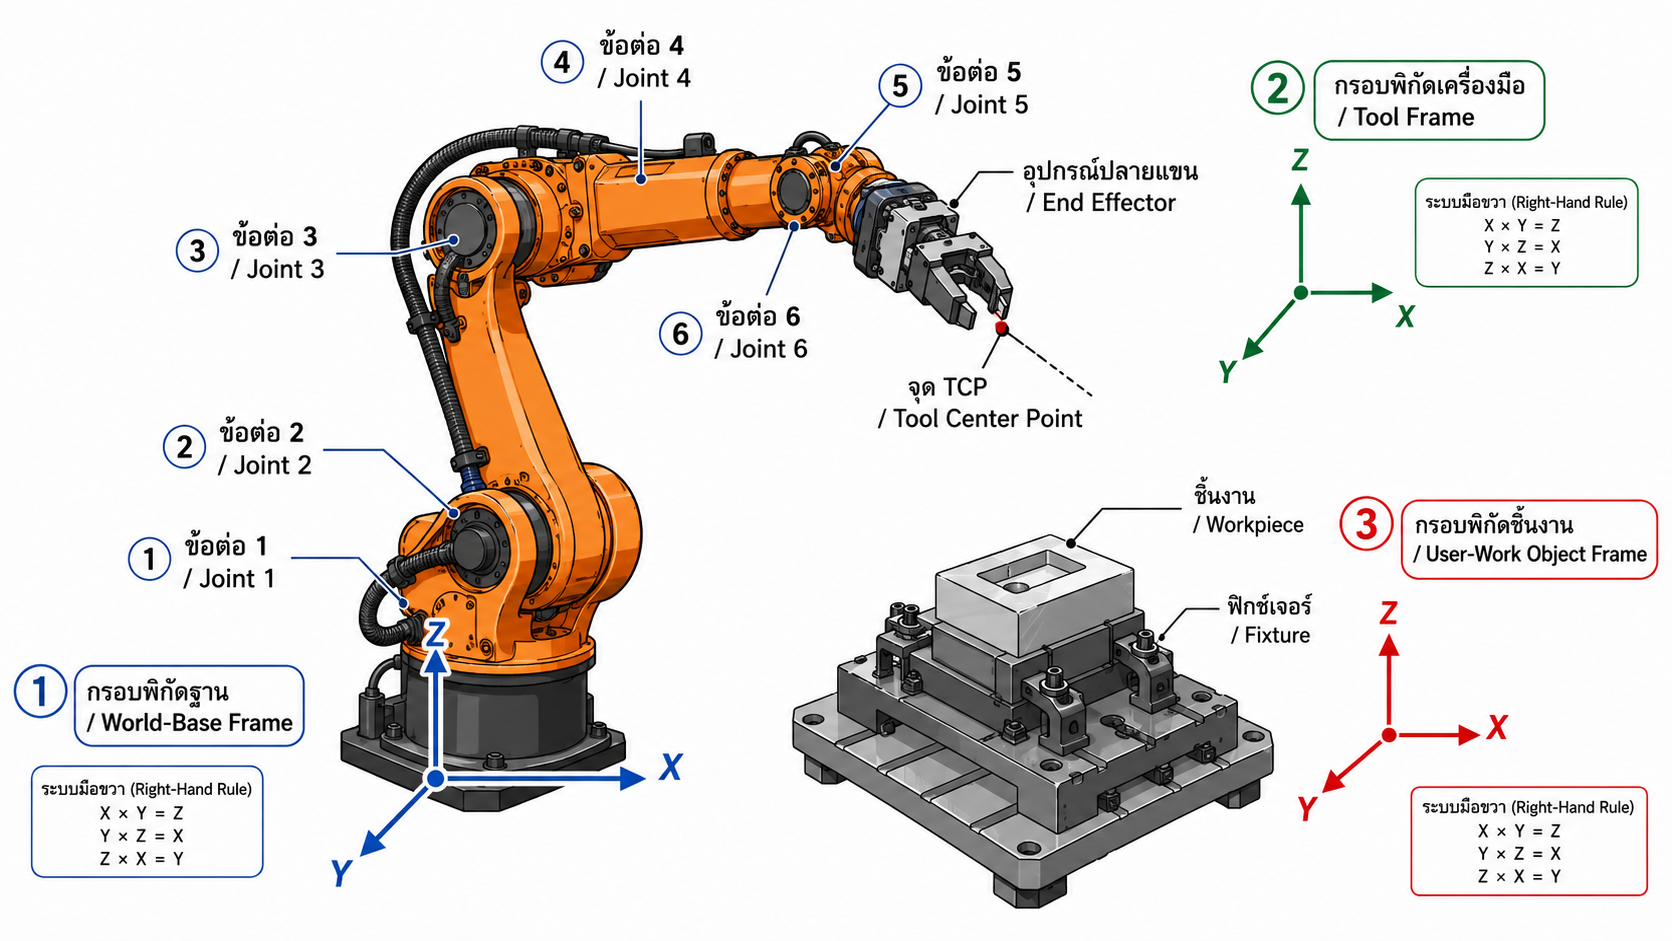
\includegraphics[width=0.8\textwidth]{images/chapter8/figure-01.png}
    \caption{ระบบพิกัด World, Tool และ User บนหุ่นยนต์ 6 แกน}
\end{figure}

\par\noindent\rule{\textwidth}{0.4pt}\par
\subsection{7.2 วิธีการสอนตำแหน่งหุ่นยนต์}

\subsubsection{7.2.1 Online Teaching ด้วย Teach Pendant}

Online Teaching คือการใช้ Controller และหุ่นยนต์จริงเพื่อสอนจุดหรือปรับโปรแกรมโดยตรง วิธีนี้ให้ข้อมูลจากระบบจริง เช่น Reachability, Joint Limit, Cable Routing, Fixture Clearance และพฤติกรรมของ End Effector แต่ทำให้เซลล์ไม่สามารถผลิตได้ในช่วงที่สอนและมีความเสี่ยงจากการเคลื่อนที่จริง

ลำดับการสอนตำแหน่งที่แนะนำมีดังนี้

\begin{enumerate}
    \item \textbf{ตรวจสอบพื้นที่และสถานะระบบ} — ไม่มีบุคคลหรือสิ่งของที่ไม่เกี่ยวข้องในพื้นที่ กำหนดผู้ควบคุม Teach Pendant เพียงคนเดียว
    \item \textbf{เลือก Operating Mode ที่เหมาะสม} — ใช้โหมด Manual/Teach แบบลดความเร็วตามข้อกำหนดของระบบฝึก
    \item \textbf{ตรวจสอบ Enabling Device} — ผู้สอนต้องเข้าใจตำแหน่งปล่อย กดกึ่งกลาง และกดสุดของอุปกรณ์
    \item \textbf{เลือก Tool และ User Frame} — ตรวจหมายเลข Tool/User ที่ Active ก่อน Jog
    \item \textbf{เลือก Coordinate System} — Joint, World, Tool หรือ User ตามเจตนาการเคลื่อนที่
    \item \textbf{เริ่มด้วยความเร็วต่ำ} — โดยเฉพาะเมื่ออยู่ใกล้ Fixture, Tool, Cable หรือ Singularity
    \item \textbf{Jog ไปยัง Approach Position} — ใช้จุดเหนือหรือห่างจากชิ้นงานก่อนเข้าสู่ตำแหน่งทำงาน
    \item \textbf{เข้าสู่ Work Position อย่างควบคุม} — ใช้ Tool หรือ User Coordinate เพื่อรักษาทิศทางที่เข้าใจง่าย
    \item \textbf{บันทึก Point} — ตั้งชื่อหรือหมายเลขให้สื่อความหมาย เช่น \texttt{P\_PICK\_APP}, \texttt{P\_PICK}, \texttt{P\_PLACE\_APP}
    \item \textbf{ตรวจสอบค่าที่บันทึก} — Frame, Tool, Configuration, Turn Number และ Motion Type
    \item \textbf{ทดสอบแบบ Step/Single Block} — เริ่มจากความเร็ว Override ต่ำและไม่มีชิ้นงาน
    \item \textbf{บันทึก Backup} — หลังการแก้โปรแกรมหรือ Frame ที่ผ่านการทวนสอบ
\end{enumerate}

\textbf{แนวคิด Approach–Process–Retreat}

การสอนจุดหนึ่งงานควรแยกอย่างน้อยเป็น 3 กลุ่ม

\begin{itemize}
    \item \textbf{Approach Point:} จุดปลอดภัยก่อนเข้าใกล้ชิ้นงาน
    \item \textbf{Process Point:} จุดที่ทำงานจริง เช่น Pick, Weld Start หรือ Inspection
    \item \textbf{Retreat Point:} จุดถอยออกจากชิ้นงานตามแนวที่ลดโอกาสชน
\end{itemize}

การใช้จุดเดียวทั้งเข้าและออกอาจเหมาะกับงานง่าย แต่ในงานที่มี Fixture ลึกหรือมีชิ้นส่วนยื่น การแยกจุดช่วยให้ Recovery และการวิเคราะห์ Collision ทำได้ชัดเจนกว่า

\subsubsection{7.2.2 Lead-through Programming}

Lead-through หรือ Hand Guiding คือการนำแขนหุ่นยนต์ด้วยมือในระบบที่ได้รับการออกแบบให้รองรับ เช่น Collaborative Robot หรือหุ่นยนต์ที่มีโหมด Hand Guiding และแรงชดเชยน้ำหนักจากผู้ผลิต การใช้งานทั่วไปประกอบด้วย

\begin{enumerate}
    \item เลือกโหมด Hand Guiding ที่ได้รับอนุญาต
    \item ตรวจสอบ Tool Payload, Center of Gravity และ TCP
    \item กดอุปกรณ์อนุญาตหรือปุ่ม Freedrive ตามระบบ
    \item นำ TCP ไปยัง Pose ที่ต้องการ
    \item บันทึก Waypoint หรือบันทึกเส้นทาง
    \item ปรับ Speed, Acceleration, Blend และ Orientation ในโปรแกรม
    \item จำลองหรือเล่นกลับที่ความเร็วต่ำ
\end{enumerate}

\textbf{ข้อจำกัดสำคัญ}

\begin{itemize}
    \item ไม่ใช่หุ่นยนต์ทุกชนิดที่อนุญาตให้ปลด Brake แล้วดึงแขนด้วยมือ
    \item การปลด Brake เพื่อ Service ไม่เท่ากับโหมด Hand Guiding สำหรับ Programming
    \item เส้นทางที่บันทึกด้วยมืออาจมี Noise จุดมากเกินไป หรือ Orientation ไม่สม่ำเสมอ
    \item ต้องประเมิน Pinch Point, Tool Hazard และแรงจาก Payload แม้เป็น Cobot
\end{itemize}

\subsubsection{7.2.3 Offline Programming}

Offline Programming (OLP) คือการสร้างโปรแกรม เส้นทาง และ Cell Layout บนคอมพิวเตอร์ โดยใช้ Robot Model และ Virtual Controller เมื่อเหมาะสม ตัวอย่างซอฟต์แวร์จากผู้ผลิต ได้แก่ FANUC ROBOGUIDE, ABB RobotStudio, KUKA.Sim หรือแพลตฟอร์มรุ่นใหม่ของ KUKA, Yaskawa MotoSim, Mitsubishi RT ToolBox3 และ Universal Robots URSim

\textbf{ขั้นตอน OLP ที่เป็นระบบ}

\begin{enumerate}
    \item นำเข้า CAD ของหุ่นยนต์ Fixture เครื่องจักร Tool และชิ้นงาน
    \item กำหนด Robot Base, External Axis และ Tool Geometry
    \item กำหนด TCP, Payload และ Work Object/User Frame
    \item สร้าง Targets และ Path
    \item เลือก Motion Type, Speed, Zone/Blend และ Process Parameters
    \item ตรวจ Reachability, Joint Limit, Singularity และ Collision
    \item ประมาณ Cycle Time
    \item สร้างหรือ Synchronize Program กับ Virtual Controller
    \item Export โปรแกรมตามรูปแบบที่ Controller รองรับ
    \item ทำ On-site Touch-up เพื่อชดเชยความคลาดเคลื่อนระหว่าง CAD กับระบบจริง
    \item ทดสอบใน Manual Reduced-speed ก่อน Automatic Mode
\end{enumerate}

\textbf{ข้อดี}

\begin{itemize}
    \item ลดเวลาที่ต้องหยุดสายการผลิต
    \item ตรวจ Collision และ Reachability ก่อนติดตั้งจริง
    \item ทดลอง Layout หลายทางเลือกได้
    \item ใช้สร้างสื่อการสอนและฝึกผู้เรียนโดยไม่เสี่ยงต่ออุปกรณ์จริง
    \item สนับสนุน Virtual Commissioning และการประเมิน Cycle Time
\end{itemize}

\textbf{ข้อจำกัด}

\begin{itemize}
    \item คุณภาพผลลัพธ์ขึ้นกับความถูกต้องของ CAD, Tool, Payload, Base และ Calibration
    \item Flexible Cable, Backlash, Thermal Drift และ Fixture Tolerance อาจไม่ถูกจำลองครบ
    \item Collision-free ใน Simulation ไม่ได้หมายความว่าปลอดภัยในระบบจริง
    \item Controller Option และ Software Version ต้องสอดคล้องกับหุ่นยนต์จริง
\end{itemize}

\subsubsection{ตาราง 8.3 เปรียบเทียบ Online, Lead-through และ Offline Programming}

\begin{table}[htbp]
    \centering
    \small
    \begin{tabularx}{\textwidth}{@{}L{0.17\textwidth}L{0.26\textwidth}L{0.28\textwidth}Y@{}}
        \hline
        \textbf{วิธี} & \textbf{จุดเด่น} & \textbf{ข้อจำกัด} & \textbf{งานที่เหมาะสม} \\
        \hline
        Teach Pendant & สอดคล้องกับระบบจริง เห็น Clearance จริง & ใช้เวลาหุ่นยนต์จริงและมีความเสี่ยง & Touch-up, Recovery, งานจุดไม่มาก \\
        Lead-through & เรียนรู้ง่าย เหมาะกับท่าทางเชิงสาธิต & ขึ้นกับรุ่นหุ่นยนต์และอาจได้เส้นทางไม่เรียบ & Cobot, งานสาธิต, งาน Path แบบง่าย \\
        Offline Programming & ลด Downtime ตรวจ Collision และ Cycle Time & ต้องมี Model และ Calibration ที่ดี & Welding, Painting, Machining, Cell ใหม่ \\
        \hline
    \end{tabularx}
\end{table}

\subsubsection{7.2.4 การกำหนดคุณภาพของจุดสอน}

จุดที่ดีไม่ได้หมายถึงเพียง TCP อยู่ตำแหน่งถูกต้อง แต่ต้องมีองค์ประกอบต่อไปนี้

\begin{itemize}
    \item Tool Frame และ User Frame ถูกต้อง
    \item Orientation เหมาะกับกระบวนการ
    \item Robot Configuration ไม่เปลี่ยนโดยไม่ตั้งใจ
    \item มีระยะเผื่อจาก Joint Limit และ Singularity
    \item สาย Tool และ Dress Pack ไม่บิดตึง
    \item Approach/Retreat ไม่ตัดผ่าน Fixture
    \item สามารถ Recover ได้เมื่อหยุดกลาง Cycle
    \item ชื่อ Point และ Comment สื่อความหมาย
    \item Point สำคัญที่ต้องสัมผัสชิ้นงานใช้ Fine/Exact Stop ตามความจำเป็น
    \item จุดผ่านที่ใช้เพิ่มความต่อเนื่องไม่ทำให้ Path เบี่ยงเข้าหาสิ่งกีดขวาง
\end{itemize}

\subsubsection{Checklist ก่อนบันทึกจุด}

\begin{verbatim}
[ ] Tool Number ถูกต้อง
[ ] User/Work Object Number ถูกต้อง
[ ] Coordinate System ตรงกับงาน
[ ] Speed Override อยู่ในระดับปลอดภัย
[ ] TCP และส่วนอื่นของแขนมี Clearance
[ ] Orientation ไม่ทำให้สายบิด
[ ] Joint อยู่ห่างจาก Limit และ Singularity
[ ] ตั้งชื่อ Point และ Comment แล้ว
[ ] กำหนด Motion Type และ Termination เหมาะสม
\end{verbatim}

\par\noindent\rule{\textwidth}{0.4pt}\par

\subsection{7.3 Motion Commands และการวางแผนเส้นทาง}

\subsubsection{7.3.1 ความแตกต่างระหว่าง Path และ Trajectory}

\begin{itemize}
    \item \textbf{Path} คือรูปร่างทางเรขาคณิตที่ TCP หรือ Joint เคลื่อนผ่าน โดยยังไม่ระบุเวลา
    \item \textbf{Trajectory} คือ Path ที่กำหนดเวลา ความเร็ว ความเร่ง และอาจรวม Jerk
\end{itemize}

โปรแกรมอาจกำหนดจุดต้นและจุดปลายเหมือนกัน แต่ให้ Trajectory ต่างกันจาก Motion Type, Speed, Acceleration, Payload และ Blending ดังนั้นการประเมินคุณภาพต้องพิจารณาทั้งตำแหน่งและพฤติกรรมตามเวลา

\subsubsection{7.3.2 Point-to-Point Motion: PTP}

PTP วางแผนการเคลื่อนที่ใน Joint Space โดยให้แต่ละ Joint เปลี่ยนจากค่าเริ่มต้นไปยังค่าปลาย หุ่นยนต์จะประสานเวลาให้แกนต่าง ๆ ถึงเป้าหมายตามแผนของ Controller รูปแบบเชิงแนวคิดเขียนได้เป็น

\[
q_i(t)=q_{i,0}+s(t)(q_{i,f}-q_{i,0})
\]

เมื่อ

\begin{itemize}
    \item $q_{i,0}$ คือค่าข้อต่อเริ่มต้น
    \item $q_{i,f}$ คือค่าข้อต่อปลาย
    \item $s(t)$ คือฟังก์ชันการเคลื่อนที่ที่เปลี่ยนจาก 0 เป็น 1
\end{itemize}

Controller จริงอาจใช้โปรไฟล์ความเร็วแบบ Trapezoidal, S-curve หรือวิธีเฉพาะของผู้ผลิต

\textbf{ข้อดี}

\begin{itemize}
    \item คำนวณได้มีประสิทธิภาพและมักเคลื่อนที่ได้เร็ว
    \item เหมาะสำหรับการเคลื่อนระหว่างจุดที่ไม่ต้องควบคุมรูปร่างเส้นทาง
    \item ใช้สำหรับ Home, Transfer หรือ Approach ที่มีพื้นที่ว่างเพียงพอ
\end{itemize}

\textbf{ข้อจำกัด}

\begin{itemize}
    \item เส้นทาง TCP ไม่รับประกันเป็นเส้นตรง
    \item ส่วนต่าง ๆ ของแขนอาจกวาดผ่านพื้นที่กว้าง
    \item ไม่เหมาะกับงานเชื่อม เดินกาว ตัด หรือพ่นที่ต้องควบคุม Path
\end{itemize}

ตัวอย่างคำสั่ง

\begin{verbatim}
FANUC: J P[1] 100% FINE
ABB:   MoveJ Target1, v1000, fine, tool1;
KUKA:  PTP P1
Yaskawa: MOVJ P001 VJ=50.00
URScript: movej(q_target, a=1.2, v=0.8)
\end{verbatim}

\begin{quote}
รูปแบบคำสั่งเป็นตัวอย่างเชิงการเรียนรู้ ต้องตรวจ Syntax, Unit และ Option จากคู่มือ Controller รุ่นที่ใช้งาน
\end{quote}

\subsubsection{7.3.3 Linear Motion: LIN}

Linear Motion ควบคุมให้ TCP เคลื่อนตามเส้นตรงจากตำแหน่งเริ่ม $\mathbf{p}_0$ ไปยังตำแหน่งปลาย $\mathbf{p}_f$

\[
\mathbf{p}(t)=\mathbf{p}_0+s(t)(\mathbf{p}_f-\mathbf{p}_0)
\]

Controller ต้องคำนวณ Inverse Kinematics หลายครั้งตามเส้นทาง เพื่อหาค่า Joint ที่ทำให้ TCP อยู่บนเส้นตรงและ Orientation เปลี่ยนตามกฎที่กำหนด

\textbf{เหมาะสำหรับ}

\begin{itemize}
    \item เข้า–ออกชิ้นงานตามแนว Tool
    \item งานเชื่อมแนวตรง เดินกาว ตัด และตรวจสอบ
    \item งานหยิบวางที่ต้องหลีกเลี่ยงขอบ Fixture
    \item การเคลื่อนชิ้นงานที่ต้องรักษาระดับหรือ Orientation
\end{itemize}

\textbf{ข้อจำกัด}

\begin{itemize}
    \item อาจผ่าน Singularity หรือ Joint Limit แม้จุดต้นและปลายเข้าถึงได้
    \item ความเร็ว TCP สูงอาจต้องการความเร็ว Joint สูงมากในบางท่าทาง
    \item ใช้ทรัพยากรการคำนวณและข้อจำกัดของ Controller มากกว่า PTP
\end{itemize}

\begin{verbatim}
FANUC: L P[2] 500mm/sec FINE
ABB:   MoveL Target2, v500, z10, tool1;
KUKA:  LIN P2
Yaskawa: MOVL P002 V=500.0
URScript: movel(p_target, a=0.5, v=0.25)
\end{verbatim}

\subsubsection{7.3.4 Circular Motion: CIRC/ARC}

การเคลื่อนที่เป็นวงโค้งต้องมีอย่างน้อยจุดเริ่ม จุดผ่าน และจุดปลาย เพื่อกำหนดระนาบและส่วนโค้ง

\begin{verbatim}
FANUC: C P[3] P[4] 500mm/sec FINE
ABB:   MoveC CirPoint, Target3, v500, z10, tool1;
KUKA:  CIRC P3, P4
Yaskawa: MOVC P003 V=300.0
URScript: movec(p_via, p_to, a=0.5, v=0.2)
\end{verbatim}

\textbf{การประยุกต์ใช้} ได้แก่ การเชื่อมตามท่อ งานขัดขอบโค้ง งานพ่นสี และการเคลื่อนรอบชิ้นงานทรงกระบอก

\textbf{ข้อควรระวัง}

\begin{itemize}
    \item จุดทั้งสามต้องไม่เกือบอยู่บนเส้นตรงเดียวกัน
    \item Orientation ระหว่างจุดต้องถูกกำหนดให้เหมาะสมกับกระบวนการ
    \item หาก Arc ใหญ่หรือซับซ้อน ควรแบ่งเป็นหลายส่วนและตรวจ Continuity
\end{itemize}

\subsubsection{7.3.5 Blending, Zone และ CNT}

หากกำหนดจุดเป็น Fine/Exact Stop หุ่นยนต์จะลดความเร็วจนเข้าเกณฑ์ตำแหน่งก่อนเริ่ม Motion ถัดไป การหยุดทุกจุดเพิ่ม Cycle Time และทำให้ความเร่งเปลี่ยนบ่อย ในทางกลับกัน Blending ทำให้ Controller เริ่มเบี่ยงจากจุดเดิมเพื่อเชื่อมกับเส้นทางถัดไปอย่างต่อเนื่อง

\begin{table}[htbp]
    \centering
    \begin{tabular}{l l r r}
        \hline
        \textbf{ค่าตัวอย่าง} & \textbf{พฤติกรรมโดยแนวคิด} & \textbf{ผลต่อ Cycle Time} & \textbf{ผลต่อความแม่นยำผ่านจุด} \\
        \hline
        FINE / fine & เข้าเป้าหมายตามเกณฑ์แล้วจึงไปต่อ & สูง & สูง \\
        CNT 0 หรือ Zone ใกล้ศูนย์ & เกือบหยุดหรือเบี่ยงน้อย & ค่อนข้างสูง & ค่อนข้างสูง \\
        CNT 50 / Zone ปานกลาง & กลมมุมระดับกลาง & ลดลง & จุดผ่านคลาดมากขึ้น \\
        CNT 100 / Zone ใหญ่ & ต่อเนื่องสูง เบี่ยงจากจุดมาก & ต่ำ & ไม่เหมาะกับจุดกระบวนการสำคัญ \\
        \hline
    \end{tabular}
\end{table}

\textbf{หลักการเลือก}

\begin{itemize}
    \item จุด Pick, Place, Tool Change, Probe และจุดที่รอสัญญาณควรใช้ Fine หรือ Zone ต่ำ
    \item จุดผ่านกลางอากาศที่มี Clearance มากอาจใช้ Blend สูง
    \item ห้ามเพิ่ม Blend โดยดูเฉพาะ Cycle Time ต้องตรวจ Swept Volume ของ TCP และทุก Link
    \item Path ที่มุมแหลมมากอาจไม่สามารถรักษาความเร็วคงที่ได้ แม้กำหนด Blend
\end{itemize}

\subsubsection{ตัวอย่างที่ 8.2 ผลของการหยุดต่อ Cycle Time}

\textbf{ตัวอย่างเพิ่มเติมเพื่อการเรียนรู้}

โปรแกรมมีจุดผ่านกลางอากาศ 4 จุด หากใช้ Fine ทุกจุด หุ่นยนต์ใช้เวลาเร่งและลดความเร็วเพิ่มจุดละ 0.25 s เมื่อเปลี่ยนจุดผ่านทั้ง 4 เป็น Blend ที่ผ่านการตรวจ Collision แล้ว จะลดเวลาได้โดยประมาณเท่าใด

\[
\Delta t = 4(0.25)=1.00\text{ s/cycle}
\]

ถ้าผลิต 3,600 Cycle ต่อวัน เวลาที่ลดได้คือ

\[
1.00\times 3600=3600\text{ s}=60\text{ min/day}
\]

\textbf{การแปลความหมาย:} การปรับ Motion Termination ที่จุดไม่สำคัญสามารถเพิ่มกำลังการผลิตได้มาก แต่ต้องยืนยันว่า Path ใหม่ไม่เข้าใกล้คน อุปกรณ์ หรือชิ้นงานเกินเกณฑ์

\subsubsection{7.3.6 ปัจจัยที่มีผลต่อ Path Planning}

\begin{enumerate}
    \item \textbf{Reachability:} จุดต้องอยู่ใน Working Envelope และไม่เกิน Joint Limit
    \item \textbf{Robot Configuration:} Shoulder, Elbow, Wrist และ Turn Number ต้องสอดคล้องตลอดเส้นทาง
    \item \textbf{Singularity:} ควรหลีกเลี่ยงท่าที่ต้องการความเร็ว Joint สูงผิดปกติ
    \item \textbf{Payload และ Center of Gravity:} มีผลต่อ Acceleration, Braking และ Alarm Overload
    \item \textbf{Tool Geometry:} ต้องตรวจทั้ง TCP และ Volume ของ Tool
    \item \textbf{Dress Pack:} สายไฟ สายลม และสายเชื่อมต้องไม่ตึงหรือเสียดสี
    \item \textbf{Fixture Clearance:} ต้องรวม Tolerance, Deflection และตำแหน่งชิ้นงานจริง
    \item \textbf{Process Requirement:} งานเชื่อมและพ่นต้องควบคุม Speed และ Orientation ต่อเนื่อง
    \item \textbf{Recovery:} ต้องมีจุดหรือขั้นตอนถอยออกเมื่อ Cycle หยุดกลางทาง
    \item \textbf{Safety Zone:} เส้นทางต้องอยู่ภายในข้อจำกัดของ Safety Function และพื้นที่อนุญาต
\end{enumerate}

\subsubsection{ตาราง 8.4 แนวทางเลือก Motion ตามงาน}

\begin{table}[htbp]
    \centering
    \begin{tabular}{l l l l}
        \hline
        \textbf{สถานการณ์} & \textbf{Motion แนะนำ} & \textbf{Termination} & \textbf{เหตุผล} \\
        \hline
        เคลื่อนจาก Home ไปเหนือจุด Pick & PTP/J & Blend ปานกลางเมื่อมี Clearance & ลด Cycle Time \\
        ลงจับชิ้นงานใน Fixture & Linear & Fine & รักษาแนวเข้าและตำแหน่งจับ \\
        ถอย Gripper ออกจากชิ้นงาน & Linear & Blend ต่ำหรือ Fine & ลดการเฉี่ยวชิ้นงาน \\
        เคลื่อนระหว่างพื้นที่ว่าง & PTP/J & Blend สูงตามการตรวจสอบ & เร็วและใช้เส้นทาง Joint \\
        เชื่อมแนวตรง & Linear & Zone ต่อเนื่องตาม Process & รักษาความเร็วและแนวเชื่อม \\
        เชื่อมแนวโค้ง & Circular & Zone ที่ไม่ทำลายรูปทรง & รักษา Arc และความต่อเนื่อง \\
        เข้า Tool Changer & Linear & Fine & ต้องจัดแนวและล็อกอย่างแม่นยำ \\
        \hline
    \end{tabular}
\end{table}

% [รูปที่ 8.2: เปรียบเทียบเส้นทาง PTP และ Linear]
% ประเภทภาพ: Technical Illustration
% ตำแหน่งที่แนะนำ: หลังหัวข้อ 7.3.3
% วัตถุประสงค์การเรียนรู้: ให้เห็นว่า PTP ไม่รับประกันเส้นทาง TCP ขณะที่ LIN ควบคุมเส้นตรง
% คำอธิบายภาพ: จุด A และ B เดียวกัน มีเส้นโค้งของ TCP สำหรับ PTP และเส้นตรงสำหรับ LIN พร้อมภาพท่าหุ่นยนต์ระหว่างทาง
% องค์ประกอบที่ต้องมี: Robot poses, Point A, Point B, curved PTP path, straight LIN path, obstacle clearance
% ข้อความหรือป้ายกำกับ: PTP/Joint-space, LIN/Cartesian straight line
% ภาษาของป้ายกำกับ: ไทยและอังกฤษ
% สัดส่วนภาพ: 16:9
% Image Generation Prompt: Clean engineering textbook comparison of a six-axis industrial robot moving between the same point A and point B. Left panel shows point-to-point joint-space motion with a curved and uncontrolled TCP path. Right panel shows linear Cartesian motion with a straight TCP path. Include intermediate robot poses, an obstacle for clearance context, arrows and bilingual Thai-English labels. White background, precise vector style, 16:9.
% Alt Text: ภาพเปรียบเทียบเส้นทาง TCP แบบโค้งของ PTP กับเส้นตรงของ Linear Motion

\begin{figure}[htbp]
    \centering
    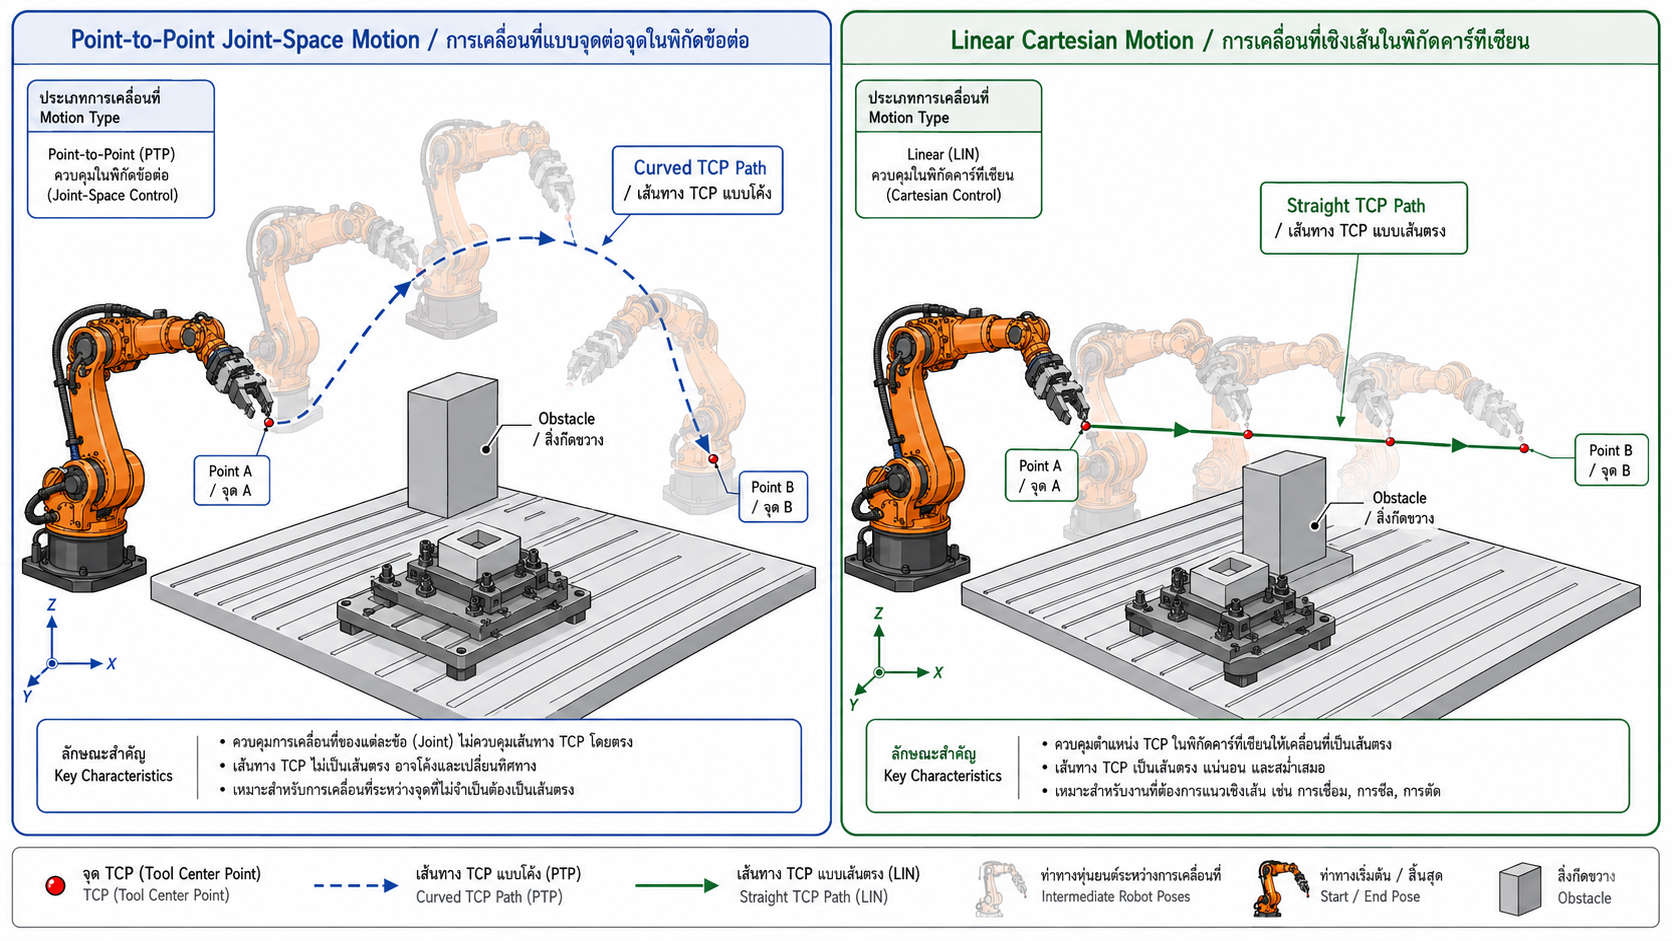
\includegraphics[width=0.8\textwidth]{images/chapter8/figure-02.png}
    \caption{เปรียบเทียบเส้นทาง PTP และ Linear}
\end{figure}

% [รูปที่ 8.3: ผลของ FINE และ CNT/Zone Blending]
% ประเภทภาพ: Technical Diagram
% ตำแหน่งที่แนะนำ: หลังหัวข้อ 7.3.5
% วัตถุประสงค์การเรียนรู้: แสดงการเบี่ยงจากจุดผ่านเมื่อเพิ่มระดับ Blending
% คำอธิบายภาพ: เส้นทางหักมุมผ่าน P1–P2–P3 เปรียบเทียบ FINE, Blend ต่ำ, Blend กลาง และ Blend สูง
% องค์ประกอบที่ต้องมี: จุด P1 P2 P3, exact path, four rounded paths, deviation distance and velocity arrows
% ข้อความหรือป้ายกำกับ: FINE, CNT/Zone Low, Medium, High, Path Deviation
% ภาษาของป้ายกำกับ: ไทยและอังกฤษ
% สัดส่วนภาพ: 16:9
% Image Generation Prompt: Engineering path diagram showing a robot TCP moving through three points P1, P2 and P3 with a sharp corner at P2. Compare four trajectories: FINE exact stop, low blend, medium blend and high blend. Show increasing corner radius, path deviation and smoother velocity continuity. Clean white background, precise vector lines, bilingual Thai-English labels, 16:9.
% Alt Text: เส้นทางผ่านสามจุดที่มีการกลมมุมเพิ่มขึ้นจาก FINE ไปยัง Blend สูง

\begin{figure}[htbp]
    \centering
    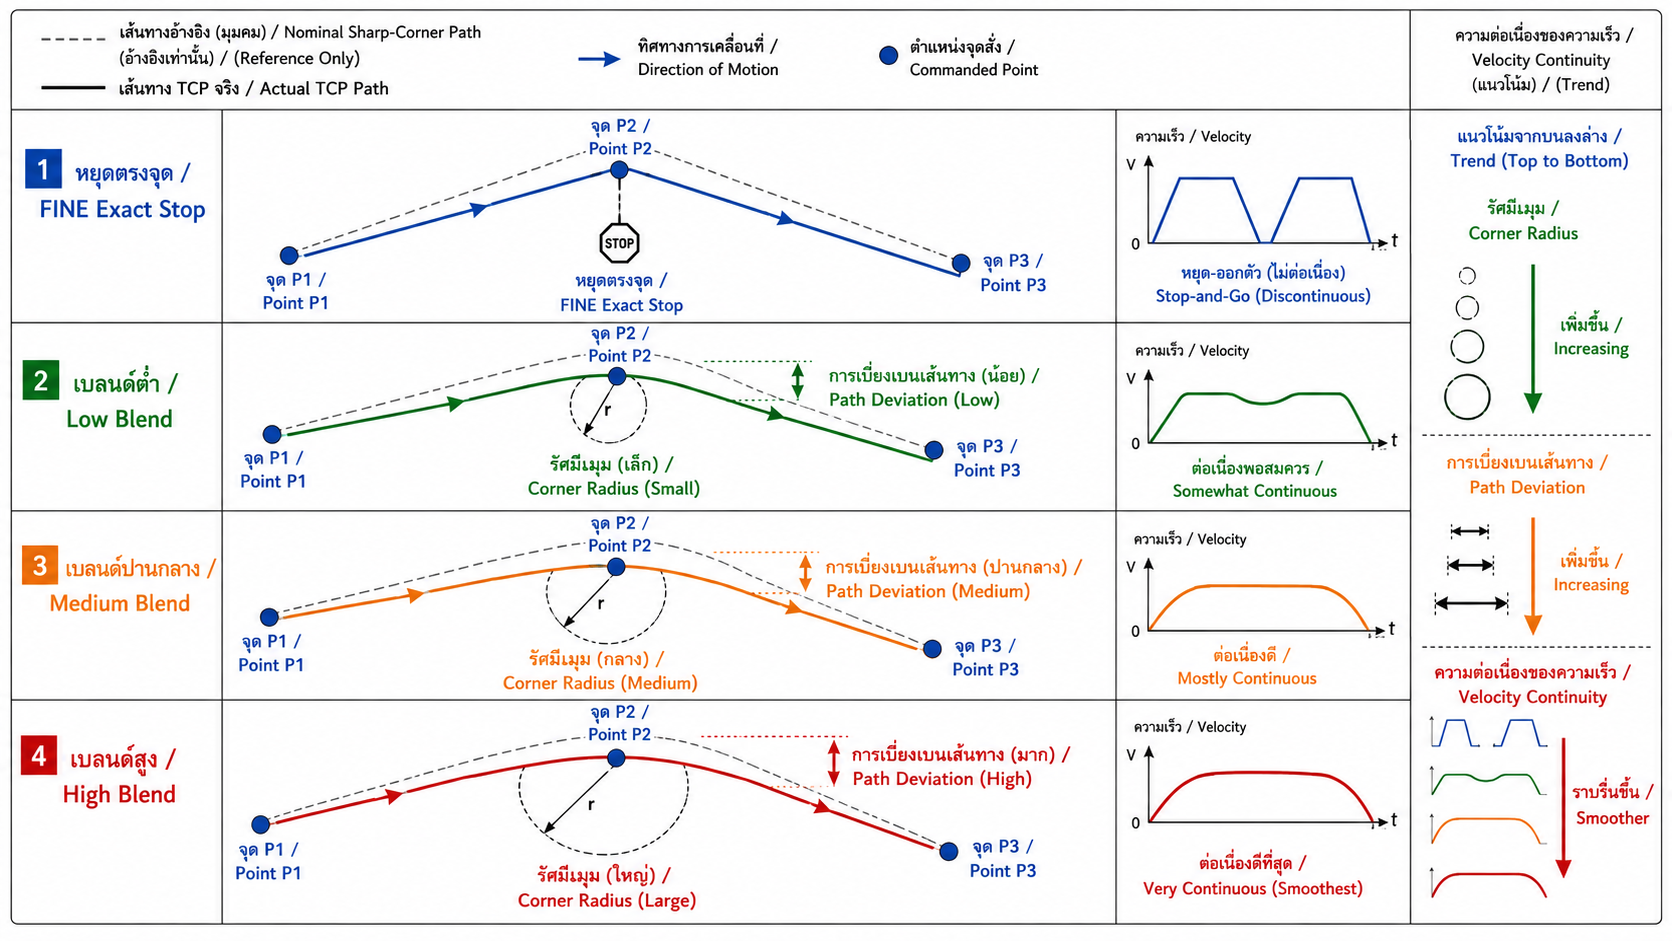
\includegraphics[width=0.8\textwidth]{images/chapter8/figure-03.png}
    \caption{ผลของ FINE และ CNT/Zone Blending}
\end{figure}

\par\noindent\rule{\textwidth}{0.4pt}\par

\subsection{7.4 โครงสร้างโปรแกรมหุ่นยนต์เบื้องต้น}

\subsubsection{7.4.1 องค์ประกอบของโปรแกรมที่อ่านและบำรุงรักษาได้}

โปรแกรมหุ่นยนต์ที่ดีควรแยกองค์ประกอบต่อไปนี้

\begin{enumerate}
    \item \textbf{Configuration:} หมายเลข Tool, User Frame, Payload, Speed Override และ Process Mode
    \item \textbf{Position Data:} Home, Approach, Process, Retreat, Recovery และ Maintenance Position
    \item \textbf{Motion Logic:} ลำดับ J/L/C หรือ MoveJ/MoveL/MoveC
    \item \textbf{I/O Logic:} Gripper, Clamp, Sensor, Conveyor, Machine Ready และ Safety-permissive interface
    \item \textbf{Control Flow:} IF, SELECT, LOOP, FOR, CALL, WAIT, TIMER และ Label
    \item \textbf{Fault Handling:} Timeout, Retry Limit, Alarm Message และ Safe Stop
    \item \textbf{Production Data:} Counter, Recipe, Part Type และ Result
    \item \textbf{Comments and Revision:} ผู้แก้ไข วันที่ เหตุผล และ Version
\end{enumerate}

\subsubsection{7.4.2 ตัวอย่างโปรแกรม Pick and Place แบบ FANUC TP-like}

\begin{verbatim}
1:  !--- PICK AND PLACE PROGRAM --- ;
2:  UFRAME_NUM=1 ;
3:  UTOOL_NUM=1 ;
4:  ! Verify cell conditions ;
5:  WAIT DI[1:CELL_READY]=ON ;
6:  WAIT DI[2:PART_PRESENT]=ON ;
7:  WAIT DI[3:PLACE_CLEAR]=ON ;
8:  ;
9:  !--- HOME POSITION --- ;
10: J P[1:HOME] 50% FINE ;
11: ;
12: !--- APPROACH PICK --- ;
13: J P[2:PICK_APP] 50% CNT50 ;
14: L P[3:PICK] 150mm/sec FINE ;
15: DO[1:GRIP_CLOSE]=ON ;
16: WAIT DI[4:GRIP_OK]=ON TIMEOUT,LBL[900] ;
17: L P[2:PICK_APP] 200mm/sec CNT20 ;
18: ;
19: !--- MOVE TO PLACE --- ;
20: J P[4:PLACE_APP] 50% CNT50 ;
21: L P[5:PLACE] 150mm/sec FINE ;
22: DO[1:GRIP_CLOSE]=OFF ;
23: WAIT DI[5:GRIP_OPEN]=ON TIMEOUT,LBL[910] ;
24: L P[4:PLACE_APP] 200mm/sec CNT20 ;
25: J P[1:HOME] 50% FINE ;
26: DO[2:CYCLE_COMPLETE]=ON ;
27: WAIT 0.10(sec) ;
28: DO[2:CYCLE_COMPLETE]=OFF ;
29: END ;
30: ;
31: LBL[900] ;
32: CALL GRIP_FAULT ;
33: END ;
34: LBL[910] ;
35: CALL RELEASE_FAULT ;
36: END ;
\end{verbatim}

\begin{quote}
โค้ดนี้เป็นตัวอย่างเพื่ออธิบายโครงสร้าง ไม่ใช่ไฟล์ที่รับรองว่าสามารถโหลดได้กับ Controller ทุก Version ชื่อคำสั่ง Timeout และรูปแบบ Label ต้องปรับตามคู่มือจริง
\end{quote}

\subsubsection{7.4.3 ลำดับ Handshake กับ PLC}

การเชื่อมต่อหุ่นยนต์กับ PLC ควรใช้ State หรือ Handshake ที่ตรวจสอบได้ ไม่ควรใช้ Pulse สั้นโดยไม่มีการยืนยัน ตัวอย่างสัญญาณ ได้แก่

\begin{table}[htbp]
    \centering
    \begin{tabular}{l l}
        \hline
        \textbf{สัญญาณจาก PLC ไป Robot} & \textbf{ความหมาย} \\
        \hline
        \texttt{CELL\_READY} & อุปกรณ์รอบเซลล์อยู่ในสถานะพร้อม \\
        \texttt{START\_REQUEST} & ขอให้หุ่นยนต์เริ่ม Cycle \\
        \texttt{PART\_PRESENT} & มีชิ้นงานที่จุด Pick \\
        \texttt{PLACE\_CLEAR} & ตำแหน่งวางว่างและปลอดภัย \\
        \texttt{RESET\_REQUEST} & ขอ Reset หลังเงื่อนไขปลอดภัยครบ \\
        \hline
    \end{tabular}
\end{table}

\begin{table}[htbp]
    \centering
    \begin{tabular}{l l}
        \hline
        \textbf{สัญญาณจาก Robot ไป PLC} & \textbf{ความหมาย} \\
        \hline
        \texttt{ROBOT\_READY} & Robot อยู่ Home/Ready และไม่มี Fault \\
        \texttt{ROBOT\_BUSY} & กำลังทำ Cycle \\
        \texttt{CYCLE\_COMPLETE} & Cycle สำเร็จ \\
        \texttt{ROBOT\_FAULT} & มี Fault ต้องดำเนินการ \\
        \texttt{GRIP\_RESULT} & ผลการจับชิ้นงาน \\
        \hline
    \end{tabular}
\end{table}

ตัวอย่าง Sequence

\begin{verbatim}
PLC: START_REQUEST = ON
Robot: ตรวจ CELL_READY, PART_PRESENT, PLACE_CLEAR
Robot: ROBOT_BUSY = ON
Robot: ทำ Pick and Place
Robot: CYCLE_COMPLETE = ON
PLC: START_REQUEST = OFF และรับ Complete
Robot: CYCLE_COMPLETE = OFF, ROBOT_BUSY = OFF
\end{verbatim}

การออกแบบต้องกำหนดพฤติกรรมเมื่อสัญญาณค้าง สัญญาณหายระหว่าง Cycle หรือ Controller Restart เพื่อป้องกันการเริ่มซ้ำโดยไม่ตั้งใจ

\subsubsection{7.4.4 โครงสร้างควบคุมการไหล}

\begin{verbatim}
!--- IF CONDITION ---
IF DI[1:PART_OK] = ON THEN
  CALL PICK_ROUTINE
ELSE
  CALL EJECT_ROUTINE
ENDIF

!--- FOR LOOP ---
FOR R[1:INDEX] = 1 TO 10
  CALL CYCLE_ROUTINE
  R[2:GOOD_COUNT] = R[2:GOOD_COUNT] + 1
ENDFOR

!--- WAIT WITH TIMEOUT ---
WAIT DI[2:CLAMP_OK] = ON TIMEOUT LBL[100]
\end{verbatim}

\textbf{ข้อควรระวังของ Loop}

\begin{itemize}
    \item ต้องมีเงื่อนไขออกจาก Loop ที่ตรวจสอบได้
    \item ไม่ควร Retry การจับชิ้นงานไม่จำกัดครั้ง
    \item Counter ต้องถูก Initial เมื่อเริ่ม Lot หรือหลัง Recovery ตามกติกาที่ชัดเจน
    \item การ Restart ต้องรู้ว่า Cycle อยู่ State ใด ไม่ควรกลับไปเริ่มต้นโดยอัตโนมัติทุกกรณี
\end{itemize}

\subsubsection{7.4.5 ตัวอย่างโปรแกรมวางชิ้นงาน 2 × 5 ช่องแบบ Pseudocode}

\begin{verbatim}
SET ROWS = 2
SET COLS = 5
SET PITCH_X = 40 mm
SET PITCH_Y = 60 mm

FOR row = 0 TO ROWS-1
  FOR col = 0 TO COLS-1
    WAIT part_present = TRUE
    CALL PickPart()

    IF gripper_confirm = FALSE THEN
      RAISE "GRIPPER NOT CONFIRMED"
      STOP CYCLE
    ENDIF

    target = tray_origin
             + col * PITCH_X along User-X
             + row * PITCH_Y along User-Y

    MoveJ target_approach WITH blend
    MoveL target WITH fine
    OpenGripper()
    WAIT gripper_open = TRUE WITH timeout
    MoveL target_approach WITH low_blend
  ENDFOR
ENDFOR
\end{verbatim}

จุดเด่นของแนวทางนี้คือใช้จุดต้นเพียงจุดเดียวร่วมกับ Offset จึงลดจำนวน Point และทำให้ปรับ Pitch ได้ง่าย แต่ต้องตรวจว่า Offset ทุกจุดอยู่ใน Reach, ไม่เกิด Singularity และไม่ชนขอบถาด

\subsubsection{7.4.6 การจัดการ Timeout และ Fault}

การใช้ \texttt{WAIT} โดยไม่มี Timeout อาจทำให้โปรแกรมค้างโดยไม่ทราบสาเหตุ แนวทางที่ดีกว่าคือ

\begin{enumerate}
    \item เริ่ม Timer เมื่อส่งคำสั่งไปยังอุปกรณ์
    \item รอสัญญาณตอบกลับภายในเวลาที่กำหนด
    \item หากครบเวลา ให้หยุด Sequence ที่ปลอดภัย
    \item ปิด Output ที่อาจทำให้เกิดการเคลื่อนที่ต่อ
    \item แสดง Alarm ที่ระบุอุปกรณ์และ State
    \item ให้ผู้ปฏิบัติงานตรวจสาเหตุ
    \item อนุญาต Retry เมื่อเงื่อนไขปลอดภัยครบและจำนวนครั้งไม่เกินกำหนด
    \item บันทึกเหตุการณ์เพื่อวิเคราะห์ซ้ำ
\end{enumerate}

\subsubsection{7.4.7 การตรวจสอบโปรแกรมก่อนใช้งานจริง}

\textbf{ระดับที่ 1: Static Review}

\begin{itemize}
    \item Tool/User Frame ถูกต้อง
    \item Point Name และ Comment ชัดเจน
    \item Speed และ Termination เหมาะสม
    \item I/O Address ไม่ซ้ำหรือกลับ Logic
    \item Timeout และ Fault Path ครบ
    \item ไม่มี Jump/Label ที่ทำให้ข้าม Interlock
\end{itemize}

\textbf{ระดับที่ 2: Simulation}

\begin{itemize}
    \item Reachability และ Joint Limit
    \item Collision ของ Robot, Tool, Workpiece และ Fixture
    \item Cycle Time และ Bottleneck
    \item Singularity และ Configuration Change
\end{itemize}

\textbf{ระดับที่ 3: Dry Run บนหุ่นยนต์จริง}

\begin{itemize}
    \item ใช้ Manual Reduced-speed และ Step Mode
    \item ไม่มีชิ้นงานหรือใช้ชิ้นงานจำลองที่ปลอดภัย
    \item ผู้ควบคุมถือ Teach Pendant และสังเกต Clearance
    \item ตรวจทิศทาง Gripper/Actuator ก่อนจ่ายพลังงานเต็ม
\end{itemize}

\textbf{ระดับที่ 4: Process Validation}

\begin{itemize}
    \item ทดสอบด้วยชิ้นงานจริงภายใต้การควบคุม
    \item วัดคุณภาพ ตำแหน่ง Cycle Time และ Repeatability
    \item ทดสอบ Fault Scenario ที่ได้รับอนุญาต
    \item บันทึก Version และ Backup หลังอนุมัติ
\end{itemize}

\par\noindent\rule{\textwidth}{0.4pt}\par
\subsection{7.5 การบำรุงรักษาหุ่นยนต์อุตสาหกรรม}

\subsubsection{7.5.1 เป้าหมายของการบำรุงรักษา}

การบำรุงรักษาไม่ได้มีเป้าหมายเพียง “ซ่อมให้กลับมาทำงาน” แต่ต้องรักษาคุณลักษณะสำคัญของระบบ ได้แก่

\begin{itemize}
    \item ความปลอดภัยของผู้ปฏิบัติงาน
    \item ความพร้อมใช้งานของเซลล์
    \item ความแม่นยำและ Repeatability
    \item คุณภาพของกระบวนการ
    \item อายุของ Gear, Bearing, Brake, Cable และ Seal
    \item ความสมบูรณ์ของ Backup, Calibration และ Safety Configuration
    \item ความสามารถในการติดตามประวัติและวิเคราะห์สาเหตุซ้ำ
\end{itemize}

ประเภทการบำรุงรักษาที่พบ ได้แก่

\begin{enumerate}
    \item \textbf{Corrective Maintenance:} ซ่อมหลังเกิดความขัดข้อง
    \item \textbf{Preventive Maintenance:} ทำตามเวลา ชั่วโมงทำงาน หรือจำนวน Cycle
    \item \textbf{Condition-based Maintenance:} ทำเมื่อข้อมูลสภาพ เช่น อุณหภูมิ กระแสมอเตอร์ การสั่น หรือ Alarm Trend เปลี่ยน
    \item \textbf{Predictive Maintenance:} ใช้ข้อมูลและแบบจำลองคาดการณ์แนวโน้มความเสียหายก่อนหยุดเครื่อง
\end{enumerate}

ในห้องปฏิบัติการควรเน้น Preventive Maintenance และการตรวจสภาพพื้นฐาน ส่วนงาน Predictive Maintenance อาจสาธิตด้วยข้อมูล Trend หรือซอฟต์แวร์ Monitoring โดยไม่ดัดแปลงระบบจริง

\subsubsection{7.5.2 หลักการสร้างแผน PM}

แผน PM ที่ดีต้องตอบคำถาม 6 ข้อ

\begin{enumerate}
    \item \textbf{ตรวจอะไร} — เช่น Cable, Grease Leakage, Bolt, Fan, Filter, Battery และ Safety Device
    \item \textbf{ตรวจเมื่อใด} — รายวัน รายสัปดาห์ รายเดือน รายปี ชั่วโมงทำงาน หรือ Condition-based
    \item \textbf{ตรวจอย่างไร} — Visual, Torque Check, Functional Test, Measurement หรือ Trend Analysis
    \item \textbf{เกณฑ์ผ่านคืออะไร} — Normal/Abnormal, ค่าพิกัด, Tolerance หรือคำแนะนำผู้ผลิต
    \item \textbf{ใครรับผิดชอบ} — Operator, Maintenance Technician, Safety Specialist หรือผู้ผลิต
    \item \textbf{บันทึกที่ใด} — Checklist, CMMS, Logbook หรือระบบ Digital Maintenance
\end{enumerate}

\begin{quote}
\textbf{ข้อควรระวัง:} ระยะเปลี่ยน Grease, Battery, Belt, Seal และ Oil แตกต่างกันมากตามรุ่น ชั่วโมงทำงาน โหลด อุณหภูมิ และสภาพแวดล้อม ตารางต่อไปนี้เป็นโครงสร้างตัวอย่างเพื่อการเรียนรู้ ไม่ใช่คำสั่งบำรุงรักษาแทนคู่มือผู้ผลิต
\end{quote}

\subsubsection{ตาราง 8.5 แผน Preventive Maintenance ตัวอย่าง}

\begin{table}[htbp]
    \centering
    \small
    \begin{tabularx}{\textwidth}{@{}L{0.15\textwidth}L{0.20\textwidth}YL{0.19\textwidth}@{}}
        \hline
        \textbf{ความถี่ตัวอย่าง} & \textbf{กิจกรรม} & \textbf{รายละเอียดและเกณฑ์เบื้องต้น} & \textbf{ผู้รับผิดชอบ} \\
        \hline
        ก่อนเริ่มงานทุกวัน & Daily Visual Check & ตรวจรอยรั่ว Cable Damage ฝาครอบหลวม Tool หลวม เสียงผิดปกติ Air Pressure และ Alarm ค้าง & Operator \\
        ทุกสัปดาห์ & Functional Check & ทดสอบ Gripper Sensor, Interlock, Indicator และทำความสะอาดพื้นที่โดยไม่รบกวนอุปกรณ์นิรภัย & Operator/Technician \\
        ทุก 1–3 เดือน & Condition Inspection & ตรวจ Connector, Dress Pack, Fan/Filter, Bolt Mark, Backlash ที่สังเกตได้ และแนวโน้ม Alarm & Technician \\
        ตามชั่วโมงหรือคู่มือ & Lubrication Service & ใช้ชนิด ปริมาณ ตำแหน่ง และวิธีเติมตามคู่มือรุ่นนั้น ห้ามผสม Grease โดยไม่ยืนยันความเข้ากันได้ & Qualified Technician \\
        ทุกปีหรือรอบที่กำหนด & Annual Inspection & ตรวจ Brake, Cable, Safety Function, Calibration Status, Backup, Battery Condition และ Mechanical Wear & Qualified Technician \\
        ตามอายุ/สถานะ & Encoder/SMB Battery & เปลี่ยนตามคู่มือและขั้นตอนรักษาข้อมูลตำแหน่ง ห้ามตัดไฟผิดวิธี & Qualified Technician \\
        หลัง Crash/Repair & Re-mastering and Validation & ตรวจ Mastering, TCP, User Frame, Accuracy, Safety Zone และทดลองเส้นทาง & Engineer/Integrator \\
        Major Service & Gearbox/Wrist/Reducer Service & ดำเนินการตามคู่มือหรือศูนย์บริการ เนื่องจากต้องใช้เครื่องมือและวิธีเฉพาะ & Manufacturer/Authorized Service \\
        \hline
    \end{tabularx}
\end{table}

\subsubsection{7.5.3 Daily Check}

รายการตรวจประจำวันควรสั้น ชัดเจน และทำได้ก่อนเริ่มผลิต ตัวอย่าง

\begin{verbatim}
[ ] ไม่มี Alarm หรือ Warning ค้างจากกะก่อน
[ ] ไม่มีรอยน้ำมัน/จาระบีรั่วผิดปกติ
[ ] สายไฟ สายลม และ Dress Pack ไม่ฉีก ขูด หักพับ หรือตึง
[ ] End Effector และชิ้นส่วนยึดไม่มีการคลายตัว
[ ] Air Pressure และ Vacuum อยู่ในช่วงที่กำหนด
[ ] เสียง การสั่น และอุณหภูมิภายนอกไม่ผิดปกติ
[ ] Safety Gate, Interlock, E-stop และ Indicator พร้อมตามขั้นตอนทดสอบที่อนุมัติ
[ ] พื้นที่ทำงานไม่มีวัตถุหลุด เครื่องมือ หรือสิ่งกีดขวาง
[ ] Backup/Log ล่าสุดพร้อมใช้งานตามนโยบายหน่วยงาน
[ ] บันทึกชื่อผู้ตรวจ เวลา และผลการตรวจแล้ว
\end{verbatim}

การพบคราบ Grease เล็กน้อยไม่ได้แปลว่า Gearbox เสียเสมอ แต่ต้องเปรียบเทียบกับสภาพปกติของรุ่นนั้น ตรวจแหล่งที่มา ปริมาณ แนวโน้ม และคำแนะนำผู้ผลิต ห้ามเติม Grease เพิ่มทันทีโดยไม่มีข้อมูล เพราะการเติมเกินอาจเพิ่มแรงดัน ทำให้ Seal เสีย หรือทำให้ความร้อนสูงขึ้น

\subsubsection{7.5.4 การตรวจ Bolt และการใช้ Torque}

Torque ของน็อตขึ้นกับขนาด เกรด วัสดุ สารหล่อลื่น และคำแนะนำผู้ผลิต การปฏิบัติที่เหมาะสมคือ

\begin{itemize}
    \item ตรวจ Torque Mark หรือรอยเลื่อนก่อนใช้ประแจ
    \item ใช้ Torque Wrench ที่สอบเทียบและช่วงเหมาะสม
    \item ใช้ค่าจาก Product Manual หรือ Assembly Drawing
    \item ไม่ “ขันเผื่อ” เกินค่าเพื่อป้องกันคลาย
    \item เปลี่ยนน็อตแบบใช้ครั้งเดียวหรือสารล็อกเกลียวตามข้อกำหนด
    \item บันทึกค่าที่กำหนด ค่าที่ตรวจ วันที่ และหมายเลขเครื่องมือ
\end{itemize}

ในกิจกรรมการศึกษา หากไม่มีค่าจากคู่มือ ให้ฝึกเฉพาะการอ่าน Torque Mark และการจัดทำแบบฟอร์ม ไม่ควรให้นักศึกษาทดลองขันโครงสร้างหุ่นยนต์จริงด้วยค่าที่คาดเดา

\subsubsection{7.5.5 Encoder Backup Battery และข้อมูลตำแหน่ง}

หุ่นยนต์หลายรุ่นใช้ Battery เพื่อรักษาข้อมูลตำแหน่งของ Encoder/Resolver หรือ Serial Measurement Board เมื่อปิดกำลังหลัก ประเภท Battery ขั้นตอนเปลี่ยน และเงื่อนไขเปิด/ปิด Controller แตกต่างกันตามรุ่น

\textbf{หลักการทั่วไป}

\begin{enumerate}
    \item ตรวจ Alarm หรือสถานะ Battery ตามคู่มือ
    \item เตรียม Battery Part Number ที่ถูกต้อง
    \item ทำ Backup ของ Controller และ Mastering Data
    \item จัดท่า Robot ตามคำแนะนำเพื่อ Recovery
    \item ปฏิบัติตามขั้นตอน Energized/De-energized ที่ผู้ผลิตกำหนด
    \item เปลี่ยน Battery โดยไม่ทำให้ Connector หลุดผิดตำแหน่ง
    \item ตรวจ Alarm และตำแหน่งหลังเปลี่ยน
    \item บันทึกวันที่ Lot/Part Number และกำหนดรอบถัดไป
\end{enumerate}

\textbf{ห้ามสรุปว่า Battery เป็น Li-ion เสมอ} เพราะหลายระบบใช้ Battery Pack ชนิดอื่นตามการออกแบบของผู้ผลิต

\subsubsection{ตัวอย่างที่ 8.3 การวางแผนเปลี่ยน Battery}

\textbf{ตัวอย่างเพิ่มเติมเพื่อการเรียนรู้}

กำหนดนโยบายฝึกอบรมให้เปลี่ยน Encoder Backup Battery ทุก 3 ปี หุ่นยนต์มีอายุ 7.5 ปี และเริ่มใช้งานด้วย Battery ใหม่

รอบเปลี่ยนตามอายุคือปีที่ 3, 6, 9, 12, ... ดังนั้น ณ อายุ 7.5 ปี

\begin{itemize}
    \item ควรเปลี่ยนแล้ว \textbf{2 ครั้ง} ที่ปี 3 และปี 6
    \item ครั้งต่อไปคือปีที่ \textbf{9} หรืออีก \textbf{1.5 ปี}
\end{itemize}

\textbf{ข้อจำกัด:} คำตอบนี้ใช้รอบเวลาในโจทย์เท่านั้น การใช้งานจริงต้องอ้างคู่มือและ Alarm/Condition ของ Battery

\subsubsection{7.5.6 Calibration และ Mastering}

\textbf{Mastering} กำหนดความสัมพันธ์ระหว่างค่าตำแหน่งของ Encoder กับตำแหน่งอ้างอิงทางกลของแต่ละแกน ส่วน \textbf{Calibration} ใช้ตรวจหรือกำหนดความสัมพันธ์ของระบบกับตำแหน่งจริง เช่น TCP, Base, User Frame หรือความแม่นยำของ Path

สถานการณ์ที่อาจต้องตรวจ Mastering/Calibration ได้แก่

\begin{itemize}
    \item เปลี่ยน Servo Motor, Encoder, Resolver หรืออุปกรณ์วัดตำแหน่ง
    \item เปลี่ยน Gearbox, Reducer, Wrist Unit หรือชิ้นส่วนที่กระทบแนวแกน
    \item สูญเสีย Mastering Data หรือ Battery Alarm ที่ทำให้ข้อมูลตำแหน่งไม่น่าเชื่อถือ
    \item Robot Crash หรือเกิดแรงกระแทกสูง
    \item ย้ายฐานหุ่นยนต์หรือย้าย Fixture
    \item เปลี่ยน Tool Geometry หรือ End Effector
    \item พบความคลาดเคลื่อนตำแหน่งสูงกว่าปกติ
\end{itemize}

\subsubsection{7.5.7 Zero Position และ Mastering Marks}

หุ่นยนต์หลายรุ่นมี Mastering Marks, Witness Marks หรือ Calibration Fixtures สำหรับจัดแกนเข้าสู่ตำแหน่งอ้างอิง ขั้นตอนเชิงแนวคิดคือ

\begin{enumerate}
    \item แยกอันตรายและเตรียมพื้นที่ตามคู่มือ
    \item นำแต่ละแกนเข้าใกล้ตำแหน่งอ้างอิงที่ผู้ผลิตกำหนด
    \item ใช้ Mark, Pin, Dial Gauge หรือ Calibration Tool ตามวิธีของรุ่นนั้น
    \item บันทึกค่า Master/Resolver/Encoder ใน Controller
    \item ทำ Calibration Command หรือ Update Reference
    \item ตรวจ Zero Position และทิศทาง Jog
    \item ทวนสอบ TCP, User Frame และจุดมาตรฐาน
    \item ทดสอบ Repeatability/Accuracy ด้วยวิธีที่เหมาะสม
\end{enumerate}

ชื่อเมนู เช่น Zero Position Mastering, Quick Mastering, Single Axis Mastering หรือ Axis Calibration เป็นคำเฉพาะของผู้ผลิตและ Controller ไม่ควรนำลำดับของยี่ห้อหนึ่งไปใช้กับอีกยี่ห้อโดยตรง

\subsubsection{7.5.8 การทวนสอบหลังซ่อมบำรุง}

หลังงานซ่อมบำรุงต้องมีขั้นตอน Return to Service

\begin{itemize}
    \item ตรวจว่าเครื่องมือ เศษวัสดุ และอุปกรณ์ล็อกชั่วคราวถูกนำออกครบ
    \item ตรวจ Connector, Cover, Guard และ Fastener
    \item ตรวจ LOTO Release ตามผู้มีอำนาจ
    \item เปิดระบบและตรวจ Alarm โดยไม่เริ่ม Automatic ทันที
    \item Jog ทีละแกนที่ความเร็วต่ำและตรวจทิศทาง
    \item ตรวจ Home, TCP, User Frame และ Recovery Point
    \item ทดสอบ Safety Function ตามแผนที่อนุมัติ
    \item Dry Run โปรแกรมด้วย Step Mode
    \item ทดสอบ Process และคุณภาพ
    \item บันทึกผล ผู้อนุมัติ และ Backup Version
\end{itemize}

\subsubsection{7.5.9 ตัวชี้วัดด้านการบำรุงรักษา}

ตัวชี้วัดที่ใช้ติดตามระบบ ได้แก่

\textbf{Mean Time Between Failures}

\[
MTBF=\frac{\text{เวลาทำงานรวม}}{\text{จำนวนความขัดข้อง}}
\]

\textbf{Mean Time To Repair}

\[
MTTR=\frac{\text{เวลาซ่อมรวม}}{\text{จำนวนครั้งที่ซ่อม}}
\]

\textbf{Availability เชิงพื้นฐาน}

\[
A=\frac{MTBF}{MTBF+MTTR}
\]

ตัวชี้วัดเหล่านี้ช่วยเปรียบเทียบแนวโน้ม แต่ต้องกำหนดนิยาม Failure, Downtime และ Planned Maintenance ให้สม่ำเสมอ มิฉะนั้นข้อมูลต่างช่วงเวลาไม่สามารถเปรียบเทียบกันได้

\subsubsection{ตัวอย่างที่ 8.4 การคำนวณ Availability}

\textbf{ตัวอย่างเพิ่มเติมเพื่อการเรียนรู้}

ในรอบหนึ่งเดือน เซลล์มีเวลาทำงาน 720 ชั่วโมง เกิดความขัดข้อง 4 ครั้ง รวมเวลาซ่อม 8 ชั่วโมง

\[
MTBF=\frac{720}{4}=180\text{ h}
\]

\[
MTTR=\frac{8}{4}=2\text{ h}
\]

\[
A=\frac{180}{180+2}=0.9890\approx98.90\%
\]

\textbf{การแปลความหมาย:} ระบบมี Availability เชิงคำนวณประมาณ 98.9\% ภายใต้นิยามข้อมูลที่กำหนด แต่ยังต้องพิจารณา Planned Downtime และผลกระทบด้านคุณภาพร่วมด้วย

% [รูปที่ 8.4: แผน PM ตลอดวงจรชีวิตหุ่นยนต์]
% ประเภทภาพ: Infographic/Timeline
% ตำแหน่งที่แนะนำ: หลังหัวข้อ 7.5.2
% วัตถุประสงค์การเรียนรู้: แสดงความสัมพันธ์ของ Daily Check, Periodic PM, Battery, Calibration และ Major Service
% คำอธิบายภาพ: Timeline จากวันเริ่มใช้งานถึง 15 ปี แสดงกิจกรรมรายวัน รายเดือน รายปี และกิจกรรมตามสภาพ โดยย้ำว่ารอบจริงอ้างคู่มือรุ่น
% องค์ประกอบที่ต้องมี: Daily, Weekly, Quarterly, Annual, Battery/Condition-based, Crash/Repair Recalibration, Major Service
% ข้อความหรือป้ายกำกับ: Example Schedule—Verify Manufacturer Manual
% ภาษาของป้ายกำกับ: ไทยและอังกฤษ
% สัดส่วนภาพ: 16:9
% Image Generation Prompt: Engineering maintenance timeline for an industrial robot across a 15-year lifecycle. Show recurring daily visual checks, weekly functional checks, quarterly condition inspections, annual maintenance, battery service based on model requirements, recalibration after crash or repair, and major service based on hours and condition. Clearly label that intervals are examples and the manufacturer manual governs. Clean white background, professional vector infographic, bilingual Thai-English labels, 16:9.
% Alt Text: แผนเวลา PM ตัวอย่างตั้งแต่ตรวจรายวันจนถึงการซ่อมใหญ่และ Calibration หลังชน

\begin{figure}[htbp]
    \centering
    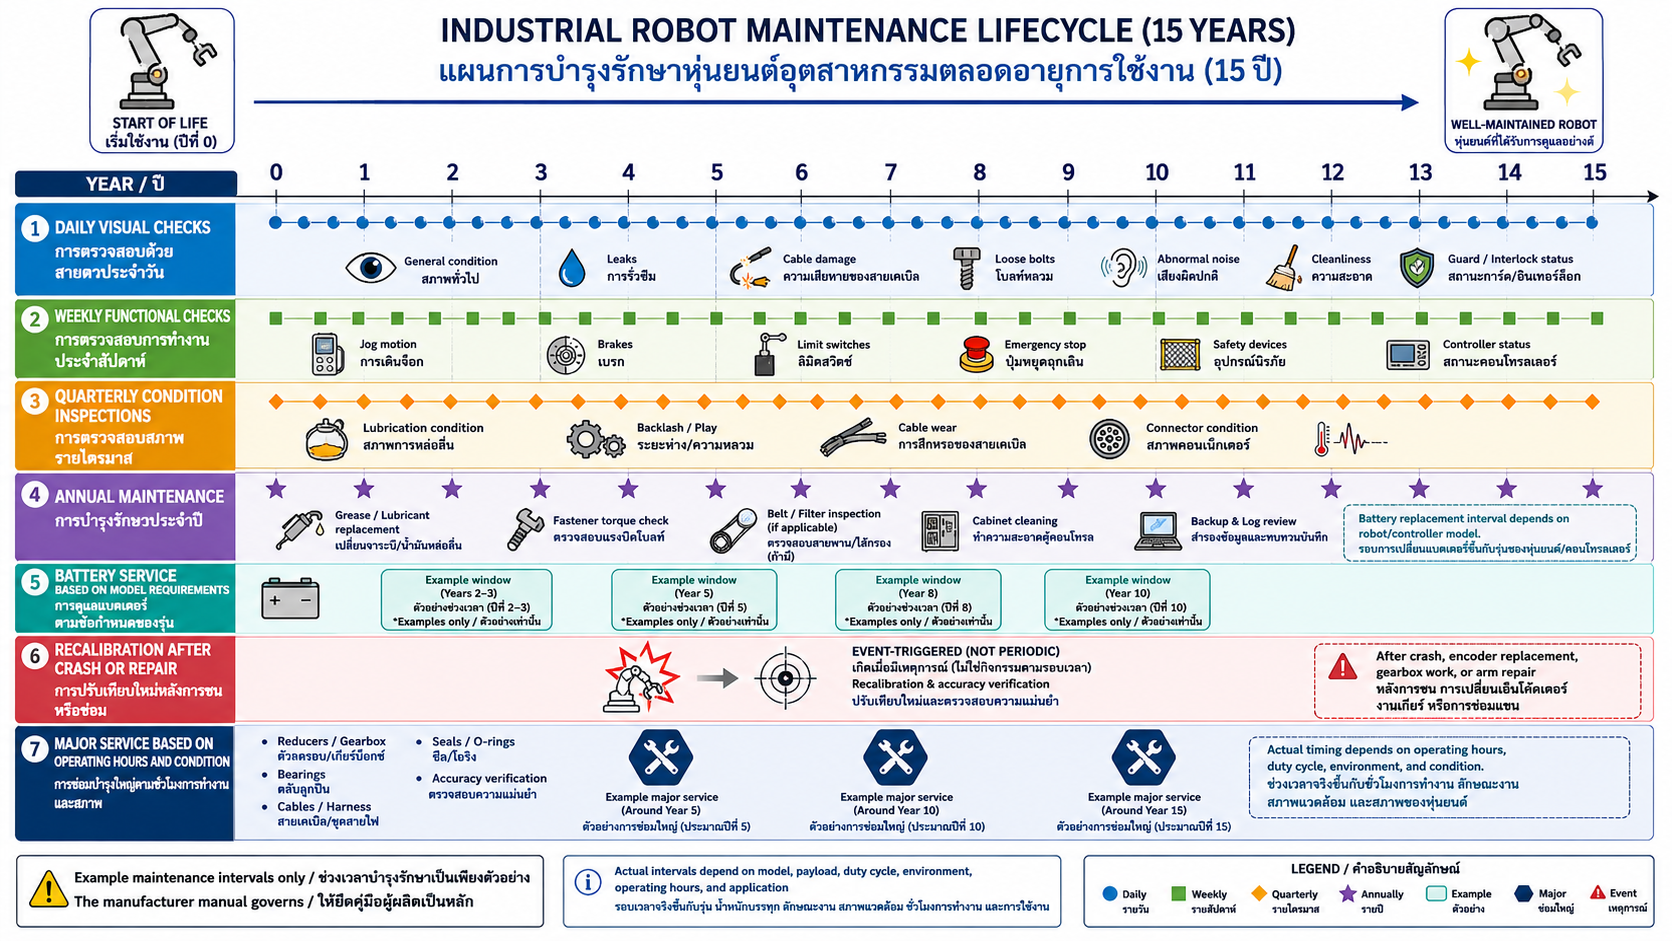
\includegraphics[width=0.8\textwidth]{images/chapter8/figure-04.png}
    \caption{แผน PM ตลอดวงจรชีวิตหุ่นยนต์}
\end{figure}

% [รูปที่ 8.5: Mastering Marks และการตั้งตำแหน่งอ้างอิง]
% ประเภทภาพ: Technical Illustration
% ตำแหน่งที่แนะนำ: หลังหัวข้อ 7.5.7
% วัตถุประสงค์การเรียนรู้: แสดงหลักการจัดแนว Mark ของ Joint ก่อนทำ Mastering
% คำอธิบายภาพ: ภาพระยะใกล้ของ Joint หุ่นยนต์ที่มี Witness Marks สองด้าน พร้อมลูกศรแสดงการจัดแนวและป้ายเตือนให้ใช้วิธีของผู้ผลิต
% องค์ประกอบที่ต้องมี: Joint housing, two alignment marks, axis direction, calibration tool placeholder, caution label
% ข้อความหรือป้ายกำกับ: Mastering Mark, Align per Product Manual, Do Not Estimate
% ภาษาของป้ายกำกับ: ไทยและอังกฤษ
% สัดส่วนภาพ: 16:9
% Image Generation Prompt: Close-up engineering textbook illustration of an industrial robot joint showing two mastering witness marks that must be aligned. Include axis direction arrow, a generic calibration tool reference, and a clear caution that the exact mastering procedure is model-specific and must follow the product manual. White background, realistic technical vector style, bilingual Thai-English labels, 16:9.
% Alt Text: รอย Mastering สองตำแหน่งบน Joint ที่ต้องจัดแนวตามคู่มือผู้ผลิต

\begin{figure}[htbp]
    \centering
    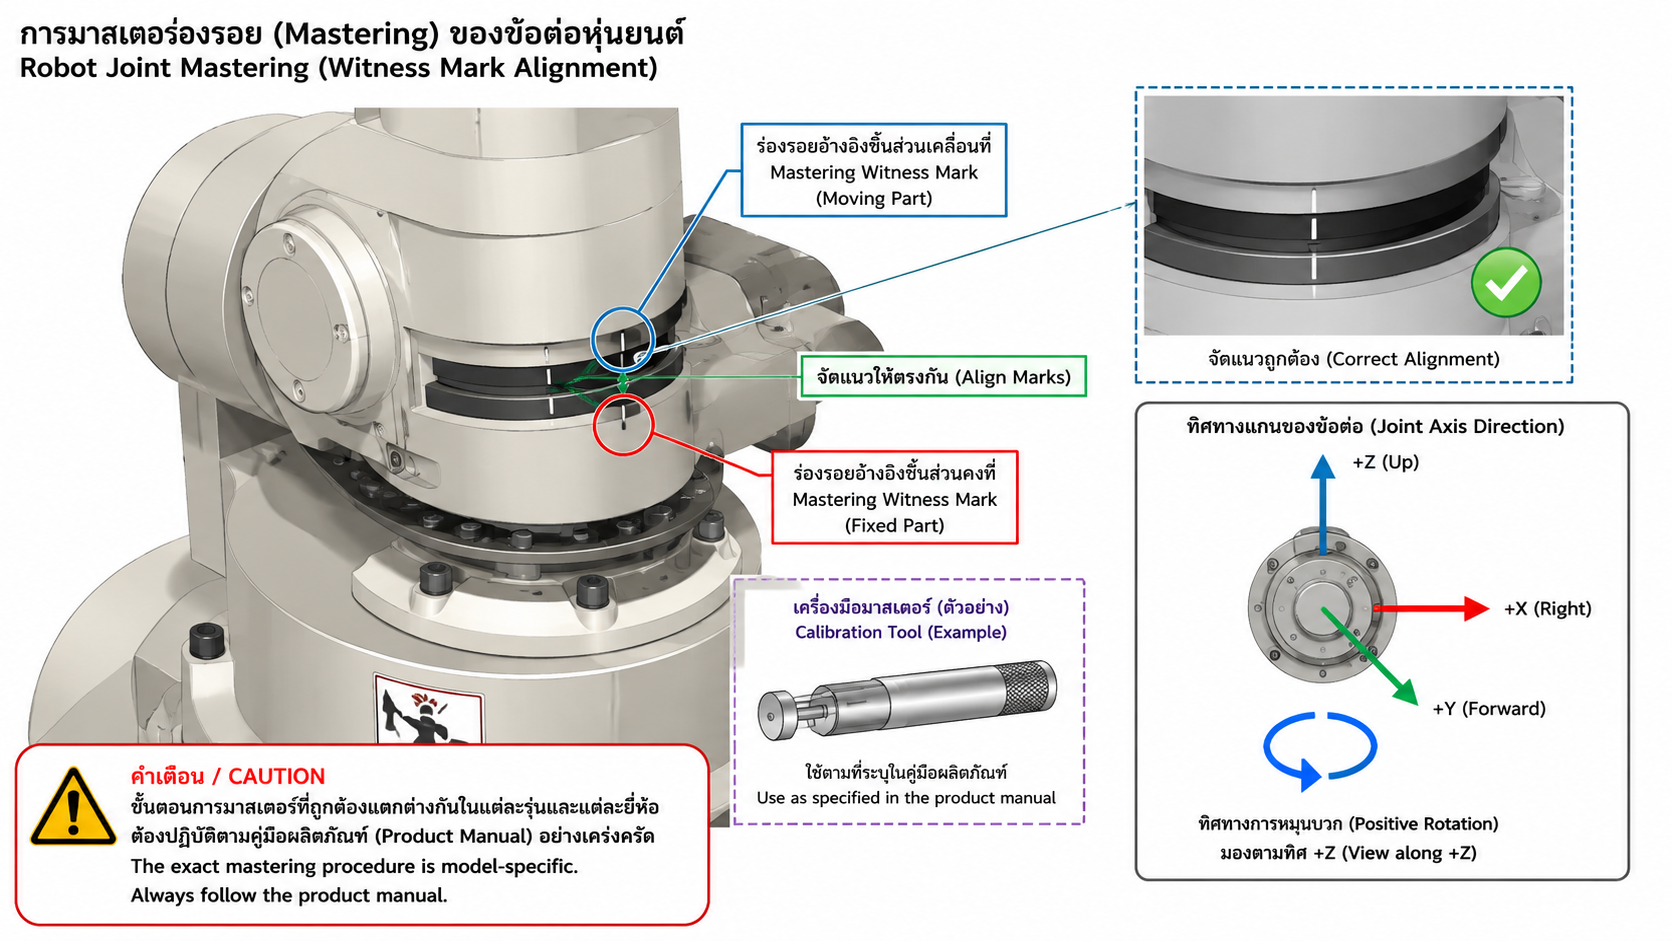
\includegraphics[width=0.8\textwidth]{images/chapter8/figure-05.png}
    \caption{Mastering Marks และการตั้งตำแหน่งอ้างอิง}
\end{figure}

\par\noindent\rule{\textwidth}{0.4pt}\par

\subsection{7.6 การแก้ไขปัญหาเบื้องต้น}

\subsubsection{7.6.1 หลักการ Troubleshooting}

Troubleshooting ที่มีประสิทธิภาพต้องแยก “อาการ” ออกจาก “สาเหตุ” ตัวอย่างเช่น หุ่นยนต์หยุดที่จุด Pick เป็นอาการ สาเหตุอาจเป็น Sensor ไม่มา Air Pressure ต่ำ โปรแกรมรอสัญญาณผิด Address Gripper จับไม่สำเร็จ หรือ Safety Stop จากอุปกรณ์อื่น การเปลี่ยน Parameter โดยยังไม่ระบุสาเหตุอาจทำให้ปัญหาซับซ้อนและสร้างความเสี่ยง

กระบวนการพื้นฐาน 6 ขั้น

\begin{enumerate}
    \item \textbf{สังเกตอาการ} — เกิดเมื่อใด จุดใด เกิดซ้ำหรือไม่ และเกิดหลังการเปลี่ยนแปลงใด
    \item \textbf{อ่านข้อมูลระบบ} — Alarm Code, Event Log, Program Line, I/O State และ Axis Data
    \item \textbf{ทำให้ระบบปลอดภัย} — หยุด Cycle แยกพลังงานเมื่อจำเป็น และห้าม Reset ซ้ำโดยไม่เข้าใจเงื่อนไข
    \item \textbf{สร้างสมมติฐาน} — จัดลำดับสาเหตุจากเป็นไปได้สูงและตรวจง่ายไปต่ำ
    \item \textbf{ทดสอบทีละส่วน} — เปลี่ยนตัวแปรครั้งละหนึ่งอย่างและบันทึกผล
    \item \textbf{ยืนยันและป้องกันซ้ำ} — ทดสอบหลาย Cycle คืนค่า Guard/Parameter บันทึก Root Cause และ Action
\end{enumerate}

\subsubsection{7.6.2 การจำแนกปัญหา}

\begin{table}[htbp]
    \centering
    \small
    \begin{tabularx}{\textwidth}{@{}L{0.20\textwidth}L{0.30\textwidth}Y@{}}
        \hline
        \textbf{กลุ่มปัญหา} & \textbf{ตัวอย่างอาการ} & \textbf{ข้อมูลที่ควรตรวจ} \\
        \hline
        Safety & Protective Stop, Gate Open, Chain Fault & Safety PLC, Gate Switch, E-stop, Scanner Zone, Reset Sequence \\
        Servo/Drive & Overcurrent, Overload, Overtemperature & Payload, Collision, Brake, Cable, Axis Load, Speed/Acceleration \\
        Position Feedback & Encoder Alarm, Position Lost & Encoder Cable, Battery, Connector, Mastering Status \\
        Mechanical & เสียง สั่น Backlash รั่ว & Gearbox, Bearing, Fastener, Tool, Dress Pack \\
        I/O/Peripheral & Wait ค้าง Gripper ไม่ตอบ & Input State, Output Voltage, Air/Vacuum, Sensor Alignment \\
        Program/Logic & Jump ผิด Loop ไม่จบ & Program Pointer, Register, Label, Timeout, Recipe \\
        Communication & PLC/Fieldbus Disconnect & Network Status, Node, Cable, Address, Watchdog \\
        Process & Weld Fault, Pick Fail, Quality Drift & Process Parameter, Consumable, Tool Wear, Part Tolerance \\
        \hline
    \end{tabularx}
\end{table}

\subsubsection{7.6.3 การอ่าน Alarm อย่างเป็นระบบ}

เมื่อพบ Alarm ควรบันทึก

\begin{itemize}
    \item วันและเวลา
    \item รหัสและข้อความเต็ม
    \item Program และ Line ที่เกิด
    \item Operating Mode
    \item ตำแหน่ง Joint/TCP
    \item I/O และ State ของอุปกรณ์
    \item Payload/Recipe ที่ใช้งาน
    \item การเปลี่ยนแปลงก่อนเกิด Alarm
    \item การดำเนินการที่ทำและผลลัพธ์
\end{itemize}

การ Reset Alarm โดยไม่บันทึกข้อมูลทำให้สูญเสียหลักฐานสำคัญและอาจทำให้ความผิดปกติเกิดซ้ำ

\subsubsection{ตาราง 8.6 ตัวอย่าง Alarm Code ตามขอบเขตที่กำหนด}

\begin{table}[htbp]
    \centering
    \small
    \begin{tabularx}{\textwidth}{@{}L{0.16\textwidth}L{0.28\textwidth}Y@{}}
        \hline
        \textbf{Error Code} & \textbf{ความหมายที่ใช้ในตัวอย่าง} & \textbf{แนวทางตรวจสอบเบื้องต้น} \\
        \hline
        SRVO-003 & Encoder Disconnect & ทำให้ระบบปลอดภัย ตรวจ Connector และสาย Feedback ตามคู่มือ \\
        SRVO-006 & Overcurrent & ตรวจการชน โหลด Brake สายมอเตอร์ และค่าความเร่ง ห้าม Reset ซ้ำต่อเนื่อง \\
        SRVO-012 & Overload & ตรวจ Payload, Center of Gravity, Duty Cycle และกลไกติดขัด \\
        SRVO-062 & Pulse/Position-related mismatch ตามตัวอย่าง & ตรวจข้อความ Alarm ฉบับเต็ม Battery และ Mastering Status ก่อนทำ Mastering \\
        SRVO-064 & Over-speed-related alarm ตามตัวอย่าง & ตรวจคำสั่ง Speed, Parameter, Feedback และสภาพกลไกตาม Manual \\
        SRVO-230 & Safety chain-related fault ตามตัวอย่าง & ตรวจ Safety Chain, Gate, E-stop และ Safety Hardware โดยผู้มีความสามารถ \\
        \hline
    \end{tabularx}
\end{table}

\begin{quote}
\textbf{ข้อจำกัดของตาราง:} รหัส Alarm และความหมายอาจแตกต่างตาม Controller Family, Software Option และ Revision ตารางนี้คงรายการตามขอบเขตบทเพื่อการฝึกวิเคราะห์เท่านั้น ก่อนปฏิบัติจริงต้องเปิด Alarm Code Manual ของ Controller และใช้ข้อความ Alarm เต็มจากหน้าจอเป็นแหล่งอ้างอิงหลัก
\end{quote}

\subsubsection{7.6.4 Fault Isolation}

การแยกสาเหตุควรเริ่มจากหลักฐาน ไม่ใช่การเปลี่ยนอะไหล่โดยคาดเดา ตัวอย่างกรณี Gripper ไม่ยืนยัน

\begin{verbatim}
อาการ: WAIT GRIP_OK ค้าง
    |-- Output GRIP_CLOSE ไม่ ON -> ตรวจ Program/Interlock/Output Module
    |-- Output ON แต่ Solenoid ไม่ทำงาน -> ตรวจแรงดัน สาย วาล์ว
    |-- Solenoid ทำงานแต่ Gripper ไม่ขยับ -> ตรวจ Air Pressure/กลไกติดขัด
    |-- Gripper ขยับแต่ Sensor ไม่ ON -> ตรวจตำแหน่ง Sensor/สาย/Input
    `-- Input ON ที่ Module แต่ Robot ไม่เห็น -> ตรวจ Mapping/Fieldbus
\end{verbatim}

การไล่ตามลำดับดังกล่าวลดการถอดอุปกรณ์โดยไม่จำเป็นและทำให้รายงาน Root Cause ชัดเจน

\subsubsection{7.6.5 Safe Recovery}

หลังแก้สาเหตุ ต้องวางแผน Recovery ตาม State ของระบบ

\begin{enumerate}
    \item ยืนยันว่าบุคลากรออกจากพื้นที่อันตราย
    \item คืน Guard, Connector และ Safety Device ครบ
    \item ตรวจว่าหุ่นยนต์ถือชิ้นงานหรือไม่
    \item ตรวจว่า Clamp, Machine Door, Conveyor และ Tool อยู่สถานะใด
    \item เลือก Recovery Routine หรือ Jog ไปยัง Safe Pose ที่กำหนด
    \item หลีกเลี่ยงการ Jump ข้ามคำสั่งที่ทำให้ I/O ไม่สอดคล้องกับสภาพจริง
    \item Reset Counter/State เฉพาะค่าที่จำเป็น
    \item Dry Run หนึ่ง Cycle ที่ความเร็วต่ำ
    \item จึงคืน Automatic Mode ตามขั้นตอนอนุมัติ
\end{enumerate}

% [รูปที่ 8.6: Flowchart การ Troubleshooting หุ่นยนต์]
% ประเภทภาพ: Flowchart
% ตำแหน่งที่แนะนำ: หลังหัวข้อ 7.6.1
% วัตถุประสงค์การเรียนรู้: แสดงลำดับสังเกต–ทำให้ปลอดภัย–วิเคราะห์–ทดสอบ–ยืนยัน
% คำอธิบายภาพ: เริ่มจาก Symptoms ไป Alarm/Log จากนั้น Safe State, Hypothesis, Test One Variable, Verify, Document และ Decision Loop กลับเมื่อยังไม่พบสาเหตุ
% องค์ประกอบที่ต้องมี: Start, Symptoms, Safety, Data Collection, Hypothesis, Test, Result, Verify, Record, Escalate
% ข้อความหรือป้ายกำกับ: Do not bypass safety, Change one variable at a time
% ภาษาของป้ายกำกับ: ไทยและอังกฤษ
% สัดส่วนภาพ: 16:9
% Image Generation Prompt: Systematic industrial robot troubleshooting flowchart: observe symptoms, read alarm and event logs, place system in a safe state, collect hardware and software evidence, form hypotheses, test one variable at a time, verify the repair, document root cause, and escalate when unresolved. Include decision loops and a warning not to bypass safety. Clean engineering textbook vector style, bilingual Thai-English labels, white background, 16:9.
% Alt Text: ผังงานการแก้ปัญหาจากอาการไปสู่การยืนยันและบันทึกสาเหตุ

\begin{figure}[htbp]
    \centering
    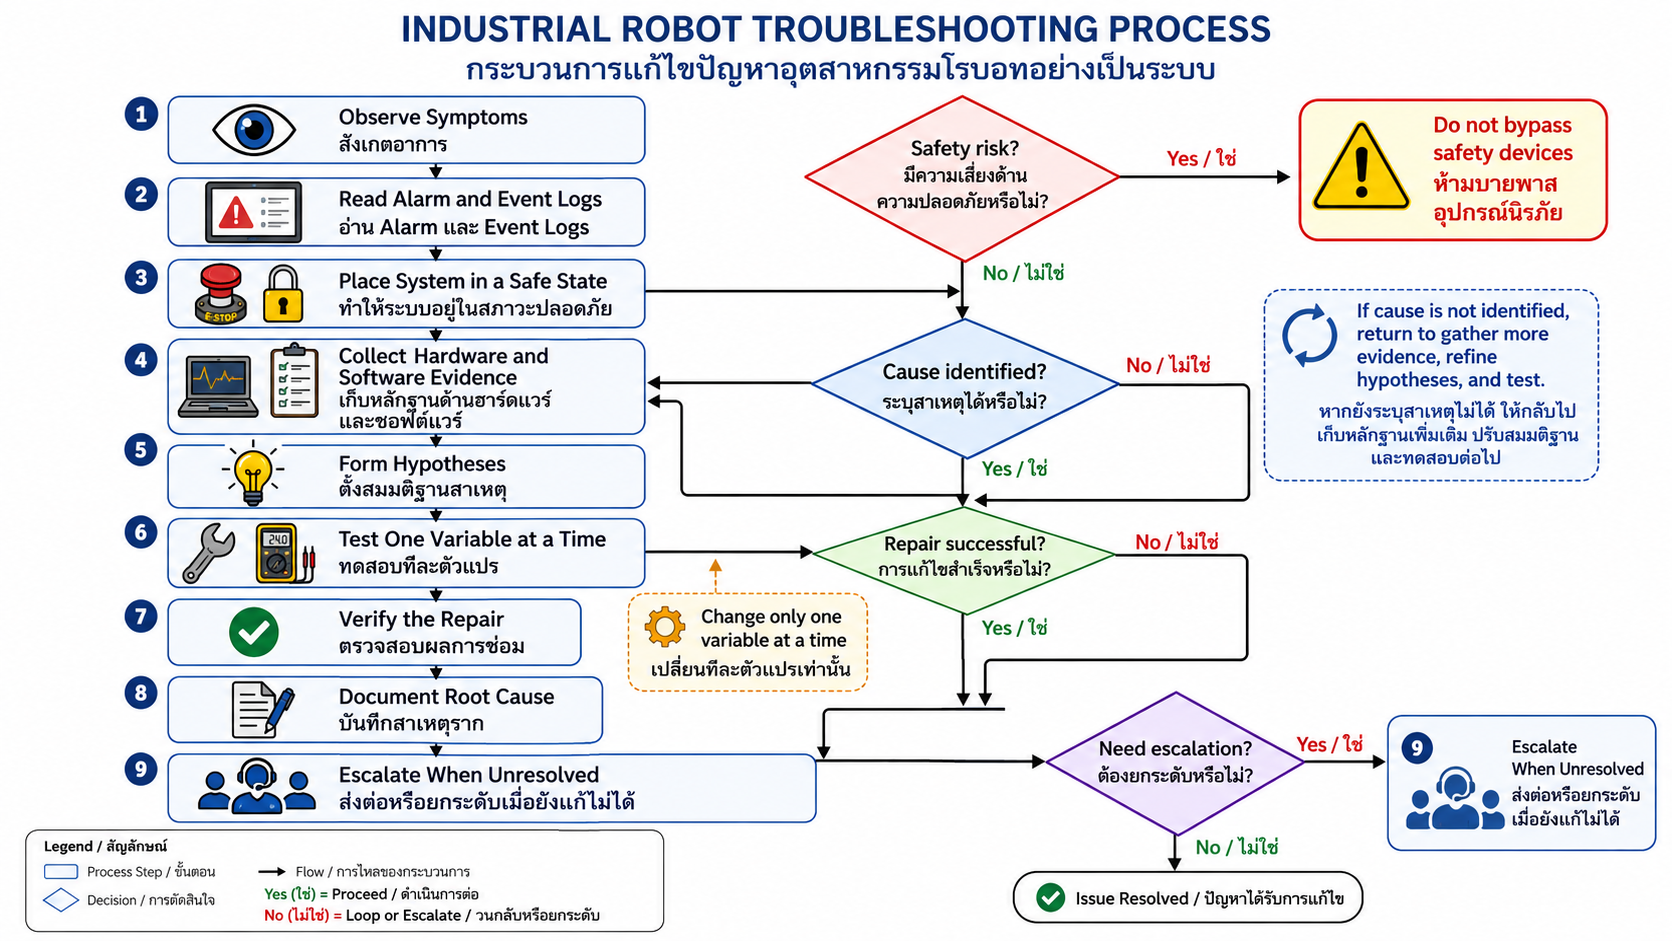
\includegraphics[width=0.8\textwidth]{images/chapter8/figure-06.png}
    \caption{Flowchart การ Troubleshooting หุ่นยนต์}
\end{figure}

\par\noindent\rule{\textwidth}{0.4pt}\par

\subsection{7.7 ความปลอดภัยในการทำงานกับหุ่นยนต์}

\subsubsection{7.7.1 กรอบมาตรฐานที่เกี่ยวข้อง}

การจัดการความปลอดภัยของหุ่นยนต์อุตสาหกรรมต้องพิจารณาทั้งตัวหุ่นยนต์และการรวมเป็นเซลล์

\begin{itemize}
    \item \textbf{ISO 10218-1:2025} ครอบคลุมข้อกำหนดด้านการออกแบบและการลดความเสี่ยงของ Industrial Robot
    \item \textbf{ISO 10218-2:2025} ครอบคลุม Robot Application, Integration, Commissioning, Operation และ Maintenance ของ Robot Cell
    \item \textbf{ISO 12100:2010} ให้หลัก Risk Assessment และ Risk Reduction ของเครื่องจักร
    \item \textbf{ISO 13855:2024} ใช้พิจารณาตำแหน่งและมิติของ Safeguard ตามการเข้าถึงของร่างกาย
    \item \textbf{ISO 13849-1:2023} ให้หลักการออกแบบ Safety-related Parts of Control Systems และ Performance Level
    \item \textbf{ISO 11161:2007/Amd 1:2010} ยังเป็นมาตรฐานปัจจุบันสำหรับ Integrated Manufacturing Systems ณ วันที่จัดทำเอกสาร แต่มีฉบับใหม่อยู่ระหว่างกระบวนการแทนที่
    \item \textbf{ข้อกำหนด LOTO ของสถานประกอบการและกฎหมายที่ใช้บังคับ} ต้องนำมาใช้กับงานซ่อมบำรุงและการควบคุมพลังงานอันตราย
\end{itemize}

การกล่าวว่า Safety PLC เป็น “SIL 2–3 หรือ PL d–e” โดยไม่ทำ Risk Assessment และ Validation ไม่เพียงพอ ระดับที่ต้องการต้องได้จากการประเมินความเสี่ยงและการออกแบบ Safety Function แต่ละฟังก์ชัน

\subsubsection{7.7.2 ลำดับชั้นการลดความเสี่ยง}

แนวทางตาม ISO 12100 เริ่มจาก

\begin{enumerate}
    \item \textbf{Inherently Safe Design:} ลดอันตรายด้วยการออกแบบ เช่น ลดขอบคม ลดแรง/ความเร็ว หรือจำกัดช่วงเคลื่อนที่
    \item \textbf{Safeguarding and Protective Measures:} รั้ว Interlock, Light Curtain, Scanner, Pressure Mat และ Safety Function
    \item \textbf{Information for Use:} Warning, Procedure, Training, PPE และ Sign
\end{enumerate}

PPE และป้ายเตือนไม่สามารถทดแทน Guard หรือการแยกพลังงานเมื่อยังมีอันตรายจากการเคลื่อนที่ของหุ่นยนต์

\subsubsection{7.7.3 Operating Modes และการสอน}

ระบบหุ่นยนต์อาจมี Automatic, Manual Reduced-speed และโหมดอื่นตามผู้ผลิต ในห้องปฏิบัติการควรกำหนดว่า

\begin{itemize}
    \item การสอนและ Touch-up ใช้ Manual Reduced-speed เท่านั้น
    \item ใช้ Enabling Device ตามการออกแบบของ Teach Pendant
    \item มีผู้ควบคุม Pendant คนเดียวและมีอำนาจหยุดการทดลอง
    \item ห้ามผู้เรียนอยู่ในพื้นที่พร้อมกันหลายคนโดยไม่มีบทบาทชัดเจน
    \item ห้ามใช้ Automatic เมื่อประตูเปิดหรือ Safeguard ถูก Bypass
    \item ค่า 250 mm/s มักพบเป็นขีดจำกัดอ้างอิงสำหรับการเคลื่อนที่แบบ Manual Reduced-speed ในระบบอุตสาหกรรมหลายชนิด แต่ต้องใช้ค่าที่มาตรฐานและผู้ผลิตกำหนดสำหรับระบบจริง ไม่ควรตั้งค่าโดยอาศัยตัวเลขนี้เพียงอย่างเดียว
\end{itemize}

\subsubsection{7.7.4 Safety Distance}

รูปแบบสมการพื้นฐานที่ใช้ในบทเรียนคือ

\[
S=K\times T+C
\]

เมื่อ

\begin{itemize}
    \item $S$ คือระยะต่ำสุดจาก Detection Zone ถึง Hazard Zone หน่วย mm
    \item $K$ คือความเร็วเข้าหาที่มาตรฐานกำหนด หน่วย mm/s
    \item $T$ คือ \textbf{เวลาตอบสนองรวมของระบบ} หน่วย s
    \item $C$ คือระยะเพิ่มที่สัมพันธ์กับการเข้าถึงหรือการทะลุผ่านอุปกรณ์ตรวจจับ หน่วย mm
\end{itemize}

เวลารวม $T$ ต้องรวมองค์ประกอบที่เกี่ยวข้อง เช่น

\[
T=T_{sensor}+T_{logic}+T_{network}+T_{machine\ stop}+T_{margin}
\]

การใช้เฉพาะ Response Time ของ Light Curtain โดยไม่รวมเวลาหยุดของหุ่นยนต์จะทำให้ระยะที่คำนวณต่ำเกินจริง

\subsubsection{ตัวอย่างที่ 8.5 การคำนวณระยะป้องกันตามข้อมูลโจทย์}

\textbf{ตัวอย่างเพิ่มเติมเพื่อการเรียนรู้}

กำหนด $K=2{,}000$ mm/s, $T=15$ ms และ $C=850$ mm โดยสมมติว่า 15 ms เป็นเวลารวมทั้งหมดตามโจทย์

แปลงหน่วย

\[
T=15\text{ ms}=0.015\text{ s}
\]

คำนวณ

\[
S=(2{,}000)(0.015)+850=30+850=880\text{ mm}
\]

ดังนั้นระยะต่ำสุดตามสมมติฐานของโจทย์คือ \textbf{880 mm}

\textbf{ข้อควรระวังในการออกแบบจริง:} หาก 15 ms เป็นเพียงเวลาของ Sensor ต้องวัดหรือใช้ค่า Stop Time รวมของ Robot Cell แล้วคำนวณใหม่ รวมทั้งตรวจสูตรและค่าคงที่สำหรับชนิดอุปกรณ์ตาม ISO 13855:2024 และคู่มือผู้ผลิต

\subsubsection{7.7.5 Warning Zone และ Protective Zone}

Area Scanner สามารถกำหนดหลาย Zone เช่น

\begin{itemize}
    \item \textbf{Warning Zone:} ตรวจพบบุคคลแล้วเตือน ลดความเร็ว หรือเตรียมหยุดตามการออกแบบ
    \item \textbf{Protective Zone:} การบุกรุกทำให้เกิด Protective Stop ที่ผ่านการออกแบบและ Validation
    \item \textbf{Restart Interlock:} ระบบต้องไม่เริ่มใหม่โดยอัตโนมัติเมื่อพื้นที่กลับมาว่าง หากยังมีความเป็นไปได้ว่าบุคคลอยู่ในพื้นที่อันตรายหรือเงื่อนไข Reset ไม่ครบ
\end{itemize}

การกำหนด Zone ต้องพิจารณา Stop Time, Scanner Resolution, Field Tolerance, Floor Reflection, Blind Spot, Tool Extension และตำแหน่งทุกแกน ไม่ใช่ดูเฉพาะฐานหุ่นยนต์

\subsubsection{7.7.6 LOTO สำหรับงานบำรุงรักษา}

ขั้นตอนทั่วไปของ LOTO

\begin{enumerate}
    \item แจ้งผู้เกี่ยวข้องและระบุขอบเขตงาน
    \item หยุดระบบด้วยวิธีปกติ
    \item ระบุแหล่งพลังงานทั้งหมด เช่น ไฟฟ้า Pneumatic, Hydraulic, Gravity, Spring และ Stored Energy
    \item แยกแหล่งพลังงานด้วย Disconnect/Valve ที่เหมาะสม
    \item ล็อกและติดป้ายโดยผู้ปฏิบัติงานแต่ละคน
    \item ระบายหรือควบคุม Stored Energy
    \item ยืนยัน Zero-energy State ตามวิธีที่กำหนด
    \item ดำเนินงาน
    \item ตรวจพื้นที่และประกอบ Guard/Connector กลับ
    \item นำ Lock ออกโดยผู้เป็นเจ้าของตาม Procedure
    \item แจ้งผู้เกี่ยวข้องและคืนระบบอย่างควบคุม
\end{enumerate}

การกด Hold, Cycle Stop หรือ Emergency Stop \textbf{ไม่เท่ากับ LOTO} เพราะพลังงานยังอาจคงอยู่และระบบอาจถูก Reset ได้

\subsubsection{7.7.7 ขั้นตอนก่อนเข้าสู่พื้นที่ Safeguarded Space}

\begin{verbatim}
1. หยุด Cycle ตามขั้นตอนที่อนุมัติ
2. ยืนยันสถานะหุ่นยนต์และอุปกรณ์รอบข้าง
3. เปิด Gate ผ่าน Interlock โดยไม่ Bypass
4. หากเป็นงานซ่อม/ปรับแต่งที่สัมผัสอันตราย ให้ทำ LOTO
5. หากเป็นงาน Teaching ที่ได้รับอนุญาต ใช้ Manual Reduced-speed และ Enabling Device
6. นำ Teach Pendant เข้าไปกับผู้ควบคุม ห้ามวางไว้นอกพื้นที่ให้ผู้อื่นสั่ง
7. ตรวจ Escape Path และ Pinch/Crush Zone
8. สื่อสารบทบาทของทุกคนก่อนเริ่มเคลื่อนที่
\end{verbatim}

% [รูปที่ 8.7: Warning Zone และ Protective Zone ของเซลล์หุ่นยนต์]
% ประเภทภาพ: Safety Zone Diagram
% ตำแหน่งที่แนะนำ: หลังหัวข้อ 7.7.5
% วัตถุประสงค์การเรียนรู้: แสดงความสัมพันธ์ของ Hazard Zone, Protective Zone, Warning Zone, Scanner และ Gate
% คำอธิบายภาพ: มุมมองด้านบนของเซลล์หุ่นยนต์ มีรั้ว ประตู Interlock Scanner Field สองระดับ และลูกศรระยะหยุด
% องค์ประกอบที่ต้องมี: Robot, swept area, fence, gate, light curtain or scanner, warning field, protective field, reset station outside zone
% ข้อความหรือป้ายกำกับ: Hazard Zone, Protective Zone, Warning Zone, Interlocked Gate, Manual Reset
% ภาษาของป้ายกำกับ: ไทยและอังกฤษ
% สัดส่วนภาพ: 16:9
% Image Generation Prompt: Top-view industrial robot cell safety diagram with a six-axis robot, swept hazard area, perimeter fence, interlocked gate, safety laser scanner, outer warning zone, inner protective zone, and a manual reset station located outside the safeguarded space with clear visibility. Show separation distance and stopping direction arrows. Clean engineering vector style, bilingual Thai-English labels, white background, 16:9.
% Alt Text: มุมมองด้านบนของเซลล์หุ่นยนต์ที่มีเขตเตือน เขตป้องกัน รั้ว ประตู และจุด Reset นอกพื้นที่

\begin{figure}[htbp]
    \centering
    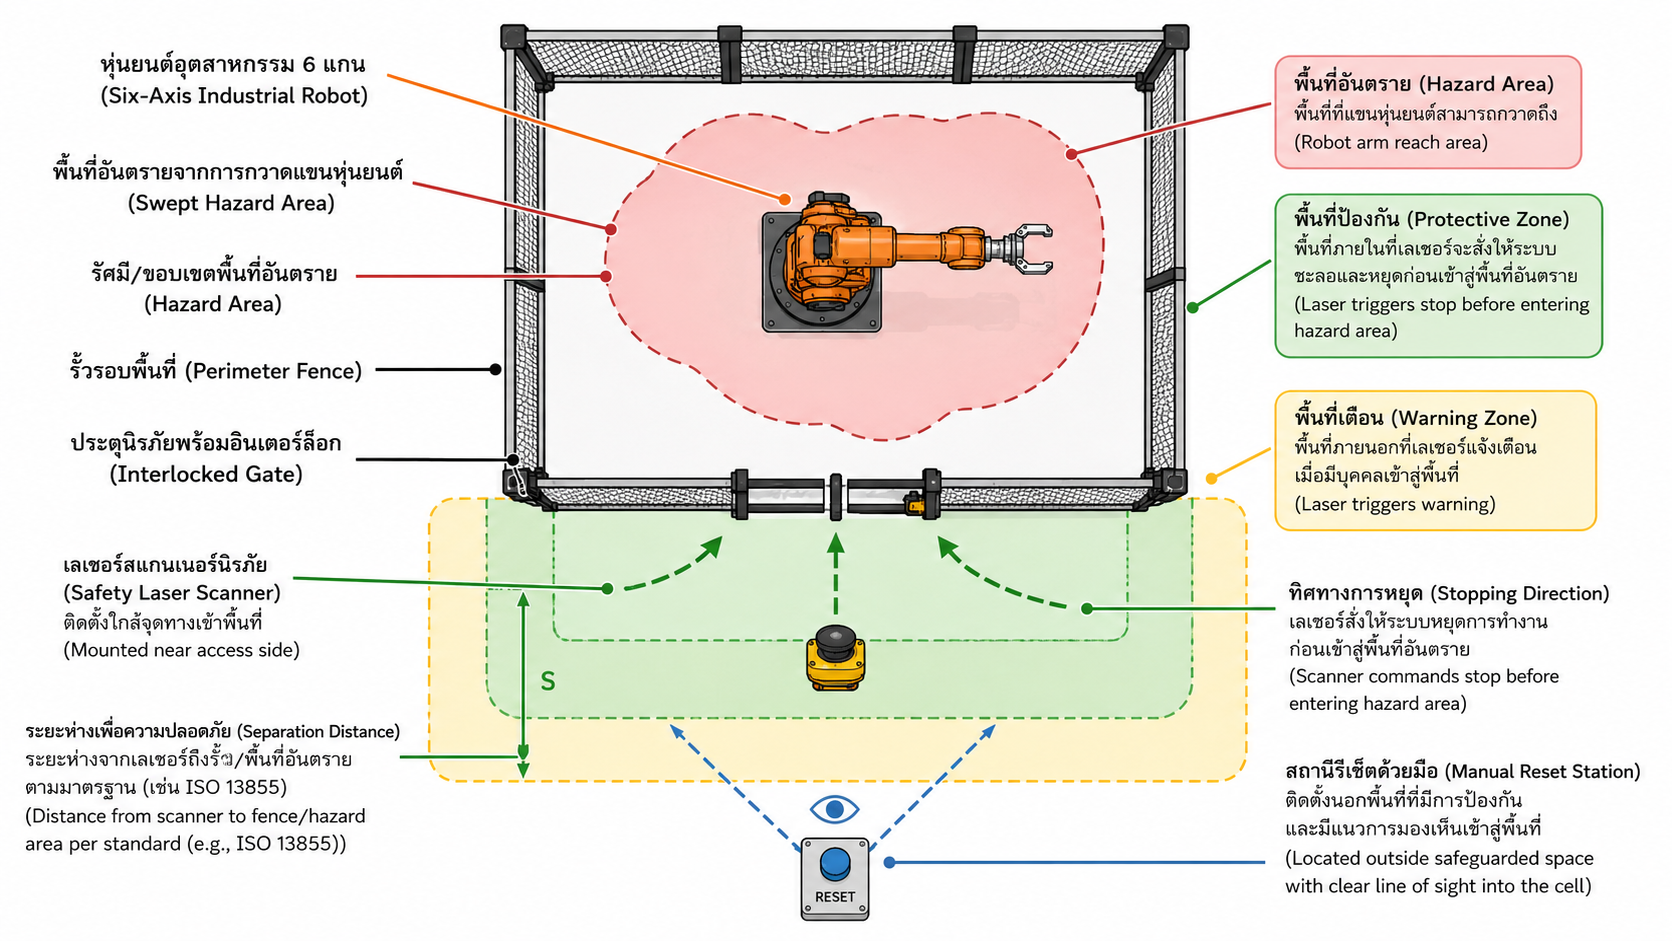
\includegraphics[width=0.8\textwidth]{images/chapter8/figure-07.png}
    \caption{Warning Zone และ Protective Zone ของเซลล์หุ่นยนต์}
\end{figure}

\par\noindent\rule{\textwidth}{0.4pt}\par

\subsection{7.8 เปรียบเทียบภาษาโปรแกรมและซอฟต์แวร์จากผู้ผลิต}

\subsubsection{ตาราง 8.7 ภาษาโปรแกรมหุ่นยนต์จากผู้ผลิตชั้นนำ}

\begin{table}[htbp]
    \centering
    \small
    \begin{tabularx}{\textwidth}{@{}L{0.13\textwidth}L{0.22\textwidth}L{0.17\textwidth}L{0.18\textwidth}Y@{}}
        \hline
        \textbf{ผู้ผลิต} & \textbf{ภาษา/สภาพแวดล้อม} & \textbf{Extension ตัวอย่าง} & \textbf{คำสั่งเคลื่อนที่หลัก} & \textbf{ซอฟต์แวร์ Offline/Simulation} \\
        \hline
        FANUC & TP Language / KAREL & \texttt{.LS}, \texttt{.TP}, \texttt{.KL} & \texttt{J}, \texttt{L}, \texttt{C} & ROBOGUIDE \\
        ABB & RAPID & \texttt{.MOD} & \texttt{MoveJ}, \texttt{MoveL}, \texttt{MoveC} & RobotStudio \\
        KUKA & KRL & \texttt{.SRC}, \texttt{.DAT} & \texttt{PTP}, \texttt{LIN}, \texttt{CIRC} & KUKA.Sim หรือแพลตฟอร์มวิศวกรรมที่รองรับรุ่นนั้น \\
        Yaskawa & INFORM & \texttt{.JBI} & \texttt{MOVJ}, \texttt{MOVL}, \texttt{MOVC} & MotoSim EG-VRC \\
        Mitsubishi & MELFA-BASIC & \texttt{.MB5} หรือรูปแบบตาม Controller & \texttt{MOV}, \texttt{MVS}, \texttt{MVR} & RT ToolBox3 \\
        Universal Robots & PolyScope / URScript & \texttt{.URP}, \texttt{.script} & \texttt{movej}, \texttt{movel}, \texttt{movec} & URSim/PolyScope Simulation \\
        \hline
    \end{tabularx}
\end{table}

ตารางนี้ใช้เพื่อเปรียบเทียบแนวคิด ไม่ควรสรุปว่าคำสั่งต่างยี่ห้อมีพฤติกรรมเหมือนกันทุกประการ ความหมายของ Speed, Zone, Orientation Interpolation, Configuration และ Error Handling ต่างกันตามระบบ

\subsubsection{ตาราง 8.8 แนวคิดที่เทียบเคียงข้ามผู้ผลิต}

\begin{table}[htbp]
    \centering
    \small
    \begin{tabularx}{\textwidth}{@{}L{0.22\textwidth}L{0.14\textwidth}L{0.17\textwidth}L{0.22\textwidth}Y@{}}
        \hline
        \textbf{แนวคิด} & \textbf{FANUC} & \textbf{ABB} & \textbf{KUKA} & \textbf{Universal Robots} \\
        \hline
        Joint Motion & \texttt{J} & \texttt{MoveJ} & \texttt{PTP} & \texttt{movej} \\
        Linear TCP Motion & \texttt{L} & \texttt{MoveL} & \texttt{LIN} & \texttt{movel} \\
        Circular TCP Motion & \texttt{C} & \texttt{MoveC} & \texttt{CIRC} & \texttt{movec} \\
        Exact Stop & \texttt{FINE} & \texttt{fine} & Approximation off/exact target & Blend radius \texttt{r=0} โดยแนวคิด \\
        Blending & \texttt{CNT} & \texttt{z10}, \texttt{z50}, ... & \texttt{\$APO}/Approximation & Blend radius \texttt{r} \\
        User Frame & \texttt{UFRAME} & \texttt{wobjdata} & Base & Feature/Plane \\
        Tool Frame & \texttt{UTOOL} & \texttt{tooldata} & Tool & TCP \\
        \hline
    \end{tabularx}
\end{table}

\par\noindent\rule{\textwidth}{0.4pt}\par

\subsection{7.9 กิจกรรมปฏิบัติการประจำบท}

\subsection{กิจกรรมปฏิบัติการที่ 8-1: การสอนตำแหน่งและเขียนโปรแกรม Pick-and-Place}

\subsubsection{1. วัตถุประสงค์}

เมื่อจบกิจกรรม นักศึกษาสามารถ

\begin{itemize}
    \item เลือก Joint, World, Tool และ User Coordinate ในการ Jog ได้เหมาะสม
    \item สอน Home, Approach, Pick, Place และ Retreat Point ได้
    \item เขียนโปรแกรม Motion, Gripper I/O, Wait และ Timeout ได้
    \item เปรียบเทียบผลของ Fine กับ Blending ต่อ Path และ Cycle Time ได้
    \item ปฏิบัติงานใน Manual Reduced-speed โดยใช้ Enabling Device ได้ถูกต้อง
\end{itemize}

\subsubsection{2. หลักการและทฤษฎีที่เกี่ยวข้อง}

กิจกรรมใช้หลัก Coordinate Frame, TCP, Approach–Process–Retreat, PTP/Linear Motion, Digital I/O และ Handshake โปรแกรมต้องแยกจุด Approach ออกจากจุด Pick/Place และต้องรอสัญญาณ Gripper Confirm ก่อนยกชิ้นงาน

\subsubsection{3. อุปกรณ์ เครื่องมือ และซอฟต์แวร์}

\begin{table}[htbp]
    \centering
    \begin{tabular}{l r l}
        \hline
        \textbf{รายการ} & \textbf{จำนวน} & \textbf{ข้อกำหนด} \\
        \hline
        ชุดหุ่นยนต์เพื่อการศึกษา & 1 ชุด/กลุ่ม & มี Teach Pendant, Guard และ Manual Mode \\
        Gripper ที่ติดตั้งและตรวจสอบแล้ว & 1 ชุด & ใช้แรง/แรงดันตามระบบฝึก \\
        ชิ้นงานจำลองน้ำหนักเบา & 3–5 ชิ้น & ไม่มีขอบคม แตกง่าย หรืออันตราย \\
        ถาด Pick และ Place & อย่างละ 1 & ยึดกับโต๊ะหรือ Fixture \\
        Checklist ความปลอดภัย & 1 ชุด/กลุ่ม & ใช้ก่อนเปิด Motion \\
        Stopwatch/Controller Cycle Timer & 1 & ใช้วัดเวลาเทียบ \\
        ซอฟต์แวร์จำลอง ถ้ามี & 1 License/กลุ่ม & ใช้ตรวจเส้นทางก่อนหุ่นยนต์จริง \\
        \hline
    \end{tabular}
\end{table}

\subsubsection{4. แผนภาพหรือชุดทดลอง}

\begin{verbatim}
Pick Tray -> P_PICK_APP -> P_PICK
                         |  Gripper Close + Confirm
P_PLACE_APP -> P_PLACE -> Place Tray
                         |  Gripper Open + Confirm
Return -> P_HOME
\end{verbatim}

\subsubsection{5. ข้อควรระวังด้านความปลอดภัย}

\begin{itemize}
    \item ผู้ควบคุม Teach Pendant มีเพียงคนเดียวต่อรอบ
    \item เริ่มจาก Simulation หรือ Robot ไม่มีชิ้นงาน
    \item ใช้ Manual Reduced-speed และ Step/Single Block
    \item ห้ามเข้า Automatic ขณะ Gate เปิด
    \item ห้ามจับแขนหรือ End Effector ของหุ่นยนต์อุตสาหกรรมทั่วไปด้วยมือ
    \item ห้าม Bypass Gripper Sensor หรือ Safety Interlock เพื่อให้กิจกรรมผ่าน
    \item หากมีการเคลื่อนที่ผิดทิศ ให้ปล่อย Enabling Device หรือใช้วิธีหยุดที่ได้รับการฝึกทันที
\end{itemize}

\subsubsection{6. ขั้นตอนการปฏิบัติ}

\begin{enumerate}
    \item ทำ Pre-job Briefing และตรวจ Checklist ความปลอดภัย
    \item เปิดระบบตาม Standard Operating Procedure ของห้องปฏิบัติการ
    \item เลือก Tool Frame และ User Frame ที่อาจารย์กำหนด
    \item ตรวจ TCP ด้วยจุดอ้างอิงโดยไม่ชนหรือกด Tool ลงบน Jig
    \item Jog ด้วย Joint Coordinate ไปยัง \texttt{P\_HOME}
    \item ใช้ World Coordinate ไปยังบริเวณเหนือ Pick Fixture
    \item ใช้ Tool/User Coordinate สอน \texttt{P\_PICK\_APP} และ \texttt{P\_PICK}
    \item สอน \texttt{P\_PLACE\_APP} และ \texttt{P\_PLACE}
    \item เขียนโปรแกรมเริ่มต้นโดยใช้ Fine ทุกจุด
    \item เพิ่ม Gripper Close/Open และ Wait Confirm พร้อม Timeout
    \item ตรวจโปรแกรมด้วย Static Review
    \item ทดสอบแบบ Step โดยไม่ใช้ชิ้นงาน
    \item ทดสอบด้วยชิ้นงานจำลองเมื่ออาจารย์อนุญาต
    \item วัด Cycle Time จำนวน 3 รอบ
    \item เปลี่ยนเฉพาะจุดผ่านกลางอากาศเป็น Blend ระดับต่ำหรือกลาง
    \item ทดสอบ Path และ Clearance อีกครั้ง
    \item วัด Cycle Time 3 รอบและเปรียบเทียบ
    \item Backup โปรแกรมและส่ง Point List
\end{enumerate}

\subsubsection{7. ตารางบันทึกผล}

\begin{table}[htbp]
    \centering
    \begin{tabular}{l l l r l l l}
        \hline
        \textbf{จุด} & \textbf{Coordinate ที่ใช้สอน} & \textbf{Motion} & \textbf{Speed} & \textbf{Fine/Blend} & \textbf{Tool/User No.} & \textbf{ผลการตรวจ Clearance} \\
        \hline
        HOME &  &  &  &  &  &  \\
        PICK\_APP &  &  &  &  &  &  \\
        PICK &  &  &  &  &  &  \\
        PLACE\_APP &  &  &  &  &  &  \\
        PLACE &  &  &  &  &  &  \\
        \hline
    \end{tabular}
\end{table}

\begin{table}[htbp]
    \centering
    \begin{tabular}{l r r r r l}
        \hline
        \textbf{การทดลอง} & \textbf{Cycle 1 (s)} & \textbf{Cycle 2 (s)} & \textbf{Cycle 3 (s)} & \textbf{ค่าเฉลี่ย (s)} & \textbf{หมายเหตุ} \\
        \hline
        Fine ทุกจุด &  &  &  &  &  \\
        Blend เฉพาะจุดผ่าน &  &  &  &  &  \\
        \hline
    \end{tabular}
\end{table}

\subsubsection{8. การคำนวณและวิเคราะห์ผล}

ค่าเฉลี่ย Cycle Time

\[
\bar{t}=\frac{t_1+t_2+t_3}{3}
\]

ร้อยละการลด Cycle Time

\[
\%\text{Reduction}=\frac{\bar{t}_{Fine}-\bar{t}_{Blend}}{\bar{t}_{Fine}}\times100
\]

นักศึกษาต้องอธิบายว่าการลดเวลามาจากจุดใด และ Path Deviation ที่เพิ่มขึ้นยังอยู่ใน Clearance ที่ยอมรับได้หรือไม่

\subsubsection{9. การเปรียบเทียบผลจริงกับทฤษฎีหรือแบบจำลอง}

หากใช้ OLP ให้เปรียบเทียบ Cycle Time และ Path จาก Simulation กับระบบจริง พร้อมอธิบายความต่างจาก Acceleration Limit, Controller Option, Payload, I/O Delay และ Gripper Response

\subsubsection{10. คำถามหลังการทดลอง}

\begin{enumerate}
    \item เหตุใดจุด Pick และ Place จึงควรใช้ Fine มากกว่าจุดผ่านกลางอากาศ
    \item หากเปลี่ยน User Frame แล้วไม่สอนจุดใหม่ จุดทั้งหมดควรเปลี่ยนอย่างไร
    \item หาก \texttt{GRIP\_OK} ไม่มา โปรแกรมควรหยุดที่ State ใด
    \item จุดใดควรใช้ Linear Motion และเหตุใด
    \item Blending ที่มากเกินไปอาจทำให้เกิดความเสี่ยงใด
\end{enumerate}

\subsubsection{11. เกณฑ์การประเมิน}

\begin{table}[htbp]
    \centering
    \begin{tabular}{l r}
        \hline
        \textbf{เกณฑ์} & \textbf{คะแนน} \\
        \hline
        ความปลอดภัยและการใช้ Teach Pendant & 25 \\
        ความถูกต้องของ Tool/User Frame และ Point & 20 \\
        โปรแกรม Motion, I/O, Timeout & 25 \\
        การวัดและวิเคราะห์ Cycle Time & 15 \\
        การตั้งชื่อ Comment และ Backup & 10 \\
        การตอบคำถามหลังทดลอง & 5 \\
        \textbf{รวม} & \textbf{100} \\
        \hline
    \end{tabular}
\end{table}

\par\noindent\rule{\textwidth}{0.4pt}\par

\subsection{กิจกรรมปฏิบัติการที่ 8-2: Daily Check และการจัดทำแผน Preventive Maintenance}

\subsubsection{1. วัตถุประสงค์}

\begin{itemize}
    \item ตรวจสภาพภายนอกของหุ่นยนต์และ End Effector ได้อย่างเป็นระบบ
    \item แยก Normal Condition, Observation และ Defect ได้
    \item จัดทำ PM Schedule ตาม Manual-based, Time-based และ Condition-based ได้
    \item บันทึกหลักฐานโดยไม่แต่งค่าที่ไม่ได้วัด
\end{itemize}

\subsubsection{2. หลักการและทฤษฎีที่เกี่ยวข้อง}

PM ใช้การตรวจซ้ำตามรอบและเกณฑ์ที่กำหนด การสังเกตต้องอ้างอิง Baseline หรือคู่มือ ไม่ควรสรุปสาเหตุจากลักษณะภายนอกเพียงอย่างเดียว

\subsubsection{3. อุปกรณ์ เครื่องมือ และซอฟต์แวร์}

\begin{table}[htbp]
    \centering
    \begin{tabular}{l r l}
        \hline
        \textbf{รายการ} & \textbf{จำนวน} & \textbf{ข้อกำหนด} \\
        \hline
        หุ่นยนต์ที่หยุดและจัดสภาพปลอดภัย & 1 ชุด & ไม่อนุญาต Motion ระหว่าง Visual Check \\
        ไฟฉายแรงดันต่ำ & 1 & ใช้ส่องตรวจ ไม่สอดมือเข้า Pinch Point \\
        กระจกตรวจ & 1 & ด้ามยาว ไม่มีขอบคม \\
        Torque Mark Reference & 1 ชุด & ใช้สังเกต ไม่ขันจริงหากไม่มีค่าคู่มือ \\
        แบบฟอร์ม Daily/PM Record & 1 ชุด/กลุ่ม & มีช่องผู้ตรวจและหลักฐาน \\
        กล้องถ่ายภาพของหน่วยงาน & 1 & ไม่ถ่ายข้อมูลลับหรือ Serial ตามนโยบาย \\
        Product Manual ของรุ่นฝึก & 1 & ใช้หาค่ารอบและข้อกำหนด \\
        \hline
    \end{tabular}
\end{table}

\subsubsection{4. แผนภาพหรือวงจร}

ใช้รูปที่ 8.4 และแผนผังตำแหน่งตรวจของหุ่นยนต์รุ่นที่ห้องปฏิบัติการใช้งาน

\subsubsection{5. ข้อควรระวังด้านความปลอดภัย}

\begin{itemize}
    \item หยุดระบบและใช้วิธีแยกพลังงานตามขอบเขตงาน
    \item ไม่เปิด Cover หรือถอด Connector ในกิจกรรมพื้นฐาน
    \item ไม่เติม Grease ไม่ขัน Bolt และไม่เปลี่ยน Battery หากไม่มีคู่มือ เครื่องมือ และผู้ควบคุมที่ได้รับอนุญาต
    \item ห้ามยืนใต้ Payload หรือส่วนที่อาจตกจากแรงโน้มถ่วง
    \item ไม่ใช้มือสัมผัสบริเวณที่สงสัยว่าร้อนหรือมีรอยรั่ว
\end{itemize}

\subsubsection{6. ขั้นตอนการปฏิบัติ}

\begin{enumerate}
    \item อ่าน Manual หัวข้อ Maintenance Schedule ของรุ่นฝึก
    \item ระบุจุดตรวจรอบ Robot Base, Arm, Wrist, Tool และ Dress Pack
    \item ตรวจรอยรั่ว รอยแตก รอยขูด การบิดสาย และ Fastener Mark
    \item ตรวจ End Effector, Air Hose, Sensor และ Fixture
    \item ตรวจ Fan/Filter หรือ Controller Cabinet เฉพาะจุดที่อนุญาต
    \item ตรวจประวัติ Alarm และ PM ครั้งก่อนจากข้อมูลตัวอย่าง
    \item จัดประเภทผลเป็น \texttt{OK}, \texttt{Monitor}, \texttt{Action Required}, \texttt{Not Inspected}
    \item จัดทำแผน PM 1 ปี โดยอ้าง Manual และเพิ่ม Condition Check ที่เหมาะสม
    \item เสนอผู้รับผิดชอบและหลักฐานของแต่ละงาน
    \item นำเสนอ 5 นาทีต่อกลุ่ม
\end{enumerate}

\subsubsection{7. ตารางบันทึกผล}

\begin{table}[htbp]
    \centering
    \begin{tabular}{l l l l l l}
        \hline
        \textbf{จุดตรวจ} & \textbf{สภาพที่คาดหวัง} & \textbf{ผลตรวจ} & \textbf{หลักฐาน/ภาพ} & \textbf{ระดับ} & \textbf{การดำเนินการ} \\
        \hline
        Robot Base & ไม่มีการคลาย/รอยเคลื่อน &  &  &  &  \\
        Axis 1–3 & ไม่มีรอยรั่วหรือเสียงผิดปกติที่รายงาน &  &  &  &  \\
        Wrist Axis 4–6 & Cable ไม่บิดและ Cover สมบูรณ์ &  &  &  &  \\
        Dress Pack & ไม่มีรอยขูด หักพับ หรือตึง &  &  &  &  \\
        End Effector & Fastener/Sensor/Hose สมบูรณ์ &  &  &  &  \\
        Controller & Indicator/Fan/Filter ตามข้อกำหนด &  &  &  &  \\
        Safety Device & สถานะตาม Functional Test Procedure &  &  &  &  \\
        \hline
    \end{tabular}
\end{table}

\subsubsection{8. การคำนวณและวิเคราะห์ผล}

ให้นักศึกษาสร้าง Priority Number เชิงการศึกษา

\[
P=S\times O\times D
\]

โดย $S$ คือความรุนแรง $O$ คือโอกาสเกิด และ $D$ คือความยากในการตรวจพบ ให้คะแนน 1–5 ตัวชี้วัดนี้ใช้จัดลำดับการติดตามในกิจกรรมเท่านั้น ไม่แทน Risk Assessment ตามมาตรฐาน

\subsubsection{9. การเปรียบเทียบผลจริงกับทฤษฎีหรือแบบจำลอง}

เปรียบเทียบ PM Schedule ที่กลุ่มสร้างกับคู่มือผู้ผลิต ระบุรายการที่เป็น Mandatory, Recommended และ Condition-based เพิ่มเติม

\subsubsection{10. คำถามหลังการทดลอง}

\begin{enumerate}
    \item เหตุใดรอบ PM จึงไม่ควรคัดลอกจากหุ่นยนต์คนละรุ่น
    \item รอย Grease ใดควรจัดเป็น Monitor และข้อมูลใดต้องเก็บเพิ่ม
    \item หาก Torque Mark เลื่อน ควรทำอย่างไรก่อนขัน
    \item ประวัติ Alarm ช่วยวางแผน PM อย่างไร
    \item หลักฐานใดทำให้ PM Record ตรวจสอบย้อนหลังได้
\end{enumerate}

\subsubsection{11. เกณฑ์การประเมิน}

\begin{table}[htbp]
    \centering
    \begin{tabular}{l r}
        \hline
        \textbf{เกณฑ์} & \textbf{คะแนน} \\
        \hline
        ปฏิบัติตาม Safety Boundary & 25 \\
        ความครบถ้วนของ Visual Check & 20 \\
        การใช้คู่มือและไม่คาดเดาค่า & 20 \\
        คุณภาพ PM Schedule & 20 \\
        หลักฐานและการสื่อสาร & 15 \\
        \textbf{รวม} & \textbf{100} \\
        \hline
    \end{tabular}
\end{table}

\par\noindent\rule{\textwidth}{0.4pt}\par

\subsection{กิจกรรมปฏิบัติการที่ 8-3: การอ่าน Alarm และ Troubleshooting ด้วยสถานการณ์จำลอง}

\subsubsection{1. วัตถุประสงค์}

\begin{itemize}
    \item อ่าน Alarm Code, Event Log, Program Line และ I/O State ได้
    \item สร้างแผน Fault Isolation ที่ตรวจทีละตัวแปรได้
    \item เลือก Safe Recovery และบันทึก Root Cause ได้
    \item แยกการ Reset, Repair, Mastering และ Escalation ได้
\end{itemize}

\subsubsection{2. หลักการและทฤษฎีที่เกี่ยวข้อง}

ใช้กระบวนการ Symptoms \(\rightarrow\) Safe State \(\rightarrow\) Evidence \(\rightarrow\) Hypothesis \(\rightarrow\) Test \(\rightarrow\) Verify \(\rightarrow\) Record การทดลองนี้มุ่งฝึกวิเคราะห์ ไม่มุ่งสร้าง Fault ทางกายภาพที่อาจทำให้อุปกรณ์เสียหาย

\subsubsection{3. อุปกรณ์ เครื่องมือ และซอฟต์แวร์}

\begin{table}[htbp]
    \centering
    \begin{tabular}{l r l}
        \hline
        \textbf{รายการ} & \textbf{จำนวน} & \textbf{ข้อกำหนด} \\
        \hline
        Robot Simulator หรือ Virtual Controller & 1 ชุด/กลุ่ม & ใช้ Fault/Alarm ที่ซอฟต์แวร์รองรับ \\
        ชุด I/O Trainer แรงดันต่ำ & 1 ชุด & ใช้จำลอง Sensor ON/OFF อย่างปลอดภัย \\
        Alarm Screenshot/Log ที่อาจารย์เตรียม & 3–5 กรณี & ลบข้อมูลลับและระบุ Controller Version \\
        Troubleshooting Worksheet & 1 ชุด/กลุ่ม & มีช่อง Evidence และ Test Result \\
        Multimeter & ตามความจำเป็น & ใช้เฉพาะวงจรฝึกแรงดันต่ำและภายใต้การกำกับ \\
        \hline
    \end{tabular}
\end{table}

\subsubsection{4. แผนภาพหรือวงจร}

ใช้รูปที่ 8.7 และ Block Diagram I/O Trainer

\subsubsection{5. ข้อควรระวังด้านความปลอดภัย}

\begin{itemize}
    \item \textbf{ห้ามถอด Encoder Connector ของหุ่นยนต์จริงขณะมีพลังงาน}
    \item \textbf{ห้ามเพิ่ม Payload เกิน Specification เพื่อสร้าง Overload Alarm}
    \item ใช้ Simulation, Alarm Log หรือ Fault Injection ที่ผู้ผลิต/อาจารย์กำหนด
    \item ไม่เปลี่ยน Safety Parameter, Servo Parameter หรือ Mastering Data เพื่อการทดลอง
    \item การวัดไฟฟ้าทำเฉพาะชุดฝึกแรงดันต่ำที่แยกจากวงจรหุ่นยนต์จริง
\end{itemize}

\subsubsection{6. ขั้นตอนการปฏิบัติ}

\begin{enumerate}
    \item รับ Case File จากอาจารย์ เช่น Gripper Timeout, Fieldbus Disconnect หรือ Position-related Alarm Log
    \item บันทึก Symptoms และข้อมูลที่มี
    \item ระบุอันตรายและวิธีทำให้ระบบปลอดภัย
    \item แยกสาเหตุที่เป็นไปได้อย่างน้อย 3 ข้อ
    \item จัดลำดับ Test จากไม่รบกวนระบบและมีความเสี่ยงต่ำ
    \item ตรวจ I/O, Program, Log หรือ Simulation ตาม Case
    \item บันทึกผลการทดสอบทุกขั้น
    \item ระบุ Root Cause หรือระดับความเชื่อมั่น
    \item เสนอ Corrective Action และ Preventive Action
    \item เขียน Safe Recovery Sequence
    \item แลก Case กับอีกกลุ่มเพื่อตรวจทาน
\end{enumerate}

\subsubsection{7. ตารางบันทึกผล}

\begin{table}[htbp]
    \centering
    \begin{tabular}{r l l l l l}
        \hline
        \textbf{ลำดับ} & \textbf{Evidence/อาการ} & \textbf{สมมติฐาน} & \textbf{วิธีทดสอบ} & \textbf{ผลทดสอบ} & \textbf{สรุป} \\
        \hline
        1 &  &  &  &  &  \\
        2 &  &  &  &  &  \\
        3 &  &  &  &  &  \\
        4 &  &  &  &  &  \\
        \hline
    \end{tabular}
\end{table}

\begin{table}[htbp]
    \centering
    \begin{tabular}{l l l l l}
        \hline
        \textbf{Root Cause} & \textbf{Corrective Action} & \textbf{Preventive Action} & \textbf{Verification} & \textbf{ผู้อนุมัติ} \\
        \hline
         &  &  &  &  \\
        \hline
    \end{tabular}
\end{table}

\subsubsection{8. การคำนวณและวิเคราะห์ผล}

หาก Case มีข้อมูล Downtime ให้วิเคราะห์ MTTR และเวลาที่เสียจากการ Reset โดยไม่มีการวิเคราะห์ เปรียบเทียบกับขั้นตอน Fault Isolation ที่เป็นระบบ

\subsubsection{9. การเปรียบเทียบผลจริงกับทฤษฎีหรือแบบจำลอง}

อธิบายว่าข้อมูลใน Simulator หรือ Screenshot ใดอาจไม่สะท้อน Hardware จริง เช่น Contact Resistance, Intermittent Cable หรือ Mechanical Binding

\subsubsection{10. คำถามหลังการทดลอง}

\begin{enumerate}
    \item เหตุใดการ Reset Alarm ซ้ำจึงอาจทำให้ข้อมูลวิเคราะห์หาย
    \item หลักฐานใดแยก Sensor Fault ออกจาก I/O Mapping Fault
    \item เมื่อใดควร Escalate ให้ผู้ผลิตหรือผู้มีความสามารถเฉพาะ
    \item Safe Recovery ต่างจากการเริ่ม Program ใหม่อย่างไร
    \item Corrective Action และ Preventive Action ต่างกันอย่างไร
\end{enumerate}

\subsubsection{11. เกณฑ์การประเมิน}

\begin{table}[htbp]
    \centering
    \begin{tabular}{l r}
        \hline
        \textbf{เกณฑ์} & \textbf{คะแนน} \\
        \hline
        การทำให้ระบบปลอดภัย & 25 \\
        การเก็บ Evidence & 20 \\
        คุณภาพ Fault Isolation & 25 \\
        Root Cause/Action/Verification & 20 \\
        รายงานและการตรวจทานข้ามกลุ่ม & 10 \\
        \textbf{รวม} & \textbf{100} \\
        \hline
    \end{tabular}
\end{table}

\par\noindent\rule{\textwidth}{0.4pt}\par

\subsection{8. ความเข้าใจผิดที่พบบ่อย}

\subsubsection{8.1 “จุดปลายเหมือนกัน จึงใช้ PTP หรือ LIN ก็เหมือนกัน”}

ไม่ถูกต้อง เพราะ PTP วางแผนใน Joint Space และไม่รับประกันเส้นทาง TCP ขณะที่ LIN ควบคุมให้ TCP เดินเป็นเส้นตรง จุดต้นและปลายเหมือนกันอาจให้ Swept Volume, Singularity Risk และ Cycle Time ต่างกัน

\subsubsection{8.2 “TCP คือปลายโลหะของ Tool เสมอ”}

TCP เป็นจุดอ้างอิงที่ผู้ใช้กำหนด อาจอยู่ที่ปลายลวดเชื่อม กึ่งกลางนิ้วจับ จุดโฟกัสของกล้อง หรือจุดเสมือนนอกตัว Tool ได้ สิ่งสำคัญคือ TCP ต้องสัมพันธ์กับงานและได้รับการ Calibration

\subsubsection{8.3 “User Frame เปลี่ยนแล้วทุกจุดจะถูกต้องโดยอัตโนมัติ”}

จุดที่บันทึกสัมพันธ์กับ User Frame จะย้ายตาม Frame แต่ความถูกต้องขึ้นกับการสอน Frame, Convention, Tool และ Fixture จริง หาก Frame ผิด จุดทั้งหมดจะผิดอย่างเป็นระบบ

\subsubsection{8.4 “CNT 100 หมายถึงหุ่นยนต์ผ่านจุดด้วยความเร็วสูงสุดเสมอ”}

CNT/Zone กำหนดระดับการต่อเนื่องหรือการเบี่ยงจากจุด ไม่ใช่คำสั่งให้ใช้ความเร็วสูงสุดโดยตรง ความเร็วจริงขึ้นกับ Speed Command, Acceleration, Geometry, Payload และข้อจำกัดของ Controller

\subsubsection{8.5 “Simulation ไม่ชน แปลว่าระบบจริงไม่ชน”}

Simulation ใช้ Model ที่อาจไม่มีสายยืดหยุ่น ความคลาดเคลื่อน Fixture, Tool Deflection, Backlash, Thermal Effect หรือวัตถุชั่วคราว จึงยังต้องทำ On-site Validation ที่ความเร็วต่ำ

\subsubsection{8.6 “Emergency Stop ใช้แทน LOTO ได้”}

Emergency Stop เป็นคำสั่งหยุดฉุกเฉิน แต่ไม่ได้แยกพลังงานทุกชนิดและอาจถูก Reset ได้ งานซ่อมบำรุงที่มีการสัมผัสอันตรายต้องใช้ขั้นตอนควบคุมพลังงานตาม LOTO

\subsubsection{8.7 “Alarm หายหลัง Reset แปลว่าปัญหาจบแล้ว”}

Alarm บางชนิดเกิดเป็นระยะหรือกลับมาเมื่อโหลดซ้ำ การแก้ไขต้องยืนยัน Root Cause ทดสอบหลาย Cycle และติดตาม Trend ไม่ใช่พิจารณาเพียงว่าไฟ Alarm ดับ

\subsubsection{8.8 “ต้องเติม Grease ทุก 3 เดือนสำหรับหุ่นยนต์ทุกตัว”}

ไม่มีรอบสากลเดียว ระยะและวิธีหล่อลื่นขึ้นกับรุ่น ชั่วโมงทำงาน โหลด ตำแหน่งติดตั้ง และชนิด Grease การเติมผิดชนิดหรือเกินปริมาณอาจทำให้เสียหาย

\subsubsection{8.9 “เปลี่ยน Servo Motor แล้วสอน TCP ใหม่ก็เพียงพอ”}

การเปลี่ยน Motor/Encoder อาจกระทบ Mastering ของแกน ต้องทำขั้นตอนอ้างอิงตำแหน่งตามผู้ผลิตก่อน แล้วจึงตรวจ TCP, User Frame และจุดกระบวนการ

\subsubsection{8.10 “Cobot ปลอดภัยโดยไม่ต้องมีการประเมินความเสี่ยง”}

Cobot เป็นองค์ประกอบหนึ่งของระบบ ความเสี่ยงยังขึ้นกับ Tool, Workpiece, Speed, Force, Pinch Point และ Process เช่น ของร้อนหรือคม ต้องประเมิน Robot Application ทั้งระบบ

\par\noindent\rule{\textwidth}{0.4pt}\par

\subsection{9. การประยุกต์ใช้ในงานจริง}

\subsubsection{9.1 งานเชื่อมอาร์ก}

ลำดับที่เหมาะสมอาจใช้ Joint Motion ไปยัง Approach, Linear Motion เข้า Weld Start, Linear/Circular Motion ตามแนวเชื่อม และ Blend ที่รักษาความเร็วต่อเนื่อง Tool Frame ต้องผูกกับปลายลวดเชื่อม ส่วน User Frame ผูกกับชิ้นงานหรือ Positioner หากชิ้นงานหมุน ต้องใช้การ Calibration และ Coordinated Motion ที่เหมาะสม

ข้อมูลสำคัญนอกจาก Motion ได้แก่ Welding Schedule, Arc Start Confirmation, Gas/Current Fault, Touch Sensing และ Recovery หลัง Arc Fault การเพิ่ม Speed โดยไม่ปรับ Process Parameter อาจทำให้คุณภาพแนวเชื่อมเปลี่ยน

\subsubsection{9.2 งานหยิบวางจาก Conveyor}

โปรแกรมต้องประสาน Vision/Encoder Conveyor, Part Tracking, Gripper Confirm และ Place Clear จุด Pick อาจเปลี่ยนตามตำแหน่งชิ้นงานแบบ Real-time จึงต้องใช้ Frame Transformation และ Tracking Function ของ Controller การทดสอบต้องรวมกรณีชิ้นงานขาด ชิ้นงานซ้อน Sensor ล่าช้า และ Gripper จับไม่เต็ม

\subsubsection{9.3 งาน Machine Tending}

หุ่นยนต์ทำงานร่วมกับประตูเครื่องจักร Chuck/Clamp และ Cycle Start Handshake จุดสำคัญคือการไม่เข้าเครื่องจนกว่า Spindle หยุดและประตูเปิดยืนยัน รวมทั้งห้ามเริ่ม Machine Cycle จนหุ่นยนต์ออกจากพื้นที่และส่ง Robot Clear การ Recover หลัง Cycle หยุดต้องรู้ว่าชิ้นงานอยู่ที่ Gripper, Chuck หรือ Fixture

\subsubsection{9.4 งานพ่นสีหรือเดินกาว}

ต้องควบคุม TCP Speed, Orientation และ Standoff Distance ต่อเนื่อง ใช้ Linear/Circular/Spline ตามความสามารถของระบบ จุดมากเกินไปทำให้โปรแกรมซับซ้อน ส่วนจุดน้อยเกินไปทำให้ Path ไม่ตามผิว ควรใช้ OLP จาก CAD และตรวจ Flow/Trigger Delay ของอุปกรณ์ Process

\subsubsection{9.5 งานประกอบ}

งานประกอบต้องรักษาแนวเข้า ลดความเร็วใกล้ Contact และอาจใช้ Force/Torque Control หรือ Compliance ฟังก์ชันเหล่านี้ไม่ควรถูกใช้แทน Fixture ที่ออกแบบไม่ดี การวิเคราะห์ Jam ต้องแยกความผิดพลาดจากตำแหน่ง Part, Tool Wear, Sensor และ Programming

\subsubsection{9.6 การบำรุงรักษาเชิงคาดการณ์}

ระบบสมัยใหม่สามารถเก็บข้อมูล Motor Load, Temperature, Alarm Frequency, Cycle Count และ Stop Pattern เพื่อระบุแนวโน้ม การตีความต้องมี Baseline และ Context ตัวอย่างเช่น Motor Load สูงขึ้นอาจเกิดจาก Payload เปลี่ยน Grease หนืดขึ้น กลไกติดขัด หรือเส้นทางใหม่ ไม่ควรสรุปว่า Gearbox เสียจากตัวแปรเดียว

\par\noindent\rule{\textwidth}{0.4pt}\par

\subsection{10. สรุปท้ายบท}

การควบคุมและเขียนโปรแกรมหุ่นยนต์อุตสาหกรรมเริ่มจากการกำหนดกรอบอ้างอิงที่ถูกต้อง Joint Coordinate เหมาะกับการควบคุมท่าทางแกน World/Base Coordinate เหมาะกับการเคลื่อนตามพื้นที่ Tool Coordinate เหมาะกับการเคลื่อนตามแนวเครื่องมือ และ User/Work Object Coordinate ช่วยให้โปรแกรมสัมพันธ์กับ Fixture หรือชิ้นงาน

การสอนตำแหน่งต้องตรวจ Tool, Frame, Configuration, Clearance และ Singularity จุดทำงานควรจัดตามแนวคิด Approach–Process–Retreat ส่วนการเลือก Motion ต้องพิจารณาความต้องการของ Path: PTP เหมาะกับการเคลื่อนย้ายในพื้นที่ว่าง LIN เหมาะกับเส้นตรง และ CIRC เหมาะกับส่วนโค้ง Blending ลด Cycle Time แต่เพิ่มการเบี่ยงจากจุด จึงใช้เฉพาะบริเวณที่ตรวจ Clearance แล้ว

โปรแกรมที่ดีต้องรวม Motion, I/O, Logic, Timeout, Fault Handling และ Recovery ไม่ควรใช้ WAIT แบบไม่มีขอบเขตหรือ Restart โดยไม่รู้ State ของชิ้นงาน การทดสอบควรผ่าน Static Review, Simulation, Dry Run และ Process Validation ตามลำดับ

การบำรุงรักษาต้องอ้างอิงคู่มือของรุ่นจริง ตาราง PM ทั่วไปใช้ได้เพียงเป็นโครงสร้างสำหรับวางแผน ระยะ Grease, Battery และ Major Service ไม่ควรถูกกำหนดจากการคาดเดา หลัง Crash หรือการเปลี่ยนอุปกรณ์วัดตำแหน่งต้องตรวจ Mastering, Calibration, TCP, User Frame และ Safety Configuration

Troubleshooting ที่ดีเริ่มจากทำให้ระบบปลอดภัย เก็บ Alarm/Log แยกอาการจากสาเหตุ ทดสอบทีละตัวแปร และยืนยันผลก่อนคืน Automatic Mode การ Reset ไม่ใช่ Root Cause Analysis

ด้านความปลอดภัย การออกแบบและใช้งาน Robot Cell ต้องพิจารณา ISO 10218-1:2025, ISO 10218-2:2025, ISO 12100, ISO 13855 และมาตรฐานควบคุมที่เกี่ยวข้อง ระยะป้องกันต้องใช้เวลาหยุดรวมของระบบ การกด Emergency Stop ไม่เท่ากับ LOTO และการเข้า Safeguarded Space ต้องเป็นไปตามขั้นตอนที่ผ่าน Risk Assessment

\par\noindent\rule{\textwidth}{0.4pt}\par

\subsection{11. คำถามทบทวนท้ายบท}

\begin{enumerate}
    \item อธิบายความแตกต่างระหว่าง Joint Coordinate และ World Coordinate ในการ Jog หุ่นยนต์
    \item Tool Coordinate ช่วยให้การสอนจุด Approach และ Retreat ดีขึ้นอย่างไร
    \item เพราะเหตุใด TCP Calibration ที่ผิดจึงกระทบ Linear Path
    \item User Frame ช่วยลดเวลาปรับโปรแกรมเมื่อ Fixture ถูกย้ายอย่างไร
    \item เปรียบเทียบ Online Teaching, Lead-through และ Offline Programming
    \item PTP Motion และ Linear Motion เหมาะกับงานประเภทใด และมีข้อจำกัดต่างกันอย่างไร
    \item Circular Motion ต้องใช้ข้อมูลจุดใดบ้าง และมีกรณีใดที่คำนวณ Arc ไม่ได้ดี
    \item FINE และ CNT/Zone มีผลต่อ Cycle Time และความแม่นยำผ่านจุดอย่างไร
    \item เหตุใดโปรแกรม Gripper จึงควรใช้ Confirm Signal และ Timeout
    \item Handshake ที่ดีระหว่าง PLC กับ Robot ควรมี State ใดบ้าง
    \item Mastering และ TCP Calibration แตกต่างกันอย่างไร
    \item ระบุเหตุการณ์อย่างน้อย 4 กรณีที่ต้องตรวจ Mastering หรือ Calibration
    \item เหตุใด PM Schedule จึงต้องอ้างอิงรุ่นและชั่วโมงทำงาน
    \item อธิบายขั้นตอน Troubleshooting ตั้งแต่เกิดอาการจนถึงคืนระบบ
    \item Safe Recovery ต่างจากการกด Reset แล้วเริ่มโปรแกรมใหม่อย่างไร
    \item อธิบายความหมายของ $S=KT+C$ และเหตุใด $T$ ต้องเป็นเวลารวม
    \item Emergency Stop และ LOTO แตกต่างกันอย่างไร
    \item เหตุใด Cobot ยังต้องมี Risk Assessment ระดับ Application
\end{enumerate}

\par\noindent\rule{\textwidth}{0.4pt}\par

\subsection{12. แบบฝึกหัดท้ายบท}

\subsubsection{12.1 ระดับพื้นฐาน}

\paragraph{ข้อ 1}

จงเลือก Coordinate System ที่เหมาะสมที่สุดสำหรับสถานการณ์ต่อไปนี้ พร้อมให้เหตุผล

\begin{enumerate}
    \item หมุน Axis 2 เพื่อยก Elbow หลบ Fixture
    \item เลื่อนปลายหัวเชื่อมออกตามแกนของ Torch 50 mm
    \item ยก TCP ขึ้นด้านบนของเซลล์ 100 mm
    \item วางจุดบนถาดที่สามารถย้ายตำแหน่งได้
    \item กลับไปยัง Home ที่กำหนดด้วยค่า Joint
\end{enumerate}

\paragraph{ข้อ 2}

จงอธิบายความหมายของ TCP และระบุผลกระทบอย่างน้อย 3 ข้อเมื่อ TCP Calibration ผิด

\paragraph{ข้อ 3}

จงจับคู่ Motion กับงาน

\begin{itemize}
    \item PTP
    \item Linear
    \item Circular
\end{itemize}

งาน: เคลื่อน Home ไป Approach, เชื่อมแนวตรง, เชื่อมรอบท่อ, เข้า Tool Changer, เคลื่อนผ่านพื้นที่ว่าง

\paragraph{ข้อ 4}

โปรแกรมมีคำสั่ง \texttt{WAIT DI[GRIP\_OK]=ON} โดยไม่มี Timeout จงอธิบายความเสี่ยงและเสนอรูปแบบที่เหมาะสมกว่า

\paragraph{ข้อ 5}

จงจำแนกรายการต่อไปนี้เป็น Daily Check, Periodic PM, Condition-based Maintenance หรือ Corrective Maintenance

\begin{enumerate}
    \item ตรวจสาย Dress Pack ก่อนเริ่มกะ
    \item เปลี่ยนชิ้นส่วนหลัง Gearbox เสีย
    \item ตรวจแนวโน้ม Motor Load เพิ่มขึ้น
    \item เปลี่ยน Battery ตามรอบของคู่มือ
    \item ตรวจ Alarm ค้างจากกะก่อน
\end{enumerate}

\subsubsection{12.2 ระดับวิเคราะห์}

\paragraph{ข้อ 6}

ถาดมี 2 แถว 5 คอลัมน์ จุดแรกใน User Frame คือ $(120,80,30)$ mm ระยะ Pitch ตามแกน $X_U$ เท่ากับ 45 mm และตามแกน $Y_U$ เท่ากับ 70 mm จงหาพิกัดช่องแถวที่ 2 คอลัมน์ที่ 5 โดยดัชนีเริ่มจากศูนย์

\paragraph{ข้อ 7}

โปรแกรม Pick-and-Place มีลำดับดังนี้

\begin{verbatim}
J HOME
L PICK
DO GRIP_CLOSE = ON
L PLACE
DO GRIP_CLOSE = OFF
J HOME
\end{verbatim}

จงวิเคราะห์ข้อบกพร่องอย่างน้อย 6 ประเด็น และเขียนลำดับที่ปรับปรุงแล้ว

\paragraph{ข้อ 8}

โปรแกรมเดิมใช้ Fine ที่จุดผ่านกลางอากาศ 6 จุด แต่ละจุดเพิ่มเวลาเร่ง/ลดความเร็ว 0.18 s หากปรับเป็น Blend อย่างปลอดภัย จงประมาณเวลาที่ลดได้ต่อ Cycle และต่อ 2,400 Cycle

\paragraph{ข้อ 9}

ข้อมูลหนึ่งเดือน: เวลาทำงานรวม 960 h เกิด Failure 6 ครั้ง เวลาซ่อมรวม 15 h จงหา MTBF, MTTR และ Availability เชิงพื้นฐาน

\paragraph{ข้อ 10}

วิเคราะห์กรณี \texttt{GRIP\_OK} ไม่มา โดยสร้าง Fault Tree อย่างน้อย 4 กิ่ง ครอบคลุม Program, Electrical I/O, Pneumatic และ Mechanical

\subsubsection{12.3 ระดับประยุกต์ใช้}

\paragraph{ข้อ 11}

จงออกแบบโปรแกรมหุ่นยนต์สำหรับหยิบชิ้นงาน 10 ชิ้นจากตำแหน่งรับและวางลงถาด 2 × 5 ช่อง โดยมีเงื่อนไข

\begin{itemize}
    \item ใช้ User Frame ของถาด
    \item ใช้ Offset จากจุดต้นแทนการสอนครบ 10 จุด
    \item ตรวจ \texttt{PART\_PRESENT}, \texttt{PLACE\_CLEAR} และ \texttt{GRIP\_OK}
    \item มี Timeout และ Fault Routine
    \item จุด Pick/Place ใช้ Fine
    \item จุดผ่านกลางอากาศใช้ Blend ที่เหมาะสม
    \item หลัง Fault ต้องไม่เริ่มซ้ำโดยอัตโนมัติ
\end{itemize}

ให้เขียนเป็น Pseudocode หรือภาษาหุ่นยนต์ที่เลือก พร้อมอธิบาย State และ I/O

\paragraph{ข้อ 12}

กำหนดแผนฝึกอบรมให้เปลี่ยน Encoder Battery ทุก 3 ปี หุ่นยนต์มีอายุ 7.5 ปี จงหาจำนวนครั้งที่ควรเปลี่ยนแล้ว ครั้งต่อไป และออกแบบข้อมูลอย่างน้อย 6 ช่องที่ต้องบันทึกใน Battery Replacement Record

\paragraph{ข้อ 13}

Light Curtain มี Response Time 15 ms, Safety Logic และ Network รวม 20 ms, Robot Stop Time ที่วัดได้ 320 ms และใช้ค่าตามแบบฝึก $K=2{,}000$ mm/s, $C=850$ mm, Safety Margin เพิ่ม 30 ms จงคำนวณระยะ $S$ และเปรียบเทียบกับการคำนวณที่ใช้ 15 ms เพียงค่าเดียว

\par\noindent\rule{\textwidth}{0.4pt}\par

\subsection{12.4 แนวคำตอบสำหรับผู้สอน}

\subsubsection{เฉลยข้อ 1}

\begin{enumerate}
    \item Joint — ต้องการควบคุม Axis 2 โดยตรง
    \item Tool — ต้องการเคลื่อนตามแกนของ Torch
    \item World/Base — ต้องการยกตามแกนคงที่ของเซลล์
    \item User/Work Object — จุดสัมพันธ์กับถาดที่อาจย้าย
    \item Joint — Home ถูกกำหนดด้วยค่าแกน
\end{enumerate}

\subsubsection{เฉลยข้อ 2}

TCP คือจุดอ้างอิงของเครื่องมือที่ Controller ใช้คำนวณ Position และ Path ผลกระทบเมื่อผิด ได้แก่

\begin{itemize}
    \item จุด Pick/Place คลาด
    \item Linear Motion ของจุดใช้งานจริงไม่เป็นเส้นตรงตามต้องการ
    \item Orientation และ Standoff Distance ผิด
    \item Collision Check จาก Tool Model ไม่ตรงระบบจริง
    \item Program ที่ใช้ User Frame/Offset มีความคลาดเคลื่อนทั้งชุด
\end{itemize}

\subsubsection{เฉลยข้อ 3}

\begin{itemize}
    \item PTP: Home ไป Approach และเคลื่อนผ่านพื้นที่ว่าง
    \item Linear: เชื่อมแนวตรงและเข้า Tool Changer
    \item Circular: เชื่อมรอบท่อ
\end{itemize}

Tool Changer อาจใช้ PTP ไปยัง Approach แล้วใช้ Linear เข้า Coupling

\subsubsection{เฉลยข้อ 4}

ความเสี่ยงคือโปรแกรมค้างไม่มีกำหนด ผู้ปฏิบัติงานอาจพยายาม Bypass Sensor หรือ Restart โดยไม่ทราบ State ควรใช้ Wait with Timeout แล้วเข้าสู่ Fault Routine ที่ปิด Output ตามความเหมาะสม แสดง Alarm และรอการยืนยันก่อน Retry

\subsubsection{เฉลยข้อ 5}

\begin{enumerate}
    \item Daily Check
    \item Corrective Maintenance
    \item Condition-based Maintenance
    \item Periodic PM ตามรอบคู่มือ
    \item Daily Check
\end{enumerate}

\subsubsection{เฉลยข้อ 6}

แถวที่ 2 ให้ $j=1$ คอลัมน์ที่ 5 ให้ $i=4$

\[
\mathbf{p}_{41}=
\begin{bmatrix}120\\80\\30\end{bmatrix}
+4\begin{bmatrix}45\\0\\0\end{bmatrix}
+1\begin{bmatrix}0\\70\\0\end{bmatrix}
\]

\[
\mathbf{p}_{41}=
\begin{bmatrix}300\\150\\30\end{bmatrix}\text{ mm}
\]

\subsubsection{เฉลยข้อ 7}

ข้อบกพร่องตัวอย่าง

\begin{enumerate}
    \item ไม่มี Tool/User Frame
    \item ไม่มี Approach/Retreat
    \item ใช้ Linear จาก Home ไป Pick ซึ่งอาจไม่เหมาะ
    \item ไม่มี \texttt{PART\_PRESENT}
    \item ไม่มี \texttt{PLACE\_CLEAR}
    \item ไม่มี \texttt{GRIP\_OK}
    \item ไม่มี Gripper Open Confirm
    \item ไม่มี Timeout/Fault
    \item ไม่กำหนด Speed/Termination
    \item อาจลากชิ้นงานผ่าน Fixture
\end{enumerate}

ลำดับที่ปรับปรุง

\begin{verbatim}
Set Tool/User
Wait CELL_READY, PART_PRESENT, PLACE_CLEAR
MoveJ HOME fine
MoveJ PICK_APP blend
MoveL PICK fine
Close Gripper
Wait GRIP_OK with timeout -> fault
MoveL PICK_APP low_blend
MoveJ PLACE_APP blend
MoveL PLACE fine
Open Gripper
Wait GRIP_OPEN with timeout -> fault
MoveL PLACE_APP low_blend
MoveJ HOME fine
Signal COMPLETE
\end{verbatim}

\subsubsection{เฉลยข้อ 8}

\[
\Delta t=6(0.18)=1.08\text{ s/cycle}
\]

สำหรับ 2,400 Cycle

\[
1.08(2400)=2592\text{ s}=43.2\text{ min}
\]

ลดได้ประมาณ 43.2 นาทีภายใต้สมมติฐานว่า Blend ไม่เพิ่มเวลาส่วนอื่นและผ่านการตรวจ Safety/Collision

\subsubsection{เฉลยข้อ 9}

\[
MTBF=\frac{960}{6}=160\text{ h}
\]

\[
MTTR=\frac{15}{6}=2.5\text{ h}
\]

\[
A=\frac{160}{160+2.5}=0.9846\approx98.46\%
\]

\subsubsection{เฉลยข้อ 10}

Fault Tree ตัวอย่าง

\begin{itemize}
    \item Program: Output ไม่ถูกสั่ง, Address ผิด, Interlock ไม่ครบ
    \item Electrical/I/O: Output Module, Solenoid Coil, Input Module, Fieldbus Mapping
    \item Pneumatic: Air Pressure ต่ำ, Valve ไม่ทำงาน, Hose รั่ว
    \item Mechanical: Gripper ติดขัด ชิ้นงานขนาดผิด Sensor Bracket เคลื่อน
\end{itemize}

ควรทดสอบจาก I/O State และหลักฐานก่อนถอดอุปกรณ์

\subsubsection{เฉลยข้อ 11}

ตัวอย่าง Pseudocode

\begin{verbatim}
STATE = INIT
SetTool(1)
SetUserFrame(TRAY_FRAME)
MoveJ(HOME, fine)

FOR row = 0 TO 1
  FOR col = 0 TO 4
    STATE = WAIT_PART
    WAIT PART_PRESENT AND PLACE_CLEAR WITH TIMEOUT -> CELL_FAULT

    STATE = PICK
    MoveJ(PICK_APP, blend)
    MoveL(PICK, fine)
    CloseGripper()
    WAIT GRIP_OK WITH TIMEOUT -> GRIP_FAULT
    MoveL(PICK_APP, low_blend)

    STATE = PLACE
    target = TRAY_ORIGIN + Offset(col*PitchX, row*PitchY, 0)
    MoveJ(Approach(target), blend)
    MoveL(target, fine)
    OpenGripper()
    WAIT GRIP_OPEN WITH TIMEOUT -> RELEASE_FAULT
    MoveL(Approach(target), low_blend)
  ENDFOR
ENDFOR

MoveJ(HOME, fine)
Signal COMPLETE
STATE = COMPLETE
STOP AND WAIT FOR NEW AUTHORIZED START
\end{verbatim}

Fault Routine ต้องหยุด Motion ใน State ที่ปลอดภัย เก็บสถานะชิ้นงาน และรอ Reset ที่มีเงื่อนไข ไม่ Jump กลับ \texttt{INIT} อัตโนมัติ

\subsubsection{เฉลยข้อ 12}

เปลี่ยนแล้วที่ปี 3 และ 6 รวม 2 ครั้ง ครั้งต่อไปปี 9 หรืออีก 1.5 ปี

ข้อมูลใน Record อย่างน้อย

\begin{enumerate}
    \item Robot ID/Serial
    \item Controller Model/Software
    \item วันที่และชั่วโมงทำงาน
    \item Battery Part Number/Lot
    \item Alarm/Condition ก่อนเปลี่ยน
    \item Backup Reference
    \item ขั้นตอนที่ใช้และผู้ปฏิบัติ
    \item ผลตรวจ Mastering/Position หลังเปลี่ยน
    \item วันที่รอบถัดไป
    \item ผู้ตรวจรับ
\end{enumerate}

\subsubsection{เฉลยข้อ 13}

เวลารวม

\[
T=0.015+0.020+0.320+0.030=0.385\text{ s}
\]

\[
S=2000(0.385)+850=770+850=1620\text{ mm}
\]

หากใช้เฉพาะ 15 ms

\[
S_{sensor}=2000(0.015)+850=880\text{ mm}
\]

ผลต่าง

\[
1620-880=740\text{ mm}
\]

การใช้ Sensor Time เพียงอย่างเดียวทำให้ระยะต่ำกว่าตัวอย่างที่รวม Stop Time ถึง 740 mm แสดงว่าการวัดเวลาหยุดรวมมีความสำคัญมาก ทั้งนี้การออกแบบจริงต้องใช้สูตรและค่าพารามิเตอร์ตาม ISO 13855:2024 และอุปกรณ์จริง

\par\noindent\rule{\textwidth}{0.4pt}\par

\subsection{13. ข้อเสนอแนะสำหรับผู้สอน}

\subsubsection{13.1 ลำดับการสอนที่แนะนำ}

\textbf{ช่วงที่ 1: Coordinate และ Teaching}

\begin{enumerate}
    \item ใช้หุ่นยนต์จำลองหรือภาพ 3 มิติอธิบาย Joint, World, Tool และ User
    \item ให้ผู้เรียนคาดการณ์ทิศทางก่อนกด Jog
    \item สาธิตความแตกต่างระหว่าง TCP ที่ถูกและผิด
    \item ให้ผู้เรียนสร้าง Point List ก่อนจับ Teach Pendant
\end{enumerate}

\textbf{ช่วงที่ 2: Motion และ Program Logic}

\begin{enumerate}
    \item เปรียบเทียบ PTP กับ LIN ด้วยจุดต้น–ปลายเดียวกัน
    \item สาธิต Fine กับ Blend โดยใช้ Speed ต่ำและพื้นที่ว่าง
    \item แยก Motion Logic ออกจาก I/O Handshake
    \item ให้ผู้เรียนเพิ่ม Timeout และ Fault Path จากโปรแกรมที่ตั้งใจเขียนไม่ครบ
\end{enumerate}

\textbf{ช่วงที่ 3: PM และ Troubleshooting}

\begin{enumerate}
    \item ใช้ Product Manual จริงของรุ่นฝึกเพื่อค้น Maintenance Schedule
    \item แสดงตัวอย่าง PM Record ที่ดีและไม่ดี
    \item ใช้ Alarm Log/Screenshot ให้ผู้เรียนวิเคราะห์ก่อนเปิดเฉลย
    \item ย้ำการเก็บ Evidence ก่อน Reset
\end{enumerate}

\textbf{ช่วงที่ 4: Safety Integration}

\begin{enumerate}
    \item ทำ Safety Walkdown รอบ Cell
    \item ให้นักศึกษาแยก Normal Stop, Protective Stop, Emergency Stop และ LOTO
    \item คำนวณ Safety Distance จากเวลารวมหลายองค์ประกอบ
    \item ทบทวนว่าตัวเลขคำนวณในชั้นเรียนไม่แทนการออกแบบและ Validation จริง
\end{enumerate}

\subsubsection{13.2 จุดที่ผู้เรียนมักมีปัญหา}

\begin{itemize}
    \item สับสนทิศทาง Tool Frame เมื่อ Tool หมุน
    \item ลืมตรวจ Tool/User Number ก่อนสอนจุด
    \item มองเฉพาะ TCP และไม่มอง Elbow/Wrist/Dress Pack
    \item ใช้ Linear Motion ทุกช่วงเพราะคิดว่าปลอดภัยกว่าเสมอ
    \item เพิ่ม CNT/Zone โดยไม่ตรวจ Path Deviation
    \item ใช้ WAIT โดยไม่มี Timeout
    \item Reset Register หรือ Counter จน State ของงานหาย
    \item เชื่อว่า Alarm Code หนึ่งมีสาเหตุเดียว
    \item ใช้ตาราง PM ทั่วไปแทน Product Manual
    \item เข้าใจว่า E-stop คือการตัดพลังงานแบบ LOTO
\end{itemize}

\subsubsection{13.3 วิธีปรับระดับกิจกรรมตามพื้นฐานผู้เรียน}

\textbf{ผู้เรียนพื้นฐานน้อย}

\begin{itemize}
    \item ใช้ Simulator และ Point ที่จัดเตรียมไว้
    \item ให้แก้เฉพาะ Speed, Motion Type และ Comment
    \item ใช้ Flowchart แทน Syntax ของผู้ผลิต
    \item ให้ Fault Tree แบบเติมคำ
\end{itemize}

\textbf{ผู้เรียนระดับกลาง}

\begin{itemize}
    \item สอน TCP/User Frame เอง
    \item เขียน Handshake และ Timeout
    \item คำนวณ Offset ถาดและ Cycle Time
    \item วิเคราะห์ Alarm จาก Log หลายแหล่ง
\end{itemize}

\textbf{ผู้เรียนระดับสูง}

\begin{itemize}
    \item เปรียบเทียบโปรแกรมสองผู้ผลิต
    \item วิเคราะห์ Singularity/Configuration Change
    \item ออกแบบ State Machine และ Recovery
    \item สร้าง PM Dashboard จากข้อมูล Cycle/Alarm
    \item ออกแบบ Validation Plan ของ Safety Function ในระดับแนวคิด
\end{itemize}

\subsubsection{13.4 การประเมินระหว่างเรียน}

\begin{table}[htbp]
    \centering
    \begin{tabular}{l r l}
        \hline
        \textbf{วิธีประเมิน} & \textbf{เวลา} & \textbf{สิ่งที่วัด} \\
        \hline
        Exit Ticket เลือก Coordinate & 5 นาที & CLO1 \\
        Predict-before-Jog & 10 นาที & การคิดเชิงพื้นที่และ Safety Awareness \\
        Code Review คู่ & 15 นาที & CLO3–CLO4 \\
        Fault Tree กลุ่ม & 20 นาที & CLO6 \\
        PM Checklist Audit & 20 นาที & CLO5 \\
        Safety Distance Calculation & 15 นาที & CLO7 \\
        \hline
    \end{tabular}
\end{table}

\subsubsection{13.5 Rubric ภาพรวมของบท}

\begin{table}[htbp]
    \centering
    \small
    \begin{tabularx}{\textwidth}{@{}L{0.20\textwidth}L{0.31\textwidth}L{0.22\textwidth}Y@{}}
        \hline
        \textbf{ด้าน} & \textbf{ดีเยี่ยม} & \textbf{ผ่าน} & \textbf{ต้องปรับปรุง} \\
        \hline
        Coordinate/Teaching & เลือก Frame ถูก ตรวจ TCP/Configuration/clearance ครบ & สอนจุดได้แต่ต้องเตือนบางรายการ & เลือก Frame ผิดหรือไม่ตรวจความปลอดภัย \\
        Programming & Motion, I/O, Timeout, Fault และ Comment ครบ & โปรแกรมทำงานพื้นฐานได้ & ไม่มี Interlock/Timeout หรือ State ไม่ชัด \\
        Path Planning & ให้เหตุผลด้าน Path, Cycle Time, Singularity และ Blend & เลือก Motion ถูกส่วนใหญ่ & เลือกจากความเร็วอย่างเดียว \\
        Maintenance & อ้าง Manual มีเกณฑ์และ Record & มี Schedule พื้นฐาน & คาดเดารอบหรือไม่มีหลักฐาน \\
        Troubleshooting & เก็บ Evidence ทดสอบทีละตัวแปร ยืนยันผล & หาสาเหตุได้แต่บันทึกไม่ครบ & Reset/เปลี่ยนอะไหล่โดยไม่มีสมมติฐาน \\
        Safety & ปฏิบัติตาม Mode, Enabling, Guard และ LOTO & มีข้อผิดพลาดเล็กน้อยที่แก้ทันที & Bypass หรือเข้าใจ Stop/LOTO ผิด \\
        \hline
    \end{tabularx}
\end{table}

\par\noindent\rule{\textwidth}{0.4pt}\par

\subsection{14. สื่อและแหล่งเรียนรู้เพิ่มเติม}

\subsubsection{14.1 สื่อจากผู้ผลิต}

\begin{table}[htbp]
    \centering
    \scriptsize
    \begin{tabularx}{\textwidth}{@{}L{0.17\textwidth}L{0.23\textwidth}L{0.22\textwidth}L{0.20\textwidth}Y@{}}
        \hline
        \textbf{องค์กร/ผู้จัดทำ} & \textbf{หัวข้อที่ควรค้น} & \textbf{คำค้นแนะนำ} & \textbf{จุดประสงค์} & \textbf{ช่วงเวลาที่ใช้} \\
        \hline
        FANUC America Tech Transfer & User Frame, Teach Pendant, CNT, Mastering & \texttt{FANUC user frame}, \texttt{FANUC CNT}, \texttt{FANUC mastering} & ดูแนวคิดและหน้าจอจริงของ FANUC & ก่อนใบงาน 8-1 และ 8-3 \\
        ABB Robotics & RobotStudio, WorkObject, RAPID MoveJ/MoveL/MoveC & \texttt{ABB RobotStudio workobject}, \texttt{RAPID MoveL} & ฝึก OLP และเปรียบเทียบ RAPID & หลังหัวข้อ OLP \\
        KUKA & KRL Motion, PTP/LIN/CIRC, Simulation & \texttt{KUKA KRL PTP LIN CIRC}, \texttt{KUKA simulation} & เปรียบเทียบ Syntax และ Path & หลังตารางภาษาโปรแกรม \\
        Universal Robots & TCP, Feature, MoveJ/MoveL, Service & \texttt{UR TCP feature}, \texttt{UR MoveL}, \texttt{UR service manual} & เชื่อมโยง Hand Guiding และ Feature & ก่อนอภิปราย Cobot \\
        OSHA Robotics & Robot Hazards, Safeguarding, LOTO & \texttt{OSHA robotics safeguarding}, \texttt{robot lockout tagout} & วิเคราะห์อุบัติเหตุและการควบคุมพลังงาน & ก่อนหัวข้อความปลอดภัย \\
        ISO & ISO 10218, ISO 13855, ISO 12100 & \texttt{ISO 10218 2025}, \texttt{ISO 13855 2024} & ตรวจสถานะและขอบเขตมาตรฐาน & ก่อนทำกรณีศึกษา Safety \\
        \hline
    \end{tabularx}
\end{table}

\begin{quote}
ผู้สอนควรเปิดสื่อจากเว็บไซต์ทางการและตรวจ Software Version ก่อนใช้ เนื่องจากหน้าจอ เมนู และคำสั่งเปลี่ยนแปลงได้
\end{quote}

\subsubsection{14.2 แนวทางใช้สื่อในชั้นเรียน}

\begin{itemize}
    \item ใช้วิดีโอสั้นไม่เกิน 5–10 นาทีแล้วตามด้วยคำถามที่มีภารกิจชัดเจน
    \item หยุดภาพก่อน Motion แล้วให้นักศึกษาคาดการณ์ Path
    \item เปรียบเทียบคู่มือสองผู้ผลิตเฉพาะแนวคิด ไม่บังคับให้จำ Syntax ทุกยี่ห้อ
    \item ใช้ Screenshot Alarm ที่ระบุ Controller Version
    \item หลีกเลี่ยงวิดีโอที่แสดงการ Bypass Safety หรือเข้า Cell โดยไม่อธิบายบริบท
\end{itemize}

\par\noindent\rule{\textwidth}{0.4pt}\par

\subsection{15. เอกสารอ้างอิง}

\subsubsection{15.1 หนังสือและตำรา}

Craig, J. J. (2018). \textit{Introduction to robotics: Mechanics and control} (4th ed.). Pearson.

Niku, S. B. (2011). \textit{Introduction to robotics: Analysis, control, applications} (2nd ed.). Wiley.

Siciliano, B., Sciavicco, L., Villani, L., \& Oriolo, G. (2009). \textit{Robotics: Modelling, planning and control}. Springer.

\subsubsection{15.2 มาตรฐานความปลอดภัย}

International Organization for Standardization. (2010). \textit{ISO 12100:2010 Safety of machinery—General principles for design—Risk assessment and risk reduction}.

International Organization for Standardization. (2023). \textit{ISO 13849-1:2023 Safety of machinery—Safety-related parts of control systems—Part 1: General principles for design}.

International Organization for Standardization. (2024). \textit{ISO 13855:2024 Safety of machinery—Positioning of safeguards with respect to the approach of the human body}.

International Organization for Standardization. (2025). \textit{ISO 10218-1:2025 Robotics—Safety requirements—Part 1: Industrial robots}.

International Organization for Standardization. (2025). \textit{ISO 10218-2:2025 Robotics—Safety requirements—Part 2: Industrial robot applications and robot cells}.

International Organization for Standardization. (2007). \textit{ISO 11161:2007 Safety of machinery: Integrated manufacturing systems, Basic requirements} (including Amendment 1:2010). ฉบับนี้ได้รับการยืนยันสถานะในปี 2023 และมีฉบับทดแทนอยู่ระหว่างกระบวนการจัดทำ ณ วันที่จัดทำเอกสาร.

\subsubsection{15.3 คู่มือและเอกสารทางเทคนิคจากผู้ผลิต}

ABB Robotics. (2026). \textit{Operating manual—RobotStudio} (Document ID 3HAC032104-001, Revision BB).

ABB Robotics. (2026). \textit{Technical reference manual—RAPID overview} (Document ID 3HAC050947-001).

ABB Robotics. (2026). \textit{Product manual—IRB 2400} (Document ID 3HAC022031-001, Revision Y). ใช้เป็นตัวอย่างว่ารอบบำรุงรักษา Battery, Lubrication และ Calibration ต้องอ้างอิงรุ่น.

FANUC America Corporation. (2026). \textit{FANUC Tech Transfer learning resources: Programming, user frames, maintenance and robot training}. แหล่งเรียนรู้อย่างเป็นทางการ; หัวข้อและวันเผยแพร่ให้ตรวจสอบก่อนนำไปอ้างในงานวิชาการ.

Universal Robots. (2026). \textit{PolyScope user manual and script manual, software series 5.x}. ใช้ตรวจ MoveJ, MoveL, Feature และ TCP ตาม Software Version.

Universal Robots. (2026). \textit{e-Series service manual}. ใช้ตรวจขั้นตอน Service และ Troubleshooting ตามรุ่น.

KUKA Deutschland GmbH. (n.d.). \textit{KUKA robot programming and simulation documentation}. ให้ตรวจชื่อ Software, Controller และ Revision ที่ใช้จริงก่อนเผยแพร่.

\subsubsection{15.4 หน่วยงานด้านความปลอดภัย}

Occupational Safety and Health Administration. (n.d.). \textit{Robotics: Standards, hazard evaluation and solutions}.

Occupational Safety and Health Administration. (n.d.). \textit{The control of hazardous energy—Lockout/Tagout, 29 CFR 1910.147}.

\subsubsection{15.5 หมายเหตุเกี่ยวกับคู่มือที่ผู้ใช้ระบุ}

รายการต่อไปนี้ควรตรวจสอบ Document Number, Revision และสิทธิ์การเข้าถึงจากระบบเอกสารของผู้ผลิตก่อนเผยแพร่เป็นบรรณานุกรมฉบับสุดท้าย

\begin{itemize}
    \item FANUC Robot Series R-30iB/R-30iB Plus Controller KAREL Reference Manual
    \item ABB RAPID Language Reference Manual
    \item KUKA System Software Operating and Programming Manual สำหรับ KSS Version ที่ใช้
    \item Yaskawa INFORM Programming Manual สำหรับ Controller ที่ใช้
    \item Mitsubishi MELFA-BASIC Programming Manual สำหรับ Controller ที่ใช้
\end{itemize}

\par\noindent\rule{\textwidth}{0.4pt}\par

\subsection{ภาคผนวก ก แบบฟอร์ม Daily Check}

\textbf{Robot ID:} \_\_\_\_\_\_\_\_\_\_\_\_\_\_\_\_\_\_\_\_ \\
\textbf{Cell/Location:} \_\_\_\_\_\_\_\_\_\_\_\_\_\_\_\_\_\_\_\_ \\
\textbf{วันที่/เวลา:} \_\_\_\_\_\_\_\_\_\_\_\_\_\_\_\_\_\_\_\_ \\
\textbf{ผู้ตรวจ:} \_\_\_\_\_\_\_\_\_\_\_\_\_\_\_\_\_\_\_\_ \\
\textbf{ชั่วโมงทำงาน/Cycle Count:} \_\_\_\_\_\_\_\_\_\_\_\_\_\_\_\_\_\_\_\_

\begin{table}[htbp]
    \centering
    \small
    \begin{tabularx}{\textwidth}{@{}L{0.30\textwidth}c c c c Y@{}}
        \hline
        \textbf{รายการ} & \textbf{OK} & \textbf{Monitor} & \textbf{Action} & \textbf{N/A} & \textbf{หมายเหตุ/เลขใบงาน} \\
        \hline
        Alarm/Warning ค้าง &  &  &  &  &  \\
        รอยรั่ว/คราบผิดปกติ &  &  &  &  &  \\
        Cable และ Dress Pack &  &  &  &  &  \\
        End Effector/Tool &  &  &  &  &  \\
        Air/Vacuum &  &  &  &  &  \\
        เสียง/การสั่น &  &  &  &  &  \\
        Fixture/พื้นที่ทำงาน &  &  &  &  &  \\
        Guard/Interlock ตาม Test Procedure &  &  &  &  &  \\
        Controller Indicator/Fan &  &  &  &  &  \\
        Backup/Log Status &  &  &  &  &  \\
        \hline
    \end{tabularx}
\end{table}

\textbf{ผลการตัดสิน:} \(\square\) พร้อมใช้งาน \(\square\) ใช้งานแบบเฝ้าระวัง \(\square\) ห้ามใช้งาน \\
\textbf{ผู้อนุมัติ:} \_\_\_\_\_\_\_\_\_\_\_\_\_\_\_\_\_\_\_\_

\par\noindent\rule{\textwidth}{0.4pt}\par

\subsection{ภาคผนวก ข แบบฟอร์ม PM Record}

\begin{table}[htbp]
    \centering
    \begin{tabular}{l l}
        \hline
        \textbf{รายการ} & \textbf{รายละเอียด} \\
        \hline
        Robot/Controller Model &  \\
        Serial/Asset ID &  \\
        Software Version &  \\
        วันที่/ชั่วโมงทำงาน &  \\
        Work Order &  \\
        ขอบเขต PM &  \\
        คู่มือ/Revision ที่อ้างอิง &  \\
        เครื่องมือวัดและวันสอบเทียบ &  \\
        อะไหล่/วัสดุ/Part Number &  \\
        ค่า Before &  \\
        ค่า After &  \\
        Alarm ก่อน/หลัง &  \\
        Backup File/Location &  \\
        Mastering/Calibration Check &  \\
        Safety Function Check &  \\
        Dry Run Result &  \\
        Process Validation Result &  \\
        ผู้ปฏิบัติ/ผู้ตรวจรับ &  \\
        รอบถัดไป &  \\
        \hline
    \end{tabular}
\end{table}

\par\noindent\rule{\textwidth}{0.4pt}\par

\subsection{ภาคผนวก ค แบบฟอร์ม Troubleshooting Report}

\subsubsection{1. ข้อมูลเหตุการณ์}

\begin{itemize}
    \item Robot/Cell: \_\_\_\_\_\_\_\_\_\_\_\_\_\_\_\_\_\_\_\_
    \item วันที่/เวลา: \_\_\_\_\_\_\_\_\_\_\_\_\_\_\_\_\_\_\_\_
    \item Program/Line: \_\_\_\_\_\_\_\_\_\_\_\_\_\_\_\_\_\_\_\_
    \item Mode: \_\_\_\_\_\_\_\_\_\_\_\_\_\_\_\_\_\_\_\_
    \item Alarm Code/Full Message: \_\_\_\_\_\_\_\_\_\_\_\_\_\_\_\_\_\_\_\_
    \item อาการ: \_\_\_\_\_\_\_\_\_\_\_\_\_\_\_\_\_\_\_\_
    \item การเปลี่ยนแปลงก่อนเกิดเหตุ: \_\_\_\_\_\_\_\_\_\_\_\_\_\_\_\_\_\_\_\_
\end{itemize}

\subsubsection{2. การทำให้ระบบปลอดภัย}

\begin{verbatim}
[ ] Cycle Stop/Hold ตามขั้นตอน
[ ] บุคลากรออกจากพื้นที่
[ ] Guard/Interlock อยู่ในสภาพควบคุม
[ ] LOTO เมื่อขอบเขตงานต้องสัมผัสอันตราย
[ ] Stored Energy ถูกควบคุม
\end{verbatim}

\subsubsection{3. Fault Isolation}

\begin{table}[htbp]
    \centering
    \begin{tabular}{r l l l l l}
        \hline
        \textbf{ลำดับ} & \textbf{สมมติฐาน} & \textbf{Evidence ที่ต้องใช้} & \textbf{การทดสอบ} & \textbf{ผล} & \textbf{สถานะ} \\
        \hline
        1 &  &  &  &  &  \\
        2 &  &  &  &  &  \\
        3 &  &  &  &  &  \\
        4 &  &  &  &  &  \\
        \hline
    \end{tabular}
\end{table}

\subsubsection{4. ผลสรุป}

\begin{itemize}
    \item Root Cause: \_\_\_\_\_\_\_\_\_\_\_\_\_\_\_\_\_\_\_\_
    \item Corrective Action: \_\_\_\_\_\_\_\_\_\_\_\_\_\_\_\_\_\_\_\_
    \item Preventive Action: \_\_\_\_\_\_\_\_\_\_\_\_\_\_\_\_\_\_\_\_
    \item Verification Cycles: \_\_\_\_\_\_\_\_\_\_\_\_\_\_\_\_\_\_\_\_
    \item Safe Recovery Method: \_\_\_\_\_\_\_\_\_\_\_\_\_\_\_\_\_\_\_\_
    \item Backup/Change Record: \_\_\_\_\_\_\_\_\_\_\_\_\_\_\_\_\_\_\_\_
    \item ผู้ปฏิบัติ/ผู้อนุมัติ: \_\_\_\_\_\_\_\_\_\_\_\_\_\_\_\_\_\_\_\_
\end{itemize}

\par\noindent\rule{\textwidth}{0.4pt}\par

\subsection{ภาคผนวก ง Checklist ตรวจโปรแกรมก่อน Automatic Mode}

\begin{verbatim}
[ ] Tool, User/Work Object และ Payload ถูกต้อง
[ ] จุด Home/Approach/Process/Retreat ผ่านการตรวจ
[ ] Motion Type, Speed, Acceleration และ Blend เหมาะสม
[ ] Robot Configuration และ Singularity ได้รับการตรวจ
[ ] Tool, Workpiece, Fixture และ Dress Pack ไม่มี Collision
[ ] I/O Handshake และ Timeout ผ่านการทดสอบ
[ ] Fault Routine และ Recovery ผ่านการทดสอบ
[ ] Counter/Recipe/State เริ่มต้นถูกต้อง
[ ] Guard, Gate, Scanner และ Safety Function อยู่ในสถานะพร้อม
[ ] ไม่มี Bypass หรือ Temporary Jumper ค้าง
[ ] Dry Run เสร็จสมบูรณ์
[ ] Process Validation และคุณภาพผ่าน
[ ] Backup และ Revision Record บันทึกแล้ว
[ ] ผู้มีอำนาจอนุมัติ Automatic Mode แล้ว
\end{verbatim}

\par\noindent\rule{\textwidth}{0.4pt}\par

\subsection{ภาคผนวก จ Prompt ภาพประกอบรวม}

\subsubsection{รูปที่ 8.1 Coordinate Systems}

\begin{verbatim}
Engineering textbook technical illustration of a six-axis industrial robot with
three clearly distinguished coordinate frames: World/Base frame at the robot
base, Tool frame at the gripper TCP, and User/Work Object frame attached to a
fixture. Show X, Y, Z axes using the right-hand convention, label joints 1 to 6,
end effector, TCP, fixture and workpiece. Clean white background, precise vector
lines, bilingual Thai-English labels, no decorative elements, 16:9.
\end{verbatim}

\subsubsection{รูปที่ 8.2 PTP vs LIN}

\begin{verbatim}
Clean engineering textbook comparison of a six-axis industrial robot moving
between the same point A and point B. Left panel shows point-to-point joint-space
motion with a curved and uncontrolled TCP path. Right panel shows linear
Cartesian motion with a straight TCP path. Include intermediate robot poses, an
obstacle for clearance context, arrows and bilingual Thai-English labels. White
background, precise vector style, 16:9.
\end{verbatim}

\subsubsection{รูปที่ 8.3 Zone/CNT Blending}

\begin{verbatim}
Engineering path diagram showing a robot TCP moving through three points P1, P2
and P3 with a sharp corner at P2. Compare four trajectories: FINE exact stop,
low blend, medium blend and high blend. Show increasing corner radius, path
deviation and smoother velocity continuity. Clean white background, precise
vector lines, bilingual Thai-English labels, 16:9.
\end{verbatim}

\subsubsection{รูปที่ 8.4 PM Schedule}

\begin{verbatim}
Engineering maintenance timeline for an industrial robot across a 15-year
lifecycle. Show recurring daily visual checks, weekly functional checks,
quarterly condition inspections, annual maintenance, battery service based on
model requirements, recalibration after crash or repair, and major service based
on hours and condition. Clearly label that intervals are examples and the
manufacturer manual governs. Clean white background, professional vector
infographic, bilingual Thai-English labels, 16:9.
\end{verbatim}

\subsubsection{รูปที่ 8.5 Mastering Marks}

\begin{verbatim}
Close-up engineering textbook illustration of an industrial robot joint showing
two mastering witness marks that must be aligned. Include axis direction arrow,
a generic calibration tool reference, and a clear caution that the exact
mastering procedure is model-specific and must follow the product manual. White
background, realistic technical vector style, bilingual Thai-English labels,
16:9.
\end{verbatim}

\subsubsection{รูปที่ 8.6 Safety Zone}

\begin{verbatim}
Top-view industrial robot cell safety diagram with a six-axis robot, swept
hazard area, perimeter fence, interlocked gate, safety laser scanner, outer
warning zone, inner protective zone, and a manual reset station located outside
the safeguarded space with clear visibility. Show separation distance and
stopping direction arrows. Clean engineering vector style, bilingual
Thai-English labels, white background, 16:9.
\end{verbatim}

\subsubsection{รูปที่ 8.7 Troubleshooting Flowchart}

\begin{verbatim}
Systematic industrial robot troubleshooting flowchart: observe symptoms, read
alarm and event logs, place system in a safe state, collect hardware and
software evidence, form hypotheses, test one variable at a time, verify the
repair, document root cause, and escalate when unresolved. Include decision
loops and a warning not to bypass safety. Clean engineering textbook vector
style, bilingual Thai-English labels, white background, 16:9.
\end{verbatim}

\par\noindent\rule{\textwidth}{0.4pt}\par

\textbf{สิ้นสุดบทที่ 8}
